%%%%%%%%%%%%%%%%%%%%%%%%%%%%%%%%%%%%%%%%%
% Diploma Thesis
% George Kouros
% August 2016
%%%%%%%%%%%%%%%%%%%%%%%%%%%%%%%%%%%%%%%%%

%----------------------------------------------------------------------------------------
%	PACKAGES AND OTHER DOCUMENT CONFIGURATIONS
%----------------------------------------------------------------------------------------

\documentclass[
11pt, % The default document font size, options: 10pt, 11pt, 12pt
oneside, % Two side (alternating margins) for binding by default, uncomment to switch to one side
%chapterinoneline,% Have the chapter title next to the number in one single line
english, % ngerman for German
singlespacing, % Single line spacing, alternatives: onehalfspacing or doublespacing
%draft, % Uncomment to enable draft mode (no pictures, no links, overfull hboxes indicated)
%nolistspacing, % If the document is onehalfspacing or doublespacing, uncomment this to set spacing in lists to single
%liststotoc, % Uncomment to add the list of figures/tables/etc to the table of contents
%toctotoc, % Uncomment to add the main table of contents to the table of contents
%parskip, % Uncomment to add space between paragraphs
%nohyperref, % Uncomment to not load the hyperref package
headsepline, % Uncomment to get a line under the header
]{MastersDoctoralThesis} % The class file specifying the document structure

\usepackage{xltxtra}
\usepackage{xgreek}
\setmainfont[Mapping=tex-text]{GFS Didot}
\usepackage{amsfonts}
\usepackage[backend=bibtex,style=authoryear,natbib=true]{biblatex}
\usepackage[autostyle=true]{csquotes} % Required to generate language-dependent quotes in the bibliography

\addbibresource{example.bib} % The filename of the bibliography

%----------------------------------------------------------------------------------------
%	MARGIN SETTINGS
%----------------------------------------------------------------------------------------

\geometry{
	paper=a4paper, % Change to letterpaper for US letter
	inner=2.5cm, % Inner margin
	outer=3.8cm, % Outer margin
	bindingoffset=2cm, % Binding offset
	top=1.5cm, % Top margin
	bottom=1.5cm, % Bottom margin
	%showframe,% show how the type block is set on the page
}

%----------------------------------------------------------------------------------------
%	THESIS INFORMATION
%----------------------------------------------------------------------------------------

\thesistitle{Ανάπτυξη Αυτόνομου Ρομποτικού Οχήματος 4WS}
\thesisengtitle{Development of an Autonomous 4WS Robotic Vehicle}
\supervisor{Πέτρου Λουκάς\\ Αναπληρωτής Καθηγητής}
\degree{Δίπλωμα Ηλεκτρολόγου Μηχανικού και Μηχανικού Ηλεκτρονικών Υπολογιστών}
\author{Κούρος Γεώργιος}

\university{ΑΡΙΣΤΟΤΕΛΕΙΟ ΠΑΝΕΠΙΣΤΗΜΙΟ ΘΕΣΣΑΛΟΝΙΚΗΣ}
\department{Τμήμα Ηλεκτρολόγων Μηχανικών και Μηχανικών Υπολογιστών}
\group{Τομέας Ηλεκτρονικής και Υπολογιστών}
\faculty{ΠΟΛΥΤΕΧΝΙΚΗ ΣΧΟΛΗ}

\subject{Robotics}
\keywords{robotics, 4WS, autonomous, navigation, kinematics, path, planning, motion, fuzzy, Car, sensors}

\hypersetup{pdftitle=\ttitle}
\hypersetup{pdfauthor=\authorname}
\hypersetup{pdfkeywords=\keywordnames}

\begin{document}

\frontmatter % Use roman page numbering style (i, ii, iii, iv...) for the pre-content pages
\pagestyle{plain}

%----------------------------------------------------------------------------------------
%	TITLE PAGE
%----------------------------------------------------------------------------------------

\begin{titlepage}
\begin{center}

% University/department logo - uncomment to place it

\includegraphics{images/auth_logo.png}\\[0.2cm]
% university name
{\Large \univname}\\ [0.2cm]
% faculty name
{\Large \facname}\\ [0.2cm]
% department name
\deptname\\
% group of department name
\groupname\\[3cm]


{\LARGE Διπλωματική Εργασία}\\[1cm] % Thesis type

\HRule \\[0.4cm] % Horizontal line
{\huge \bfseries \ttitle\par}\vspace{0.4cm} % Thesis title
\HRule \\[3cm] % Horizontal line

\begin{minipage}[t]{0.4\textwidth}
\begin{flushleft} \large
\emph{\textbf{Εκπόνηση:}}\\ 
\authorname\\
ΑΕΜ: 7456
\end{flushleft}
\end{minipage}
\begin{minipage}[t]{0.4\textwidth}
\begin{flushright} \large
\emph{\textbf{Επιβλέπων:}} \\
\supname % Supervisor name - remove the \href bracket to remove the link
\end{flushright}
\end{minipage}\\[3cm]


\vfill
{\large Θεσσαλονίκη, Αύγουστος, 2016} % Date
\end{center}
\end{titlepage}

%----------------------------------------------------------------------------------------
%	ABSTRACT PAGE
%----------------------------------------------------------------------------------------

\begin{abstract}
\addchaptertocentry{\abstractname} % Add the abstract to the table of contents

TODO: Add abstract\\[1cm]


\begin{flushright}
{\normalsize Kouros Georgios \par} % Author name	
{\normalsize Electrical and Computer Engineering Department \par} % Department name
{\normalsize Aristotle University of Thessaloniki, Greece \par} % University name in capitals
{\normalsize August, 2016}
\end{flushright}

\end{abstract}

%----------------------------------------------------------------------------------------
%	ACKNOWLEDGEMENTS
%----------------------------------------------------------------------------------------

\begin{acknowledgements}
\addchaptertocentry{\acknowledgementname} % Add the acknowledgements to the table of contents

The acknowledgments and the people to thank go here, don't forget to include your project advisor\ldots

\end{acknowledgements}

%----------------------------------------------------------------------------------------
%	LIST OF CONTENTS/FIGURES/TABLES PAGES
%----------------------------------------------------------------------------------------

\tableofcontents % Prints the main table of contents

\listoffigures % Prints the list of figures

\listoftables % Prints the list of tables

%----------------------------------------------------------------------------------------
%	ABBREVIATIONS
%----------------------------------------------------------------------------------------

\begin{abbreviations}{ll} % Include a list of abbreviations (a table of two columns)

\textbf{LAH} & \textbf{L}ist \textbf{A}bbreviations \textbf{H}ere\\
\textbf{WSF} & \textbf{W}hat (it) \textbf{S}tands \textbf{F}or\\

\end{abbreviations}

%----------------------------------------------------------------------------------------
%	PHYSICAL CONSTANTS/OTHER DEFINITIONS
%----------------------------------------------------------------------------------------

\begin{constants}{lr@{${}={}$}l} % The list of physical constants is a three column table

% The \SI{}{} command is provided by the siunitx package, see its documentation for instructions on how to use it

	Speed of Light & $c_{0}$ & \SI{2.99792458e8}{\meter\per\second} (exact)\\
%Constant Name & $Symbol$ & $Constant Value$ with units\\

\end{constants}

%----------------------------------------------------------------------------------------
%	SYMBOLS
%----------------------------------------------------------------------------------------

\begin{symbols}{lll} % Include a list of Symbols (a three column table)

$a$ & distance & \si{\meter} \\
$P$ & power & \si{\watt} (\si{\joule\per\second}) \\
%Symbol & Name & Unit \\

\addlinespace % Gap to separate the Roman symbols from the Greek

$\omega$ & angular frequency & \si{\radian} \\

\end{symbols}

%----------------------------------------------------------------------------------------
%	DEDICATION
%----------------------------------------------------------------------------------------

\dedicatory{For/Dedicated to/To my\ldots}

%----------------------------------------------------------------------------------------
%	THESIS CONTENT - CHAPTERS
%----------------------------------------------------------------------------------------

\mainmatter % Begin numeric (1,2,3...) page numbering

\pagestyle{thesis} % Return the page headers back to the "thesis" style

% Include the chapters of the thesis as separate files from the Chapters folder
% Uncomment the lines as you write the chapters

%% Chapter 1

\chapter{Chapter Title Here} % Main chapter title

\label{Chapter1} % For referencing the chapter elsewhere, use \ref{Chapter1} 

%----------------------------------------------------------------------------------------

% Define some commands to keep the formatting separated from the content 
\newcommand{\keyword}[1]{\textbf{#1}}
\newcommand{\tabhead}[1]{\textbf{#1}}
\newcommand{\code}[1]{\texttt{#1}}
\newcommand{\file}[1]{\texttt{\bfseries#1}}
\newcommand{\option}[1]{\texttt{\itshape#1}}

%----------------------------------------------------------------------------------------

\section{Welcome and Thank You}
Welcome to this \LaTeX{} Thesis Template, a beautiful and easy to use template for writing a thesis using the \LaTeX{} typesetting system.

If you are writing a thesis (or will be in the future) and its subject is technical or mathematical (though it doesn't have to be), then creating it in \LaTeX{} is highly recommended as a way to make sure you can just get down to the essential writing without having to worry over formatting or wasting time arguing with your word processor.

\LaTeX{} is easily able to professionally typeset documents that run to hundreds or thousands of pages long. With simple mark-up commands, it automatically sets out the table of contents, margins, page headers and footers and keeps the formatting consistent and beautiful. One of its main strengths is the way it can easily typeset mathematics, even \emph{heavy} mathematics. Even if those equations are the most horribly twisted and most difficult mathematical problems that can only be solved on a super-computer, you can at least count on \LaTeX{} to make them look stunning.

%----------------------------------------------------------------------------------------

\section{Learning \LaTeX{}}

\LaTeX{} is not a \textsc{wysiwyg} (What You See is What You Get) program, unlike word processors such as Microsoft Word or Apple's Pages. Instead, a document written for \LaTeX{} is actually a simple, plain text file that contains \emph{no formatting}. You tell \LaTeX{} how you want the formatting in the finished document by writing in simple commands amongst the text, for example, if I want to use \emph{italic text for emphasis}, I write the \verb|\emph{text}| command and put the text I want in italics in between the curly braces. This means that \LaTeX{} is a \enquote{mark-up} language, very much like HTML.

\subsection{A (not so short) Introduction to \LaTeX{}}

If you are new to \LaTeX{}, there is a very good eBook -- freely available online as a PDF file -- called, \enquote{The Not So Short Introduction to \LaTeX{}}. The book's title is typically shortened to just \emph{lshort}. You can download the latest version (as it is occasionally updated) from here:
\url{http://www.ctan.org/tex-archive/info/lshort/english/lshort.pdf}

It is also available in several other languages. Find yours from the list on this page: \url{http://www.ctan.org/tex-archive/info/lshort/}

It is recommended to take a little time out to learn how to use \LaTeX{} by creating several, small `test' documents, or having a close look at several templates on:\\ 
\url{http://www.LaTeXTemplates.com}\\ 
Making the effort now means you're not stuck learning the system when what you \emph{really} need to be doing is writing your thesis.

\subsection{A Short Math Guide for \LaTeX{}}

If you are writing a technical or mathematical thesis, then you may want to read the document by the AMS (American Mathematical Society) called, \enquote{A Short Math Guide for \LaTeX{}}. It can be found online here:
\url{http://www.ams.org/tex/amslatex.html}
under the \enquote{Additional Documentation} section towards the bottom of the page.

\subsection{Common \LaTeX{} Math Symbols}
There are a multitude of mathematical symbols available for \LaTeX{} and it would take a great effort to learn the commands for them all. The most common ones you are likely to use are shown on this page:
\url{http://www.sunilpatel.co.uk/latex-type/latex-math-symbols/}

You can use this page as a reference or crib sheet, the symbols are rendered as large, high quality images so you can quickly find the \LaTeX{} command for the symbol you need.

\subsection{\LaTeX{} on a Mac}
 
The \LaTeX{} distribution is available for many systems including Windows, Linux and Mac OS X. The package for OS X is called MacTeX and it contains all the applications you need -- bundled together and pre-customized -- for a fully working \LaTeX{} environment and work flow.
 
MacTeX includes a custom dedicated \LaTeX{} editor called TeXShop for writing your `\file{.tex}' files and BibDesk: a program to manage your references and create your bibliography section just as easily as managing songs and creating playlists in iTunes.

%----------------------------------------------------------------------------------------

\section{Getting Started with this Template}

If you are familiar with \LaTeX{}, then you should explore the directory structure of the template and then proceed to place your own information into the \emph{THESIS INFORMATION} block of the \file{main.tex} file. You can then modify the rest of this file to your unique specifications based on your degree/university. Section \ref{FillingFile} on page \pageref{FillingFile} will help you do this. Make sure you also read section \ref{ThesisConventions} about thesis conventions to get the most out of this template.

If you are new to \LaTeX{} it is recommended that you carry on reading through the rest of the information in this document.

Before you begin using this template you should ensure that its style complies with the thesis style guidelines imposed by your institution. In most cases this template style and layout will be suitable. If it is not, it may only require a small change to bring the template in line with your institution's recommendations. These modifications will need to be done on the \file{MastersDoctoralThesis.cls} file.

\subsection{About this Template}

This \LaTeX{} Thesis Template is originally based and created around a \LaTeX{} style file created by Steve R.\ Gunn from the University of Southampton (UK), department of Electronics and Computer Science. You can find his original thesis style file at his site, here:
\url{http://www.ecs.soton.ac.uk/~srg/softwaretools/document/templates/}

Steve's \file{ecsthesis.cls} was then taken by Sunil Patel who modified it by creating a skeleton framework and folder structure to place the thesis files in. The resulting template can be found on Sunil's site here:
\url{http://www.sunilpatel.co.uk/thesis-template}

Sunil's template was made available through \url{http://www.LaTeXTemplates.com} where it was modified many times based on user requests and questions. Version 2.0 and onwards of this template represents a major modification to Sunil's template and is, in fact, hardly recognisable. The work to make version 2.0 possible was carried out by \href{mailto:vel@latextemplates.com}{Vel} and Johannes Böttcher.

%----------------------------------------------------------------------------------------

\section{What this Template Includes}

\subsection{Folders}

This template comes as a single zip file that expands out to several files and folders. The folder names are mostly self-explanatory:

\keyword{Appendices} -- this is the folder where you put the appendices. Each appendix should go into its own separate \file{.tex} file. An example and template are included in the directory.

\keyword{Chapters} -- this is the folder where you put the thesis chapters. A thesis usually has about six chapters, though there is no hard rule on this. Each chapter should go in its own separate \file{.tex} file and they can be split as:
\begin{itemize}
\item Chapter 1: Introduction to the thesis topic
\item Chapter 2: Background information and theory
\item Chapter 3: (Laboratory) experimental setup
\item Chapter 4: Details of experiment 1
\item Chapter 5: Details of experiment 2
\item Chapter 6: Discussion of the experimental results
\item Chapter 7: Conclusion and future directions
\end{itemize}
This chapter layout is specialised for the experimental sciences.

\keyword{Figures} -- this folder contains all figures for the thesis. These are the final images that will go into the thesis document.

\subsection{Files}

Included are also several files, most of them are plain text and you can see their contents in a text editor. After initial compilation, you will see that more auxiliary files are created by \LaTeX{} or BibTeX and which you don't need to delete or worry about:

\keyword{example.bib} -- this is an important file that contains all the bibliographic information and references that you will be citing in the thesis for use with BibTeX. You can write it manually, but there are reference manager programs available that will create and manage it for you. Bibliographies in \LaTeX{} are a large subject and you may need to read about BibTeX before starting with this. Many modern reference managers will allow you to export your references in BibTeX format which greatly eases the amount of work you have to do.

\keyword{MastersDoctoralThesis.cls} -- this is an important file. It is the class file that tells \LaTeX{} how to format the thesis. 

\keyword{main.pdf} -- this is your beautifully typeset thesis (in the PDF file format) created by \LaTeX{}. It is supplied in the PDF with the template and after you compile the template you should get an identical version.

\keyword{main.tex} -- this is an important file. This is the file that you tell \LaTeX{} to compile to produce your thesis as a PDF file. It contains the framework and constructs that tell \LaTeX{} how to layout the thesis. It is heavily commented so you can read exactly what each line of code does and why it is there. After you put your own information into the \emph{THESIS INFORMATION} block -- you have now started your thesis!

Files that are \emph{not} included, but are created by \LaTeX{} as auxiliary files include:

\keyword{main.aux} -- this is an auxiliary file generated by \LaTeX{}, if it is deleted \LaTeX{} simply regenerates it when you run the main \file{.tex} file.

\keyword{main.bbl} -- this is an auxiliary file generated by BibTeX, if it is deleted, BibTeX simply regenerates it when you run the \file{main.aux} file. Whereas the \file{.bib} file contains all the references you have, this \file{.bbl} file contains the references you have actually cited in the thesis and is used to build the bibliography section of the thesis.

\keyword{main.blg} -- this is an auxiliary file generated by BibTeX, if it is deleted BibTeX simply regenerates it when you run the main \file{.aux} file.

\keyword{main.lof} -- this is an auxiliary file generated by \LaTeX{}, if it is deleted \LaTeX{} simply regenerates it when you run the main \file{.tex} file. It tells \LaTeX{} how to build the \emph{List of Figures} section.

\keyword{main.log} -- this is an auxiliary file generated by \LaTeX{}, if it is deleted \LaTeX{} simply regenerates it when you run the main \file{.tex} file. It contains messages from \LaTeX{}, if you receive errors and warnings from \LaTeX{}, they will be in this \file{.log} file.

\keyword{main.lot} -- this is an auxiliary file generated by \LaTeX{}, if it is deleted \LaTeX{} simply regenerates it when you run the main \file{.tex} file. It tells \LaTeX{} how to build the \emph{List of Tables} section.

\keyword{main.out} -- this is an auxiliary file generated by \LaTeX{}, if it is deleted \LaTeX{} simply regenerates it when you run the main \file{.tex} file.

So from this long list, only the files with the \file{.bib}, \file{.cls} and \file{.tex} extensions are the most important ones. The other auxiliary files can be ignored or deleted as \LaTeX{} and BibTeX will regenerate them.

%----------------------------------------------------------------------------------------

\section{Filling in Your Information in the \file{main.tex} File}\label{FillingFile}

You will need to personalise the thesis template and make it your own by filling in your own information. This is done by editing the \file{main.tex} file in a text editor or your favourite LaTeX environment.

Open the file and scroll down to the second large block titled \emph{THESIS INFORMATION} where you can see the entries for \emph{University Name}, \emph{Department Name}, etc \ldots

Fill out the information about yourself, your group and institution. You can also insert web links, if you do, make sure you use the full URL, including the \code{http://} for this. If you don't want these to be linked, simply remove the \verb|\href{url}{name}| and only leave the name.

When you have done this, save the file and recompile \code{main.tex}. All the information you filled in should now be in the PDF, complete with web links. You can now begin your thesis proper!

%----------------------------------------------------------------------------------------

\section{The \code{main.tex} File Explained}

The \file{main.tex} file contains the structure of the thesis. There are plenty of written comments that explain what pages, sections and formatting the \LaTeX{} code is creating. Each major document element is divided into commented blocks with titles in all capitals to make it obvious what the following bit of code is doing. Initially there seems to be a lot of \LaTeX{} code, but this is all formatting, and it has all been taken care of so you don't have to do it.

Begin by checking that your information on the title page is correct. For the thesis declaration, your institution may insist on something different than the text given. If this is the case, just replace what you see with what is required in the \emph{DECLARATION PAGE} block.

Then comes a page which contains a funny quote. You can put your own, or quote your favourite scientist, author, person, and so on. Make sure to put the name of the person who you took the quote from.

Following this is the abstract page which summarises your work in a condensed way and can almost be used as a standalone document to describe what you have done. The text you write will cause the heading to move up so don't worry about running out of space.

Next come the acknowledgements. On this page, write about all the people who you wish to thank (not forgetting parents, partners and your advisor/supervisor).

The contents pages, list of figures and tables are all taken care of for you and do not need to be manually created or edited. The next set of pages are more likely to be optional and can be deleted since they are for a more technical thesis: insert a list of abbreviations you have used in the thesis, then a list of the physical constants and numbers you refer to and finally, a list of mathematical symbols used in any formulae. Making the effort to fill these tables means the reader has a one-stop place to refer to instead of searching the internet and references to try and find out what you meant by certain abbreviations or symbols.

The list of symbols is split into the Roman and Greek alphabets. Whereas the abbreviations and symbols ought to be listed in alphabetical order (and this is \emph{not} done automatically for you) the list of physical constants should be grouped into similar themes.

The next page contains a one line dedication. Who will you dedicate your thesis to?

Finally, there is the block where the chapters are included. Uncomment the lines (delete the \code{\%} character) as you write the chapters. Each chapter should be written in its own file and put into the \emph{Chapters} folder and named \file{Chapter1}, \file{Chapter2}, etc\ldots Similarly for the appendices, uncomment the lines as you need them. Each appendix should go into its own file and placed in the \emph{Appendices} folder.

After the preamble, chapters and appendices finally comes the bibliography. The bibliography style (called \option{authoryear}) is used for the bibliography and is a fully featured style that will even include links to where the referenced paper can be found online. Do not underestimate how grateful your reader will be to find that a reference to a paper is just a click away. Of course, this relies on you putting the URL information into the BibTeX file in the first place.

%----------------------------------------------------------------------------------------

\section{Thesis Features and Conventions}\label{ThesisConventions}

To get the best out of this template, there are a few conventions that you may want to follow.

One of the most important (and most difficult) things to keep track of in such a long document as a thesis is consistency. Using certain conventions and ways of doing things (such as using a Todo list) makes the job easier. Of course, all of these are optional and you can adopt your own method.

\subsection{Printing Format}

This thesis template is designed for double sided printing (i.e. content on the front and back of pages) as most theses are printed and bound this way. Switching to one sided printing is as simple as uncommenting the \option{oneside} option of the \code{documentclass} command at the top of the \file{main.tex} file. You may then wish to adjust the margins to suit specifications from your institution.

The headers for the pages contain the page number on the outer side (so it is easy to flick through to the page you want) and the chapter name on the inner side.

The text is set to 11 point by default with single line spacing, again, you can tune the text size and spacing should you want or need to using the options at the very start of \file{main.tex}. The spacing can be changed similarly by replacing the \option{singlespacing} with \option{onehalfspacing} or \option{doublespacing}.

\subsection{Using US Letter Paper}

The paper size used in the template is A4, which is the standard size in Europe. If you are using this thesis template elsewhere and particularly in the United States, then you may have to change the A4 paper size to the US Letter size. This can be done in the margins settings section in \file{main.tex}.

Due to the differences in the paper size, the resulting margins may be different to what you like or require (as it is common for institutions to dictate certain margin sizes). If this is the case, then the margin sizes can be tweaked by modifying the values in the same block as where you set the paper size. Now your document should be set up for US Letter paper size with suitable margins.

\subsection{References}

The \code{biblatex} package is used to format the bibliography and inserts references such as this one \parencite{Reference1}. The options used in the \file{main.tex} file mean that the in-text citations of references are formatted with the author(s) listed with the date of the publication. Multiple references are separated by semicolons (e.g. \parencite{Reference2, Reference1}) and references with more than three authors only show the first author with \emph{et al.} indicating there are more authors (e.g. \parencite{Reference3}). This is done automatically for you. To see how you use references, have a look at the \file{Chapter1.tex} source file. Many reference managers allow you to simply drag the reference into the document as you type.

Scientific references should come \emph{before} the punctuation mark if there is one (such as a comma or period). The same goes for footnotes\footnote{Such as this footnote, here down at the bottom of the page.}. You can change this but the most important thing is to keep the convention consistent throughout the thesis. Footnotes themselves should be full, descriptive sentences (beginning with a capital letter and ending with a full stop). The APA6 states: \enquote{Footnote numbers should be superscripted, [...], following any punctuation mark except a dash.} The Chicago manual of style states: \enquote{A note number should be placed at the end of a sentence or clause. The number follows any punctuation mark except the dash, which it precedes. It follows a closing parenthesis.}

The bibliography is typeset with references listed in alphabetical order by the first author's last name. This is similar to the APA referencing style. To see how \LaTeX{} typesets the bibliography, have a look at the very end of this document (or just click on the reference number links in in-text citations).

\subsubsection{A Note on bibtex}

The bibtex backend used in the template by default does not correctly handle unicode character encoding (i.e. "international" characters). You may see a warning about this in the compilation log and, if your references contain unicode characters, they may not show up correctly or at all. The solution to this is to use the biber backend instead of the outdated bibtex backend. This is done by finding this in \file{main.tex}: \option{backend=bibtex} and changing it to \option{backend=biber}. You will then need to delete all auxiliary BibTeX files and navigate to the template directory in your terminal (command prompt). Once there, simply type \code{biber main} and biber will compile your bibliography. You can then compile \file{main.tex} as normal and your bibliography will be updated. An alternative is to set up your LaTeX editor to compile with biber instead of bibtex, see \href{http://tex.stackexchange.com/questions/154751/biblatex-with-biber-configuring-my-editor-to-avoid-undefined-citations/}{here} for how to do this for various editors.

\subsection{Tables}

Tables are an important way of displaying your results, below is an example table which was generated with this code:

{\small
\begin{verbatim}
\begin{table}
\caption{The effects of treatments X and Y on the four groups studied.}
\label{tab:treatments}
\centering
\begin{tabular}{l l l}
\toprule
\tabhead{Groups} & \tabhead{Treatment X} & \tabhead{Treatment Y} \\
\midrule
1 & 0.2 & 0.8\\
2 & 0.17 & 0.7\\
3 & 0.24 & 0.75\\
4 & 0.68 & 0.3\\
\bottomrule\\
\end{tabular}
\end{table}
\end{verbatim}
}

\begin{table}
\caption{The effects of treatments X and Y on the four groups studied.}
\label{tab:treatments}
\centering
\begin{tabular}{l l l}
\toprule
\tabhead{Groups} & \tabhead{Treatment X} & \tabhead{Treatment Y} \\
\midrule
1 & 0.2 & 0.8\\
2 & 0.17 & 0.7\\
3 & 0.24 & 0.75\\
4 & 0.68 & 0.3\\
\bottomrule\\
\end{tabular}
\end{table}

You can reference tables with \verb|\ref{<label>}| where the label is defined within the table environment. See \file{Chapter1.tex} for an example of the label and citation (e.g. Table~\ref{tab:treatments}).

\subsection{Figures}

There will hopefully be many figures in your thesis (that should be placed in the \emph{Figures} folder). The way to insert figures into your thesis is to use a code template like this:
\begin{verbatim}
\begin{figure}
\centering

\includegraphics{Figures/Electron}
\decoRule
\caption[An Electron]{An electron (artist's impression).}
\label{fig:Electron}
\end{figure}
\end{verbatim}
Also look in the source file. Putting this code into the source file produces the picture of the electron that you can see in the figure below.

\begin{figure}[h]
\centering

\includegraphics{Figures/Electron}
\decoRule
\caption[An Electron]{An electron (artist's impression).}
\label{fig:Electron}
\end{figure}

Sometimes figures don't always appear where you write them in the source. The placement depends on how much space there is on the page for the figure. Sometimes there is not enough room to fit a figure directly where it should go (in relation to the text) and so \LaTeX{} puts it at the top of the next page. Positioning figures is the job of \LaTeX{} and so you should only worry about making them look good!

Figures usually should have captions just in case you need to refer to them (such as in Figure~\ref{fig:Electron}). The \verb|\caption| command contains two parts, the first part, inside the square brackets is the title that will appear in the \emph{List of Figures}, and so should be short. The second part in the curly brackets should contain the longer and more descriptive caption text.

The \verb|\decoRule| command is optional and simply puts an aesthetic horizontal line below the image. If you do this for one image, do it for all of them.

\LaTeX{} is capable of using images in pdf, jpg and png format.

\subsection{Typesetting mathematics}

If your thesis is going to contain heavy mathematical content, be sure that \LaTeX{} will make it look beautiful, even though it won't be able to solve the equations for you.

The \enquote{Not So Short Introduction to \LaTeX} (available on \href{http://www.ctan.org/tex-archive/info/lshort/english/lshort.pdf}{CTAN}) should tell you everything you need to know for most cases of typesetting mathematics. If you need more information, a much more thorough mathematical guide is available from the AMS called, \enquote{A Short Math Guide to \LaTeX} and can be downloaded from:
\url{ftp://ftp.ams.org/pub/tex/doc/amsmath/short-math-guide.pdf}

There are many different \LaTeX{} symbols to remember, luckily you can find the most common symbols in \href{http://ctan.org/pkg/comprehensive}{The Comprehensive \LaTeX~Symbol List}.

You can write an equation, which is automatically given an equation number by \LaTeX{} like this:
\begin{verbatim}
\begin{equation}
E = mc^{2}
\label{eqn:Einstein}
\end{equation}
\end{verbatim}

This will produce Einstein's famous energy-matter equivalence equation:
\begin{equation}
E = mc^{2}
\label{eqn:Einstein}
\end{equation}

All equations you write (which are not in the middle of paragraph text) are automatically given equation numbers by \LaTeX{}. If you don't want a particular equation numbered, use the unnumbered form:
\begin{verbatim}
\[ a^{2}=4 \]
\end{verbatim}

%----------------------------------------------------------------------------------------

\section{Sectioning and Subsectioning}

You should break your thesis up into nice, bite-sized sections and subsections. \LaTeX{} automatically builds a table of Contents by looking at all the \verb|\chapter{}|, \verb|\section{}|  and \verb|\subsection{}| commands you write in the source.

The Table of Contents should only list the sections to three (3) levels. A \verb|chapter{}| is level zero (0). A \verb|\section{}| is level one (1) and so a \verb|\subsection{}| is level two (2). In your thesis it is likely that you will even use a \verb|subsubsection{}|, which is level three (3). The depth to which the Table of Contents is formatted is set within \file{MastersDoctoralThesis.cls}. If you need this changed, you can do it in \file{main.tex}.

%----------------------------------------------------------------------------------------

\section{In Closing}

You have reached the end of this mini-guide. You can now rename or overwrite this pdf file and begin writing your own \file{Chapter1.tex} and the rest of your thesis. The easy work of setting up the structure and framework has been taken care of for you. It's now your job to fill it out!

Good luck and have lots of fun!

\begin{flushright}
Guide written by ---\\
Sunil Patel: \href{http://www.sunilpatel.co.uk}{www.sunilpatel.co.uk}\\
Vel: \href{http://www.LaTeXTemplates.com}{LaTeXTemplates.com}
\end{flushright}

%\chapter{Ρομποτική Πλατφόρμα} \label{Chapter2}

%----------------------------------------------------------------------------------------
%	SECTION 1: Monstertruck Robotic Platform
%----------------------------------------------------------------------------------------
\section{Ρομποτική Πλατφόρμα {Monstertruck}} \label{sec:robotic_platform}
Η ρομποτική πλατφόρμα {Monstertruck} αποτελεί ένα ρομποτικό όχημα, η ανάπτυξη του οποίου, ξεκίνησε στα πλαίσια της ομάδας P.A.N.D.O.R.A. και ολοκληρώθηκε στα πλαίσια της παρούσας διπλωματικής εργασίας. Αναπτύχθηκε με σκοπό την χρήση σε εφαρμογές αυτόνομων ρομποτικών οχημάτων, για χαρτογράφηση και εξερεύνηση άγνωστων περιβαλλόντων και αναζήτηση σημείων ενδιαφέροντος, αλλά ταυτόχρονα και για πειραματισμό με εναλλακτικά μοντέλα κίνησης οχημάτων.

\subsection{Τηλεκατευθυνόμενο Όχημα GroundPounder} \label{ssec:groundpounder}
Για την κατασκευή της ρομποτικής πλατφόρμας, χρησιμοποιήθηκε, σαν βάση, το τηλεκατευθυνόμενο όχημα GroundPounder της Redcat Racing. Ανήκει στην κατηγορία φορτηγών οχημάτων Monstertruck, με κλίμακα 1:10 και περιλαμβάνει σκελετό από αλουμίνιο, αναρτήσεις και σύστημα ανεξάρτητης στρέψης των μπροστινών και πίσω τροχών (Τετραδιεύθυνση ή 4-Wheel-Steering), σε συνδυασμό με μετάδοση της κίνησης και στους τέσσερις τροχούς ({Τετρακίνηση} ή {4-Wheel-Drive}), προσφέροντας μεγαλύτερη ευελιξία και δυνατότητες, συγκριτικά με τα συμβατικά αυτοκίνητα, που περιλαμβάνουν στρέψη, μόνο, των μπροστινών τροχών ({Μπροστινοδιεύθυνση ή Front-Wheel-Steering}) και ώθηση μόνο των μπροστινών ({Μπροστινοκίνηση ή Front-Wheel-Drive}) ή μόνο των πίσω τροχών ({Πισωκίνηση ή Rear-Wheel-Drive}).

\begin{figure}[!ht]
	\begin{center}
		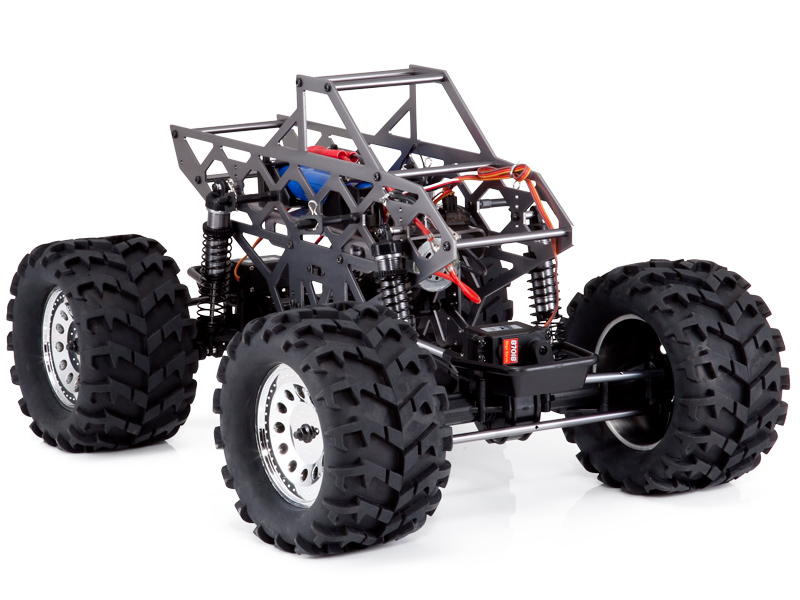
\includegraphics[width=10cm]{Chapters/Chapter2/Figures/groundpounder.jpg}
		\caption{Το τηλεκατευθυνόμενο όχημα \textit{GroundPounder}, της Redcat Racing.}
		\label{fig:groundpounder}
	\end{center}
\end{figure}

\bigskip
\subsection{Σασί Ρομποτικής Πλατφόρμας} \label{ssec:chassis}
Λόγω, της πληθώρας αισθητήρων, ηλεκτρονικού εξοπλισμού, καλωδιώσεων κλπ. και του περιορισμένου ελεύθερου χώρου πάνω στο όχημα, κρίθηκε σκόπιμο, αυτό, να επεκταθεί, με πρόσθετους χώρους. Για την λύση του προβλήματος, σχεδιάστηκαν, λοιπόν, και κατασκευάστηκαν, από μέλη της ομάδας P.A.N.D.O.R.A. 2014-15, δύο κουτιά, τα οποία προστέθηκαν επάνω στο υπάρχον όχημα, με σκοπό, να περιλάβουν τα επιμέρους υποσυστήματα του ρομπότ.

\begin{figure}[!ht]
	\centering
	\subfloat[Κουτί Τροφοδοσίας]{
		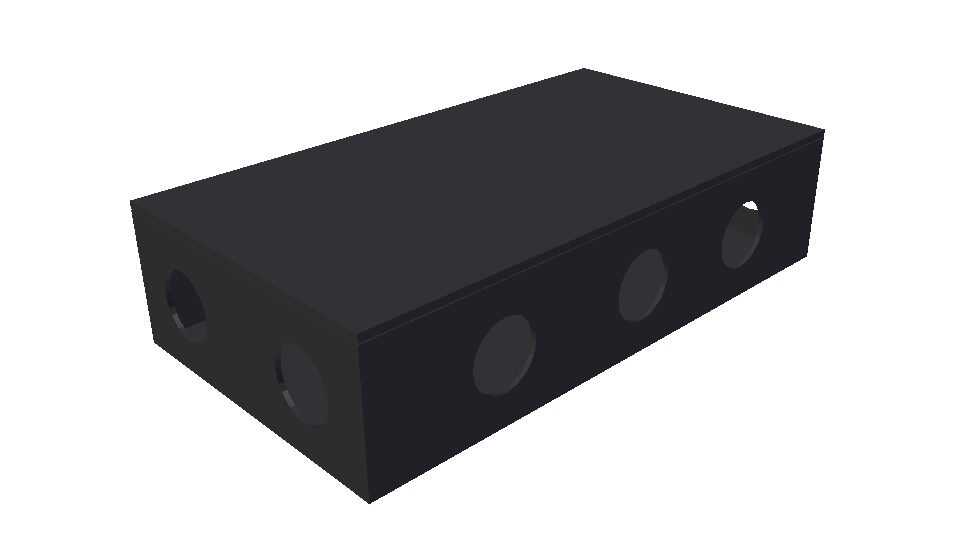
\includegraphics[width=0.45\linewidth]{Chapters/Chapter2/Figures/power_box.png}
		\label{fig:power_box}}
	\subfloat[Κουτί Ηλεκτρονικών]{
		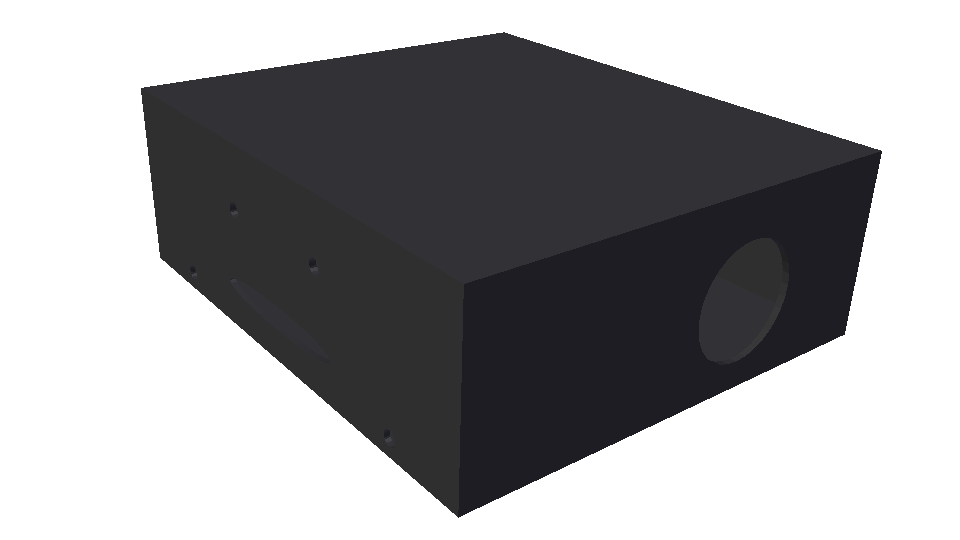
\includegraphics[width=0.45\linewidth]{Chapters/Chapter2/Figures/electronics_box.png}
		\label{fig:electronics_box}}
	\caption{Τα κουτιά του σασί της ρομποτικής πλατφόρμας Monstertruck.}
\end{figure}

\bigskip
Το \textit{κουτί τροφοδοσίας}, του σασί της ρομποτικής πλατφόρμας, που παρουσιάζεται στο σχήμα \ref{fig:power_box}, έχει διαστάσεις $310mm \times 170mm \times 74mm$, και περιλαμβάνει τρύπες, τοποθετημένες περιμετρικά του κουτιού, για πέρασμα καλωδιώσεων. Προορίζεται, όπως λέει και το όνομα του, για την τοποθέτηση του συστήματος τροφοδοσίας της ρομποτικής πλατφόρμας.

\bigskip
Το \textit{κουτί ηλεκτρονικών}, του σασί της ρομποτικής πλατφόρμας, που παρουσιάζεται στο σχήμα \ref{fig:electronics_box}, έχει διαστάσεις $210mm\times 240mm\times 84mm$, με δύο τρύπες στα πλάγια του ρομπότ, για τοποθέτηση ανεμιστήρων ψύξης του υπολογιστή, όπως, επίσης και ένα σύνολο από τρύπες στην μπροστινή πλευρά του κουτιού για κεραίες ασύρματης επικοινωνίας Wifi και καλωδιώσεις. Το \textit{κουτί ηλεκτρονικών}, προορίζεται για την τοποθέτηση του υπολογιστή, των αισθητήρων και των ελεγκτών της ρομποτικής πλατφόρμας.

\begin{figure}[!ht]
	\begin{center}
		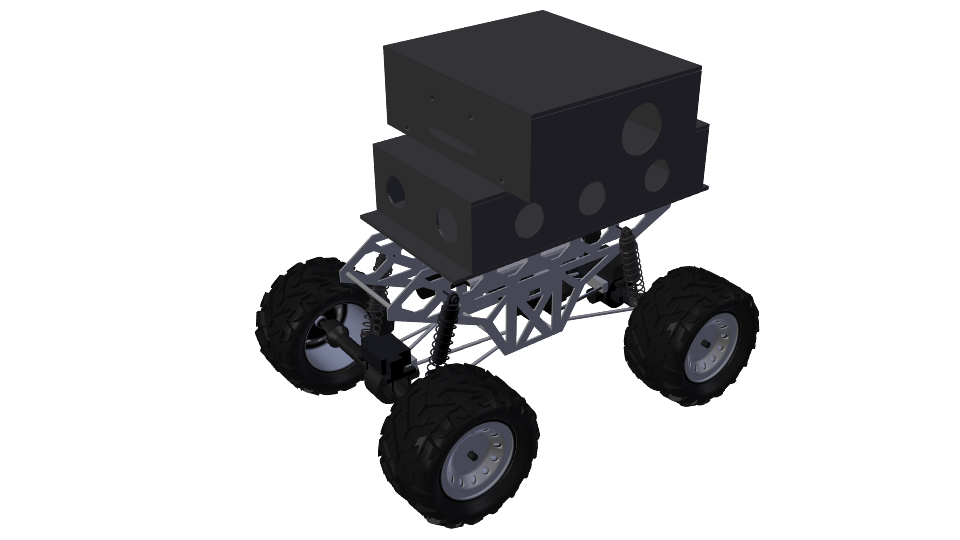
\includegraphics[width=10cm]{Chapters/Chapter2/Figures/base_diag.png}
		\caption{3D μοντέλο του συναρμολογημένου σασί της ρομποτικής πλατφόρμας Monstertruck.}
		\label{fig:chassis}
	\end{center}
\end{figure}

\bigskip
\subsection{Ηλεκτρονικός Εξοπλισμός} \label{ssec:electronic_equipment}
% σύστηματα τροφοδοσίας, υπολογιστής, αισθήτηρες, κινητήρες, σερβοκινητήρες και ελεγκτές

\bigskip
\subsubsection{Υπολογιστής} \label{sssec:computer}
Το πιο σημαντικό τμήμα ενός ρομποτικού συστήματος και ιδιαίτερα μίας αυτόνομης ρομποτικής πλατφόρμας αποτελεί ο εγκέφαλος του, δηλαδή, το υπολογιστικό του σύστημα, που του επιτρέπει να ελέγχει τα υποσυστήματα του και να εκτελεί διεργασίες και αλγορίθμους. Η επιλογή του υπολογιστικού συστήματος, που εν τέλει, εγκαταστάθηκε στην ρομποτική πλατφόρμα \textit{Monstertruck}, βασίστηκε σε δύο κριτήρια. Πρώτο και βασικότερο κριτήριο επιλογής αποτέλεσε η υπολογιστική ισχύς και κατά πόσο θα μπορούσε να εκτελεί τους απαιτούμενους αλγορίθμους ταυτόχρονα, αποδοτικά και χωρίς καθυστερήσεις. Το δεύτερο κριτήριο επιλογής, που λήφθηκε υπόψιν, ήταν, η κατανάλωση ισχύος, όσον αφορά τον χρόνο αυτονομίας.

\bigskip
Με βάση τα παραπάνω κριτήρια, τα υπολογιστικά συστήματα που εξετάστηκαν είναι το \textit{Raspberry Pi 2}, του \textit{Raspberry Pi Foundation} και το \textit{Odroid-XU4}, της \textit{Hardkernel}. Και οι δύο υπολογιστές, αυτοί, αποτελούν πλήρεις υπολογιστές, με Κεντρική Μονάδα Επεξεργασίας (CPU), μνήμη RAM, κάρτα γραφικών κλπ., σε εξαιρετικά μικρό μέγεθος και χαμηλή κατανάλωση ισχύος.

\begin{figure}[!ht]
	\begin{minipage}[t]{.49\textwidth}
 		\centering
		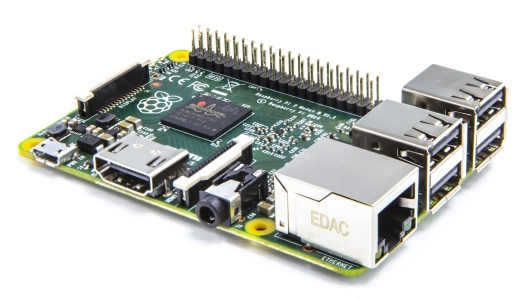
\includegraphics[width=0.6\linewidth]{Chapters/Chapter2/Figures/rpi2.jpg}
		\captionof{figure}{Raspberry Pi 2}
		\label{fig:rpi2}
	\end{minipage}
	\begin{minipage}[t]{.5\textwidth}		
		\centering
		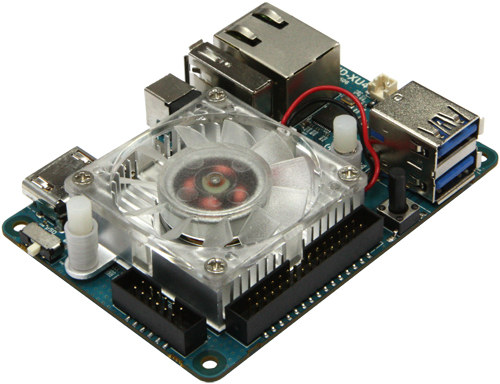
\includegraphics[width=0.5\linewidth]{Chapters/Chapter2/Figures/odroid-xu4.jpg}
		\captionof{figure}{Odroid-XU4}
		\label{fig:odroid-xu4}
	\end{minipage}
\end{figure}

\bigskip
\begin{table}[!ht]
	\centering
	\caption{Προδιαγραφές Raspberry Pi 2 και Odroid-XU4.}
	\begin{tabular}{| l | c | c |}
   		\hline
	   \textbf{Προδιαγραφές} & \textbf{Raspberry Pi 2} & \textbf{Odroid-XU4} \\ \hline
	   	CPU & Broadcom BCM2836 Arm7 & Samsung Exynos5422 ARM® \\ &Quad Core 900MHz Processor & Cortex™-A15 Quad 2.0GHz/\\ & & Cortex™-A7 Quad 1.4GHz\\ \hline
		GPU & Dual Core VideoCore IV® & Mali™-T628 MP6 OpenGL ES 3.0\\
		& Multimedia Co-Processor & / 2.0 / 1.1 and OpenCL 1.1 Full profile\\ 
		&  Open GL ES 2.0 &\\ \hline		   
	   Μνήμη RAM & 1GB LPDDR2 & 2GB LPDDR3 \\ \hline
	   Θύρες USB 2.0 & 4 & 1\\ \hline
	   Θύρες USB 3.0 & - & 2\\ \hline
	   Εικόνα & HDMI & HDMI\\ \hline
	   Ήχος & 4 pole Stereo output & HDMI Digital audio output\\ \hline
	   Αποθηκευτικός Χώρος & Micro SD & Micro SD ή eMMC 5.0\\ \hline
	   Ethernet & 10/100 & 10/100/1000\\ \hline
	  	Wifi & USB IEEE 802.11b/g/n & USB IEEE 802.11b/g/n 1T1R WLAN\\ \hline
	  	Περιφερειακά - & 40-pin GPIO, UART, SPI, I2C & UART, 30-pin GPIO/IRQ/SPI/ADC\\
	  	Διεπαφές & & 12-pin GPIO/I2S/I2C \\ \hline
	  	Τροφοδοσία & 5V, 2A & 5V, 4A\\ \hline
	   Διαστάσεις & $85 \times 56 \times 17 mm$ & $82 \times 58 \times 22 mm$\\\hline
   \end{tabular}
	\label{tab:computer_specs}
\end{table}

\newpage
Αρχικά, χρησιμοποιήθηκε, στην ρομποτική πλατφόρμα \textit{Monstertruck}, ο υπολογιστής \textit{Raspberry Pi 2}, αλλά, μετά από πειράματα και δοκιμές, με τους απαιτούμενους αλγορίθμους, για την αυτόνομη λειτουργία του οχήματος, διαπιστώθηκε, ότι, ο υπολογιστής \textit{Raspberry Pi 2}  είναι ανεπαρκής για την συγκεκριμένη εφαρμογή. Σαν αποτέλεσμα, στην ρομποτική πλατφόρμα, τελικά χρησιμοποιήθηκε ο υπολογιστής \textit{Odroid-XU4}, που μετά από αντίστοιχα πειράματα, η απόδοση του κρίθηκε πλήρως ικανοποιητική.

\bigskip
\subsubsection{Αισθητήρες} \label{sssec:sensors}
Μία εξαιρετικά σημαντική ιδιότητα, κάθε αυτόνομου ρομποτικού συστήματος, αποτελεί η αντίληψη του περιβάλλοντος του. Συγκεκριμένα, η ρομποτική αντίληψη στηρίζεται σε ένα σύνολο αισθητήρων, που επιτρέπουν στο ρομποτικό σύστημα να λαμβάνει πληροφορίες σχετικά με το περιβάλλον του, σε μορφή κατανοητή και αξιοποιήσιμη από αυτό.

\bigskip
Οι ρομποτικοί αισθητήρες, χωρίζονται σε κατηγορίες, ανάλογα με την πηγή της πληροφορίας, σε \textit{ιδιοδεκτικούς (proprioceptive)} ή \textit{εξωδεκτικούς (exteroceptive)} \cite{autonomous_mobile_robots}, εάν η πληροφορία προέρχεται από το ίδιο το ρομποτικό σύστημα, ή από το περιβάλλον του, αντίστοιχα. Παραδείγματα \textit{ιδιοδεκτικών} αισθητήρων, αποτελούν, οι \textit{αισθητήρες μέτρησης θέσης, ταχύτητας και ροπής των κινητήρων}, {γυροσκόπια}, {αισθητήρες μέτρησης της φόρτισης των μπαταριών} κα. Αντίστοιχα, \textit{εξωδεκτικοί} αισθητήρες, θεωρούνται, οι {αισθητήρες επαφής (tactile sensors)}, οι {ηλεκτρονικές πυξίδες (compass, IMU)}, αισθητήρες {GPS}, οι {υπέρυθροι, υπερηχητικοί και λέιζερ αισθητήρες απόστασης (range sensors)}, όπως επίσης και οι {κάμερες}. Επίσης, χωρίζονται και με βάση την πηγή εκπομπής της πληροφορίας \cite{autonomous_mobile_robots} σε \textit{παθητικούς (passive)}, εάν μετρούν κάποια μορφή ενέργειας που προέρχεται από το περιβάλλον και σε \textit{ενεργητικούς (active)}, εάν εκπέμπουν ενέργεια στο περιβάλλον και έπειτα, μετρούν την αντίδραση του περιβάλλοντος. Με βάση, τον συγκεκριμένο ορισμό, {αισθητήρες αφής}, {ηλεκτρονικές πυξίδες} και {κάμερες}, αποτελούν {παθητικούς} αισθητήρες, ενώ {κωδικοποιητές (encoders) κινητήρων}, {GPS}, {αισθητήρες απόστασης}, αποτελούν {ενεργητικούς} αισθητήρες. 

\bigskip
Ένα αυτόνομο ρομποτικό όχημα, είναι προφανές ότι απαιτεί αισθητήρες από όλες τις παραπάνω κατηγορίες για να μπορεί να αντιληφθεί και να κινηθεί μέσα στο περιβάλλον του, αλλά και να αντιδράσει μ' αυτό. Ακολούθως, παρουσιάζεται το σύνολο των αισθητήρων που περιλαμβάνει η ρομποτική πλατφόρμα \textit{Monstertruck}.

\bigskip
\begin{enumerate}
% Laser Scanner
\item \textit{Σαρωτής Λέιζερ (Laser Scanner)}:\\
Οι πιο σημαντικοί αισθητήρες για ένα αυτόνομο ρομποτικό όχημα είναι οι \textit{αισθητήρες απόστασης (range sensors)}, οι οποίοι του προσφέρουν πληροφορία, σχετικά με την απόσταση του οχήματος από εμπόδια, επιτρέποντας του, με αυτόν τον τρόπο, μέσω κατάλληλων αλγορίθμων, να χαρτογραφεί τον περιβάλλοντα χώρο του, να ξέρει ανά πάσα στιγμή τη θέση του και να πλοηγείται αυτόνομα μέσα σε αυτόν, αποφεύγοντας συγκρούσεις. 

Στην ρομποτική πλατφόρμα \textit{Monstertruck}, για τους παραπάνω λόγους, εγκαταστάθηκε ένας \textit{σαρωτής λέιζερ Hokuyo URG-04LX}. Η λειτουργία του βασίζεται στην τεχνική \textit{μέτρησης απόστασης, μέσω ανίχνευσης φωτός (Light Detection and Ranging ή LIDAR)}. Δηλαδή, εκπέμπει έναν παλμό ακτινοβολίας λέιζερ στο περιβάλλον προς μία κατεύθυνση και καταγράφοντας τον χρόνο που έκανε να επιστρέψει ο οπισθοσκεδαζόμενος παλμός, μπορεί να υπολογίσει την απόσταση του αισθητήρα από το περιβάλλον για εκείνη την κατεύθυνση. Πραγματοποιώντας την μέτρηση αυτή για ένα εύρος γωνιών, ο αισθητήρας προσφέρει μία δισδιάστατη αναπαράσταση του περιβάλλοντος που ουσιαστικά αποτελεί μία κάτοψη αυτού.

\begin{figure}[!ht]
	\begin{minipage}[t]{.49\textwidth}
 		\centering
		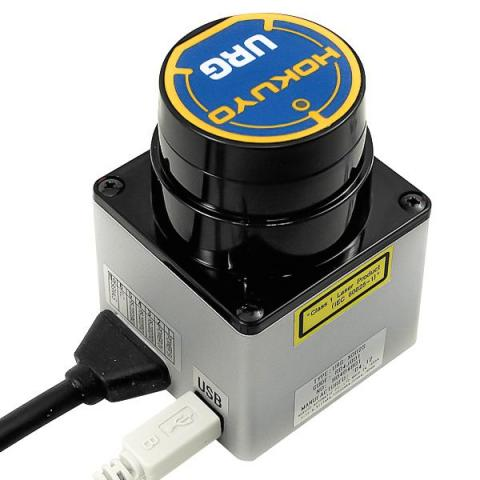
\includegraphics[width=0.6\linewidth]{Chapters/Chapter2/Figures/hokuyo.jpg}
		\captionof{figure}{Hokuyo URG-04LX.}
		\label{fig:hokuyo}
	\end{minipage}
	\begin{minipage}[t]{.49\textwidth}		
		\centering
 		\centering
		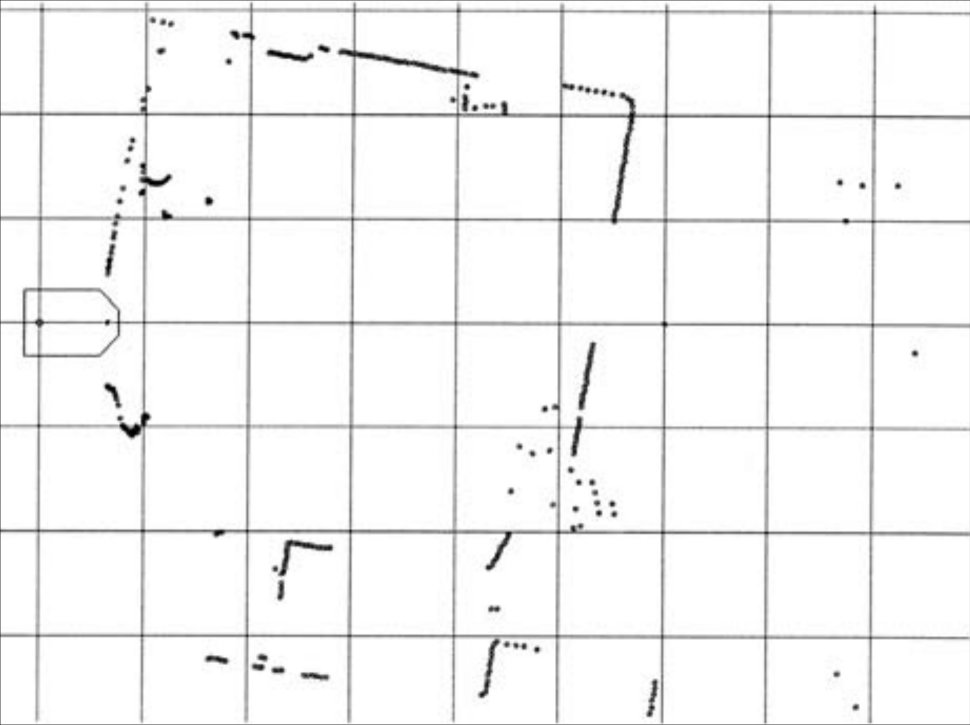
\includegraphics[width=0.75\linewidth]{Chapters/Chapter2/Figures/laser_scan.jpg}
		\captionof{figure}[Ενδεικτική σάρωση δωματίου.]{Ενδεικτική σάρωση δωματίου \cite{autonomous_land_vehicles}.}
		\label{fig:hokuyo_rays}
	\end{minipage}
\end{figure}

\bigskip

\begin{table}[!ht]
	\centering
	\captionof{table}{Προδιαγραφές Hokuyo URG-04LX}
	\label{tab:hokuyo_specs}
	\begin{tabular}{| l | c |}
		\hline
	   \textbf{Προδιαγραφές} & \textbf{Hokuyo URG-04LX} \\ \hline
	   Τροφοδοσία & 5VDC, 500mA\\ \hline
	   Εμβέλεια & 60 - 4\,095 mm \\ \hline
	   Περιοχή Μέτρησης & $240^{\circ}$\\ \hline
	   Ακρίβεια & $60 - 1000mm: \pm 10$ \\
   		& $1000 - 4095mm: 1\%$ \\ \hline
	  	Γωνιακή Ακρίβεια & $0.36^{\circ} (360^{\circ}/1024)$ \\ \hline
	  	Διεπαφή & USB, RS232 \\ \hline
	  	Διαστάσεις & $50 \times 50 \times 70 mm$ \\ \hline
	\end{tabular}
\end{table}

% IMU
\bigskip
\item \textit{Πυξίδα (Compass)}:\\
Ένα άλλο είδος αισθητήρων, ιδιαίτερα δημοφιλές και απαραίτητο στις περισσότερες ρομποτικές εφαρμογές αποτελούν οι \textit{αισθητήρες κατεύθυνσης (heading sensors)} \cite{autonomous_mobile_robots}. Στην κατηγορία, αυτή, ανήκουν τα {γυροσκόπια (gyroscopes)}, τα {κλινόμετρα (inclinometers)} και οι {πυξίδες (compasses)}. Οι αισθητήρες, αυτοί, χρησιμοποιούνται για να καθοριστούν ο {προσανατολισμός (orientation / yaw)} και η {κλίση (pitch, roll)} του ρομποτικού οχήματος, αλλά και σε συνδυασμό με μετρήσεις ταχύτητας για την εκτίμηση της θέσης του ({dead reckoning}).

Η ρομποτική πλατφόρμα {Monstertruck} χρησιμοποιεί την {πυξίδα Compass OS4000} της {Ocean Server}. Ο αισθητήρας αυτός, συνδυάζει ένα {μαγνητόμετρο (magnetometer)} τριών αξόνων και ένα {επιταχυνσιόμετρο (accelerometer)} τριών αξόνων. Το μαγνητόμετρο χρησιμοποιεί το μαγνητικό πεδίο της γης για να μετρήσει τον απόλυτο προσανατολισμό, ως προς τους τρεις άξονες $x, y, z$, ενώ το επιταχυνσιόμετρο μετράει μεταβολές στην ταχύτητα ως προς τους τρεις άξονες $x, y, z$.

\begin{figure}[!ht]
	\begin{minipage}[b]{0.45\textwidth}
		\centering
		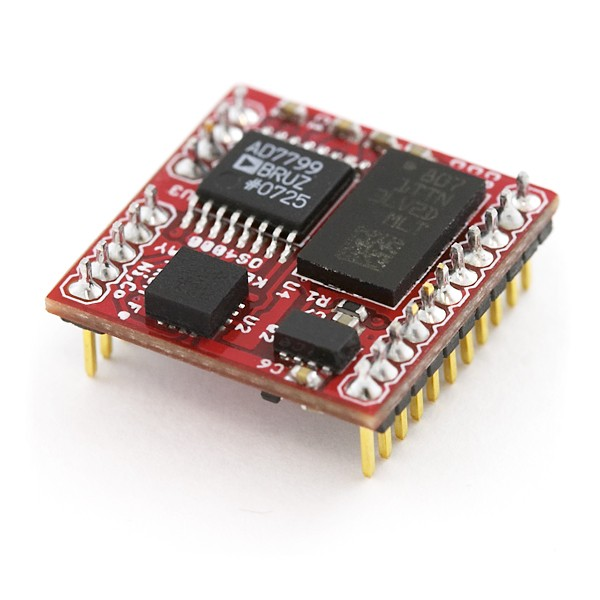
\includegraphics[width=0.5\linewidth]{Chapters/Chapter2/Figures/compassOS4000.jpg}
		\captionof{figure}{Compass OS4000.}
		\label{fig:compassOS4000}
	\end{minipage}		
	\begin{minipage}[b]{0.54\textwidth}
		\centering
		\captionof{table}{Προδιαγραφές Compass OS4000}
		\begin{tabular}{| l | c |}
			\hline
			\textbf{Προδιαγραφές} & \textbf{Compass OS4000}\\ \hline
			Τροφοδοσία & $3.3-5VDC, 30mA @ 3.3V$\\ \hline
			Σειριακή Διεπαφή& TTL 4800-115000 baud\\
			Επικοινωνίας  & 8 bit, 1 stop, no parity\\ \hline
			Συχνότητα & $0.01-40Hz$\\ \hline
			Ακρίβεια Αζιμούθιου & $<0.5^{\circ}, 0.1^{\circ}$ resolution\\ \hline
			Ακρίβεια Κλίσης & $<0.5^{\circ}, 0.1^{\circ}$ resolution\\ \hline
			Διαστάσεις & $15 \times 15 mm$\\ \hline
		\end{tabular}
		\label{tab:compassOS4000}
	\end{minipage}
\end{figure}

Η {πυξίδα Compass OS4000} χρησιμεύει για την, εύρεση της κλίσης (pitch, roll) του ρομπότ, έτσι ώστε να σταθεροποιείται στο οριζόντιο επίπεδο ο {σαρωτής λέιζερ}, που αναφέρθηκε παραπάνω, μέσω ενός μηχανισμού σταθεροποίησης pitch-roll, που αποτελείται από δύο σερβοκινητήρες. Παράλληλα, η πυξίδα χρησιμοποιείται και για στην εκτίμηση κατάστασης (θέση και προσανατολισμός) του οχήματος, συμπληρωματικά με άλλες πηγές εκτίμησης. Επίσης μπορεί να χρησιμοποιηθεί και για την επέκταση αλγορίθμων διάσχισης μονοπατιού, με βάση την ομαλότητα του εδάφους, βάση της τρέχουσα κλίσης του οχήματος, αλλά και σε ρουτίνες ασφαλείας, σε περίπτωση επικίνδυνων επιπέδων κλίσης του οχήματος, που μπορεί να προκαλέσουν ανατροπή.

% Camera
\bigskip
\item \textit{Κάμερα}:\\
Η όραση αποτελεί την πιο ισχυρή αίσθηση του ανθρώπου. Προσφέρει έναν τεράστιο όγκο πληροφορίας για το περιβάλλον και διευκολύνει την αλληλεπίδραση του με αυτό. Στα ρομποτικά συστήματα, η αίσθηση της όρασης προσεγγίζεται με {κάμερες}, οι οποίες καταγράφουν την ίδια πληροφορία, σε μεγάλο βαθμό, που συγκεντρώνει και το ανθρώπινο μάτι.

Στα ρομποτικά συστήματα, {κάμερες}, μπορεί να χρησιμοποιούνται για επίβλεψη και χειρισμό ρομποτικών συστημάτων, αλλά μεγαλύτερο ενδιαφέρον παρουσιάζει ο κλάδος της {ρομποτικής όρασης} που ασχολείται με την δημιουργία αλγορίθμων που εξάγουν πληροφορία από τις εικόνες που παράγει μία {κάμερα}. Για παράδειγμα, {κάμερες} και αλγόριθμοι {ρομποτικής όρασης} χρησιμοποιούνται για αναγνώριση αντικειμένων, προσώπων και προτύπων, γενικότερα, αλλά ακόμα και σε χαρτογράφηση περιβάλλοντος και εκτίμηση κατάστασης   (Visual SLAM) κα.

Στην ρομποτική πλατφόρμα {Monstertruck}, είναι εγκατεστημένη μία απλή web κάμερα Logitech Portable Webcam C905, η οποία χρησιμοποιήθηκε στα πλαίσια της παρούσας εργασίας, μονάχα για επίβλεψη κατά τον χειρισμό ή την αυτόνομη λειτουργία της ρομποτικής πλατφόρμας. Παρόλα αυτά, όπως αναφέρθηκε παραπάνω, με την εκμετάλλευση της πληροφορίας από την κάμερα, μέσω κατάλληλων αλγορίθμων, η λειτουργικότητα της ρομποτικής πλατφόρμας μπορεί να επεκταθεί σημαντικά.

\begin{figure}[!ht]
	\centering
	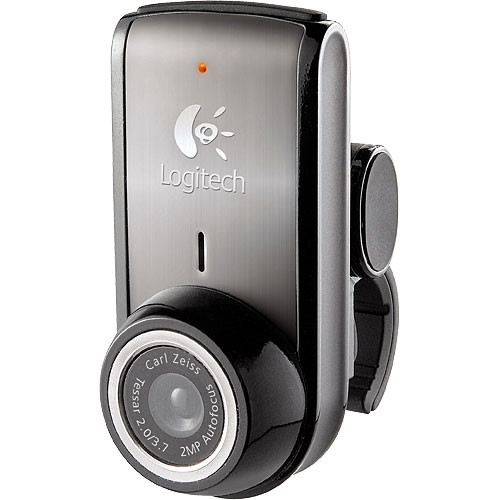
\includegraphics[width=.3\linewidth]{Chapters/Chapter2/Figures/webcam.jpg}
	\caption{Logitech Portable Webcam C905.}
	\label{fig:webcam}
\end{figure}


% motor encoders, hall sensors
\bigskip
\item \textit{Αισθητήρες Θέσης και Ταχύτητας Κινητήρων}:\\
Σε κινούμενα ρομποτικά συστήματα, όπως είναι προφανές, χρησιμοποιούνται κινητήρες και σερβοκινητήρες. Για τον ακριβή έλεγχο και παρακολούθηση αυτών, είναι απαραίτητη η ύπαρξη αισθητήρων που προσφέρουν πληροφορία σχετικά με την θέση, ταχύτητα, επιτάχυνση, φορτίο, ρεύμα, τροφοδοσία ή θερμοκρασία, κατά την λειτουργία τους. Στη ρομποτική πλατφόρμα {Monstertruck}, χρησιμοποιείται ένας {αισθητήρες Hall} για τον κινητήρα των τροχών και {κωδικοποιητές (encoders)} για τον κινητήρα και τους σερβοκινητήρες του οχήματος.

Ο \textit{αισθητήρας Hall} είναι ένας μετατροπέας που μεταβάλλει την τάση εξόδου του, ως αντίδραση στις μεταβολές ενός μαγνητικού πεδίου. Στους κινητήρες χρησιμοποιείται ως μετρητής των στροφών ανά λεπτό. Είναι οικονομικός αισθητήρας, μπορεί να δουλέψει σε υψηλές συχνότητες και δεν επηρεάζεται από φαινόμενα θορύβου μηχανικών επαφών (contact bounce), αλλά, έχει μικρή ακρίβεια και είναι επιρρεπείς σε σφάλματα ολίσθησης (drift).

Οι \textit{κωδικοποιητές} είναι μία κατηγορία αισθητήρων που χρησιμοποιούνται για την μέτρηση της θέσης ή ταχύτητας του άξονα ενός κινητήρα. Η μέτρηση αυτή χρησιμοποιείται από το κύκλωμα κλειστού βρόχου ενός κινητήρα για έλεγχο θέσης ή ταχύτητας. Οι απλοί {συμβατικοί σερβοκινητήρες (hobby servos)} του εμπορίου χρησιμοποιούν {περιστροφικούς κωδικοποιητές} σε μορφή ποτενσιομέτρων ({rotary / shaft encoders}) που μεταβάλλουν την τάση εξόδου τους, ανάλογα με την θέση του άξονα του σερβοκινητήρα. Αντίθετα, οι {βιομηχανικοί κινητήρες}, συνήθως χρησιμοποιούν {οπτικούς κωδικοποιητές (optical encoders)}, οι οποίοι, αποτελούνται από έναν δίσκο με διαφανείς και αδιαφανείς περιοχές και ζεύγη φωτοεκπομπών και φωτοδεκτών, που διαβάζουν τα μοτίβα του δίσκου και συμπεραίνουν την θέση του άξονα του κινητήρα.

\begin{figure}[!ht]
	\centering
	\subfloat[Αισθητήρας Hall Κινητήρα.]{
		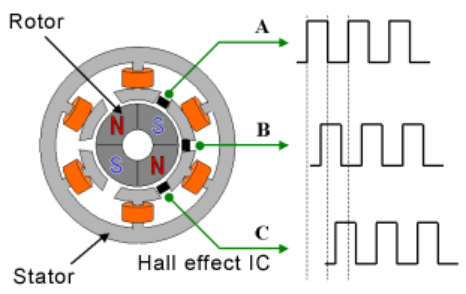
\includegraphics[width=0.3\linewidth]{Chapters/Chapter2/Figures/motor_hall_effect.png}
		\label{fig:hall_sensor}}
	\subfloat[Σερβοκινητήρας με περιστροφικό κωδικοποιητή.]{
		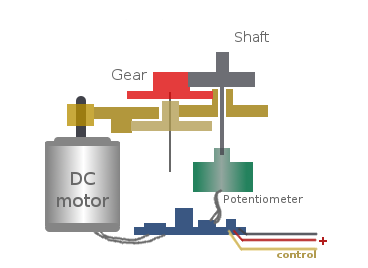
\includegraphics[width=0.35\linewidth]{Chapters/Chapter2/Figures/servo_internals.png}
		\label{fig:rotary_encoder}}\\
	\subfloat[Οπτικός κωδικοποιητής.]{
		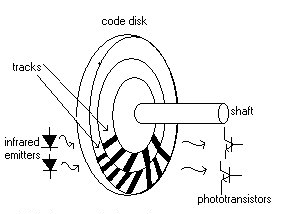
\includegraphics[width=0.3\linewidth]{Chapters/Chapter2/Figures/optical_encoder.png}
		\label{fig:optical_encoder}}
	\caption{Αισθητήρες θέσης και ταχύτητας κινητήρων.}
\end{figure}


% battery monitor
\bigskip
\item \textit{Αισθητήρας Μέτρησης Τάσης Μπαταρίας}:\\
Η ρομποτική πλατφόρμα \textit{Monstertruck} τροφοδοτείται μέσω επαναφορτιζόμενων μπαταριών \textit{Λιθίου - Πολυμερών (LiPo)} που συνδυάζουν υψηλή χωρητικότητα, μικρό όγκο και βάρος, σε σύγκριση με άλλους τύπους μπαταριών. Ένα σημαντικό πρόβλημα των μπαταριών \textit{LiPo} είναι η ασφάλεια τους, καθώς σε περίπτωση υπερφόρτισης, αποφόρτισης, βραχυκυκλώματος, κρούσης ή διείσδυσης μπορεί να προκληθεί καταστροφική ζημιά, όπως ρήξη συσκευασίας, διαρροή ηλεκτρολύτη και φωτιά. Επίσης, κακή χρήση της μπαταρίας, μέσω υπερφορτίσεων και αποφορτίσεων πέρα από τα επιτρεπτά επίπεδα, προκαλεί μείωση της χωρητικότητας και του χρόνου ζωής της μπαταρίας. Καθίσταται, επομένως, απαραίτητη η χρήση ενός αισθητήρα που θα μετρά τα επίπεδα τάσης της μπαταρίας και θα τα μεταδίδει στον κεντρικό υπολογιστή του ρομποτικού συστήματος, στον οποίο θα λειτουργεί μία διεργασία που θα λαμβάνει την πληροφορία αυτή, θα την επεξεργάζεται κατάλληλα (πχ. φιλτράρισμα θορύβου) και θα εξάγει συμπεράσματα και θα ειδοποιεί τον επιβλέπον / χειριστή, σε περίπτωση που η μπαταρία χρειάζεται φόρτιση ή σε περίπτωση που παρεκκλίνει από τα επιτρεπτά όρια.

Για την μέτρηση της τάσης της μπαταρίας, απαιτείται ένας αισθητήρας που θα μετατρέπει την αναλογική τάση σε ψηφιακή πληροφορία. Τον σκοπό αυτό εξυπηρετούν οι \textit{Μετατροπείς Αναλογικού Σήματος σε Ψηφιακό (ADC)}, οι οποίοι μετατρέπουν μία αναλογική τάση σε έναν ψηφιακό αριθμό. Η διαδικασία της μετατροπής, περιλαμβάνει κβαντισμό και περιοδική δειγματοληψία της τάσης εισόδου και σαν αποτέλεσμα εισάγει ένα μικρό σφάλμα μετατροπής, το οποίο στην προκειμένη περίπτωση, δεν επηρεάζει σημαντικά την εφαρμογή. Οι αισθητήρες \textit{ADC} περιγράφονται, συνήθως, από μία μέγιστη τάση εισόδου (πχ. $5V$). Επειδή, όμως στην ρομποτική πλατφόρμα χρησιμοποιούνται μπαταρίες LiPo με ονομαστική τάση $22.2V$ (μέγιστη τάση $25.2V$), απαιτείται μία κλιμάκωση της τάσης εισόδου. Για τον λόγο αυτό, η τάση εισόδου του μετατροπέα ADC κλιμακώνεται μέσω ενός διαιρέτη τάσης με σχέση 1:10 από 0-25.2V σε 0-2.52V. Επίσης, λόγω των μεγάλων διαταραχών στην τάση της μπαταρίας, κατά την λειτουργία της ρομποτικής πλατφόρμας, χρησιμοποιήθηκε ένα \textit{χαμηλοπερατό φίλτρο RC}.

\begin{figure}[!ht]
	\centering
	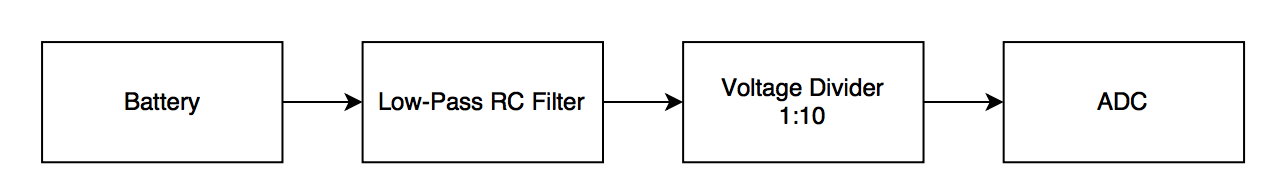
\includegraphics[width=0.8\linewidth]{Chapters/Chapter2/Figures/rc_filter_divider.png}
	\caption{Στάδια επεξεργασίας τάσης μπαταρίας για μέτρηση της σε ADC.}
	\label{fig:rc_filter_divider}
\end{figure}

\end{enumerate}
%%%%%%%%%%%%%%%%%%%%%%%%%%%%%%%%%%%%%%%%%%%%%%%%%%%%%%%%%%%%%%%%%%%%%%%%%%%%%%%%%%%%%%%%%%%%%%

\subsubsection{Κινητήρας} \label{sssec:motor}
Το τηλεκατευθυνόμενο όχημα GroundPounder, αρχικά, περιλάμβανε έναν {Brushed DC ηλεκτρικό κινητήρα}, με μέγιστη ταχύτητα, περίπου, $30\,000rpm$, ο οποίος ελεγχόταν από έναν ελεγκτή {ESC} (Electronic Speed Controller), με δυνατότητες ελέγχου ταχύτητας και φοράς. Παρόλα αυτά, λόγω της μικρής ακρίβειας ελέγχου ταχύτητας και την απουσία {κωδικοποιητή} ή άλλων αισθητήρων για την παροχή μετρήσεων, σχετικά με την πραγματική ταχύτητα του κινητήρα κάθε στιγμή, σε συνδυασμό, με τις υψηλές απαιτήσεις ακριβείας των ρομποτικών εφαρμογών, κρίθηκε σκόπιμο, το εν λόγω σύστημα κινητήρα και ελεγκτή να αντικατασταθεί.

\begin{figure}[!ht]
	\begin{minipage}{.49\textwidth}
 	\centering
		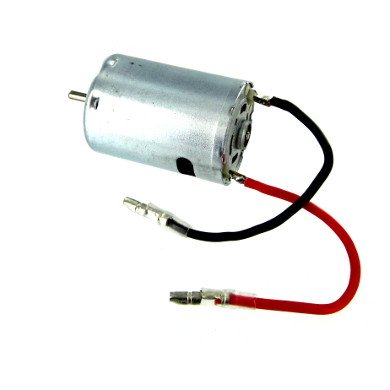
\includegraphics[width=0.6\linewidth]{Chapters/Chapter2/Figures/original_motor.jpg}
		\captionof{figure}{
			Ο κινητήρας Brushed 540 του τηλεκατευθυνόμενου οχήματος GroundPounder.}
		\label{fig:original_motor}
	\end{minipage}
	\begin{minipage}{.5\textwidth}		
		\centering
		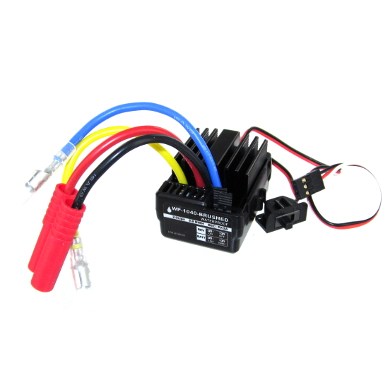
\includegraphics[width=0.6\linewidth]{Chapters/Chapter2/Figures/esc.jpg}
		\captionof{figure}{
			Ο ελεγκτής ESC B7003SR του τηλεκατευθυνόμενου οχήματος GroundPounder.}
		\label{fig:esc}
	\end{minipage}
\end{figure}

Για την αντικατάσταση, λοιπόν, του παραπάνω συστήματος κινητήρα και ελεγκτή, επιλέχθηκαν από τον διαθέσιμο εξοπλισμό της ομάδας {P.A.N.D.O.R.A}, ένας κινητήρας με αντίστοιχο ελεγκτή, της εταιρείας {maxon motor}. Ο κινητήρας \textit{maxon EC-max 283858}, είναι ένας {Brushless EC κινητήρας} με μέγιστη ταχύτητα $18000rpm$, με {ψηφιακό κωδικοποιητή (encoder)} για μέτρηση της θέσης του άξονα του κινητήρα, όπως επίσης και {αισθητήρα Hall} για μέτρηση των στροφών του κινητήρα ανά λεπτό. Επίσης, περιλαμβάνει ένα gearbox με λόγο μετάδοσης 1:66. 

\bigskip
Αντίστοιχα, ως ελεγκτής, επιλέχθηκε ο {EPOS 24/1}, της {maxon motor}. Ο ελεγκτής αυτός, αποτελεί ένα μικρού μεγέθους ψηφιακό έξυπνο ελεγκτή, με δυνατότητες ελέγχου 
θέσης, ταχύτητας και ρεύματος, αλλά και δυνατότητες μέτρησης θέσης και ταχύτητας του κινητήρα.

\begin{figure}[!ht]
	\begin{minipage}[b]{.49\textwidth}		
		\centering
		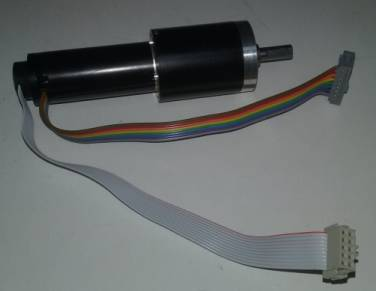
\includegraphics[width=0.8\linewidth]{Chapters/Chapter2/Figures/maxon_motor_ec_283858.jpg}
		\captionof{figure}{
			Ο κινητήρας maxon EC-max 283858, με κωδικοποιητή και μειωτήρα στροφών.}
		\label{fig:maxon_motor}
	\end{minipage}
	\begin{minipage}[b]{.5\textwidth}
 	\centering
		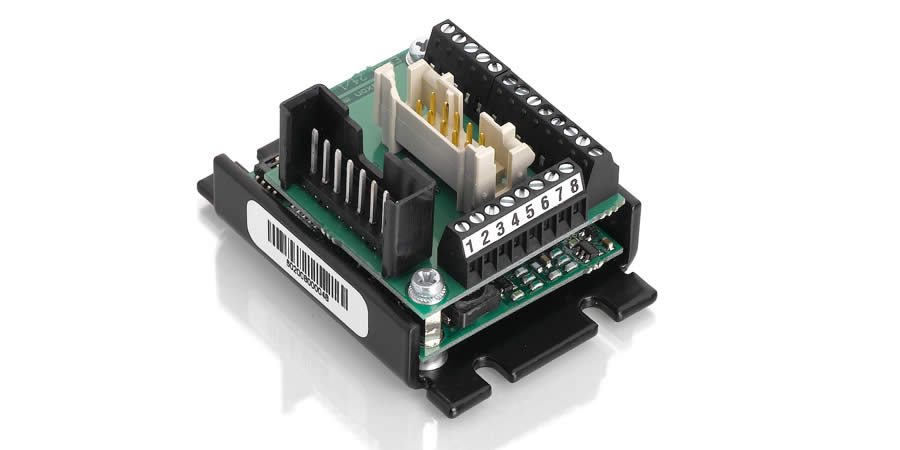
\includegraphics[width=0.8\linewidth]{Chapters/Chapter2/Figures/epos241.jpg}
		\captionof{figure}[Ο έξυπνος ελεγκτής κινητήρα, EPOS 24/1, της maxon motor.]{
			Ο έξυπνος ελεγκτής κινητήρα, EPOS 24/1, της maxon motor \cite{epos241_manual}.}	
		\label{fig:epos241}
	\end{minipage}
\end{figure}

Ο κινητήρας συνδέεται με τον ελεγκτή {EPOS 24/1} μέσω δύο καλωδίων, ένα για τον έλεγχο του κινητήρα και για λήψη μετρήσεων από τον {αισθητήρα Hall} και το άλλο, για λήψη μετρήσεων από τον {ψηφιακό κωδικοποιητή}. Ο ελεγκτής {EPOS 24/1}, επίσης, απαιτεί σύνδεση σε τροφοδοσία 9-24VDC, 1Α, ενώ παράλληλα, για επικοινωνία με ηλεκτρονικό υπολογιστή, χρησιμοποιεί το πρωτόκολλο επικοινωνίας {RS232} χωρίς χειραψία, μέσω της ελάχιστης συνδεσμολογίας {RS232} (RX, TX, Ground).

\begin{figure}[!ht]
		\centering
		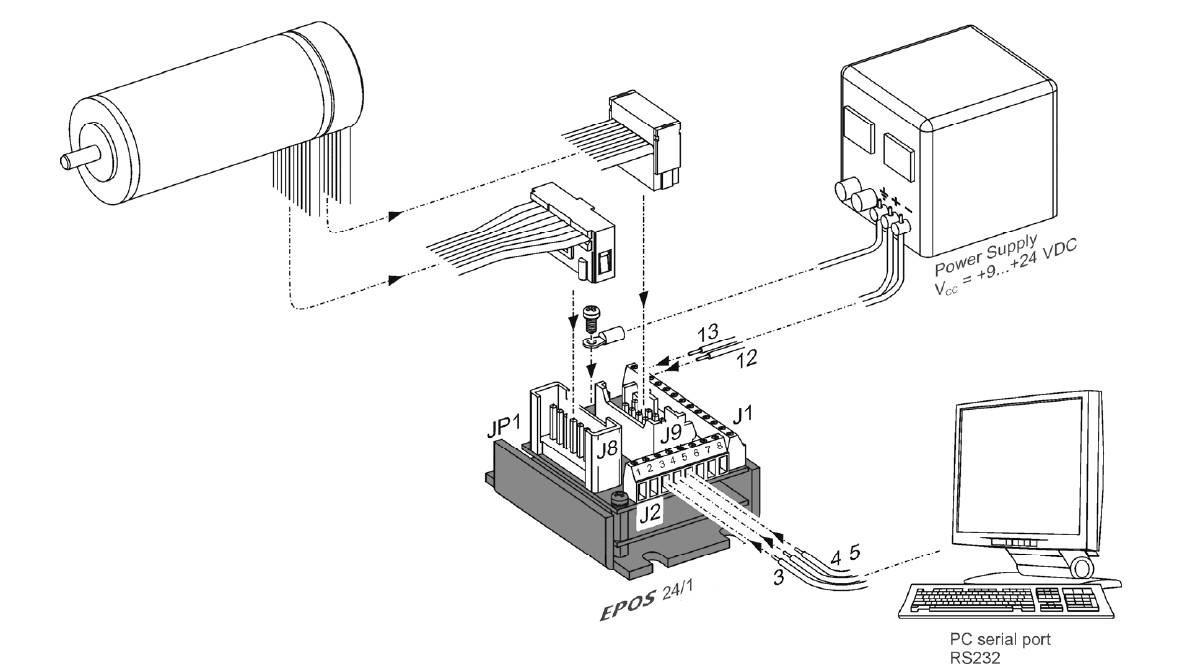
\includegraphics[width=0.6\linewidth]{Chapters/Chapter2/Figures/motor_minimum_wiring.jpg}
		\caption[Καλωδίωση Κινητήρα, Ελεγκτή και Υπολογιστή.]{Καλωδίωση Κινητήρα, Ελεγκτή και Υπολογιστή \cite{epos241_manual}.}
		\label{fig:motor_minimum_wiring}
\end{figure}

O ελεγκτής {EPOS 24/1}, όπως προαναφέρθηκε, επιτρέπει την επικοινωνία με τον κεντρικό υπολογιστή της ρομποτικής πλατφόρμας, μέσω του πρωτοκόλλου διεπαφής {RS232}. Παρόλα αυτά, ο κεντρικός υπολογιστής δεν διαθέτει διεπαφή {RS232} και επομένως, απαιτείται ένας ενδιάμεσος κόμβος, ο οποίος θα καθιστά δυνατή την επικοινωνία μεταξύ τους. Το ρόλο αυτό, στην προκειμένη περίπτωση, εξυπηρετεί ένα {μετατροπέας διεπαφής RS232 σε USB} (σχήμα \ref{fig:rs232_to_usb_adapter}).

\begin{figure}[!ht]
		\centering
		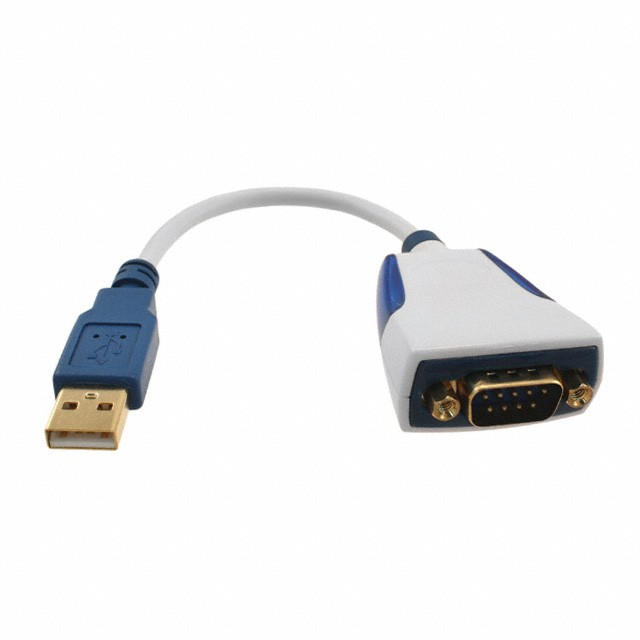
\includegraphics[width=.3\linewidth]{Chapters/Chapter2/Figures/rs232_to_usb_adapter.jpg}
		\caption{Μετατροπέας διεπαφής RS232 σε USB.}
		\label{fig:rs232_to_usb_adapter}
\end{figure}

\bigskip
\subsubsection{Σερβοκινητήρες} \label{sssec:servos}
Οι σερβοκινητήρες είναι συστήματα κινητήρων που επιτρέπουν ακριβή έλεγχο θέσης, ταχύτητας και επιτάχυνσης. Οι {συμβατικοί σερβοκινητήρες} αποτελούνται από έναν DC κινητήρα, σε συνδυασμό με {γρανάζια μετάδοσης}, έναν {αισθητήρα θέσης}, συνήθως {περιστροφικό κωδικοποιητή (rotary encoder)} και ένα κύκλωμα ελέγχου. Οι απλοί συμβατικοί σερβοκινητήρες ελέγχονται μέσω σημάτων Διαμόρφωσης Πλάτους Παλμού (PWM), αλλά υπάρχει, βέβαια, και μία κατηγορία σερβοκινητήρων, οι λεγόμενοι {έξυπνοι σερβοκινητήρες (smart servo motors)}, οι οποίοι έχουν ενσωματωμένο μικροελεγκτή. Ο μικροελεγτκής αυτός, προσφέρει, υψηλότερη ακρίβεια ελέγχου, ευρωστία στο θόρυβο και αμφίδρομη επικοινωνία, μέσω σειριακού πρωτοκόλλου, συνήθως {TTL Full-Duplex} ή {Half-Duplex} και {RS485}. Τέλος, ένα σημαντικό πλεονέκτημα των έξυπνων σερβοκινητήρων, έναντι των συμβατικών, είναι η παροχή μετρήσεων θέσης (position feedback), ικανότητα εξαιρετικής σημασίας για ρομποτικές εφαρμογές.

\bigskip
Στην ρομποτική πλατφόρμα {Monstertruck} χρησιμοποιούνται συνολικά τέσσερις σερβοκινητήρες, δύο από τους οποίους είναι {συμβατικοί} και οι άλλοι δύο {έξυπνοι}.

\bigskip
Οι δύο {συμβατικοί σερβοκινητήρες} χρησιμοποιούνται στο σύστημα {τετραδιεύθυνσης} της ρομποτικής πλατφόρμας που θα αναλυθεί στην αντίστοιχη ενότητα, είναι τύπου {Hitek HS-M7990TH}, με ροπή $44 kg \cdot cm $ στα $6V$ και ανάλυση $0.082°/\mu sec$.

\bigskip
Ο έλεγχος των δύο σερβοκινητήρων πραγματοποιείται από έναν ελεγκτή {Micro Maestro 6 - Channel USB Servo Controller} της {Pololu}. Ο ελεγκτής, αυτός, προσφέρει αποδοτικό έλεγχο σερβοκινητήρων, υψηλής ακρίβειας, με ενσωματωμένο έλεγχο ταχύτητας και επιτάχυνσης, έξι κανάλια ελέγχου και επικοινωνία μέσω σειριακού πρωτοκόλλου {USB}.

\begin{figure}[!ht]
	\begin{minipage}[t]{.49\textwidth}		
		\centering
		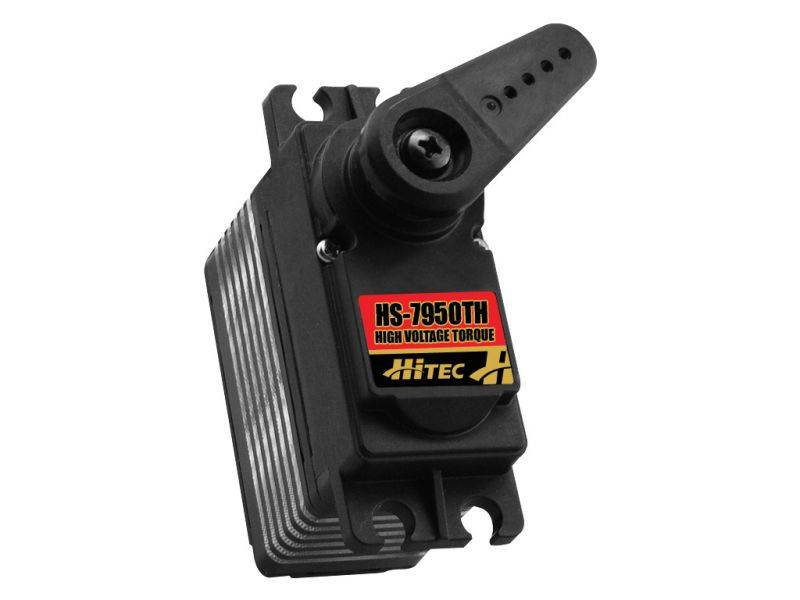
\includegraphics[width=0.5\linewidth]{Chapters/Chapter2/Figures/hitek_servo.jpg}
		\caption{Σερβοκινητήρας Hitek HS-7954TH.}
		\label{fig:hitek_servo}
	\end{minipage}
	\begin{minipage}[t]{.5\textwidth}
 	\centering
		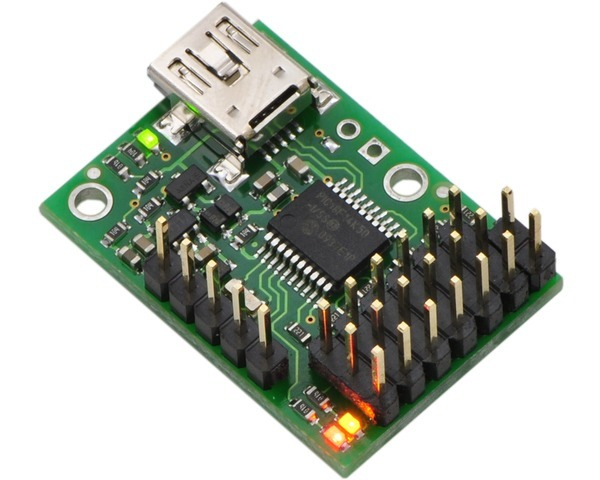
\includegraphics[width=0.5\linewidth]{Chapters/Chapter2/Figures/pololu_maestro.jpg}
		\captionof{figure}{Pololu Micro Maestro 6-Channel USB Servo Controller}
		\label{fig:pololu_maestro}
	\end{minipage}
\end{figure}

\begin{figure}[!ht]
		\centering
		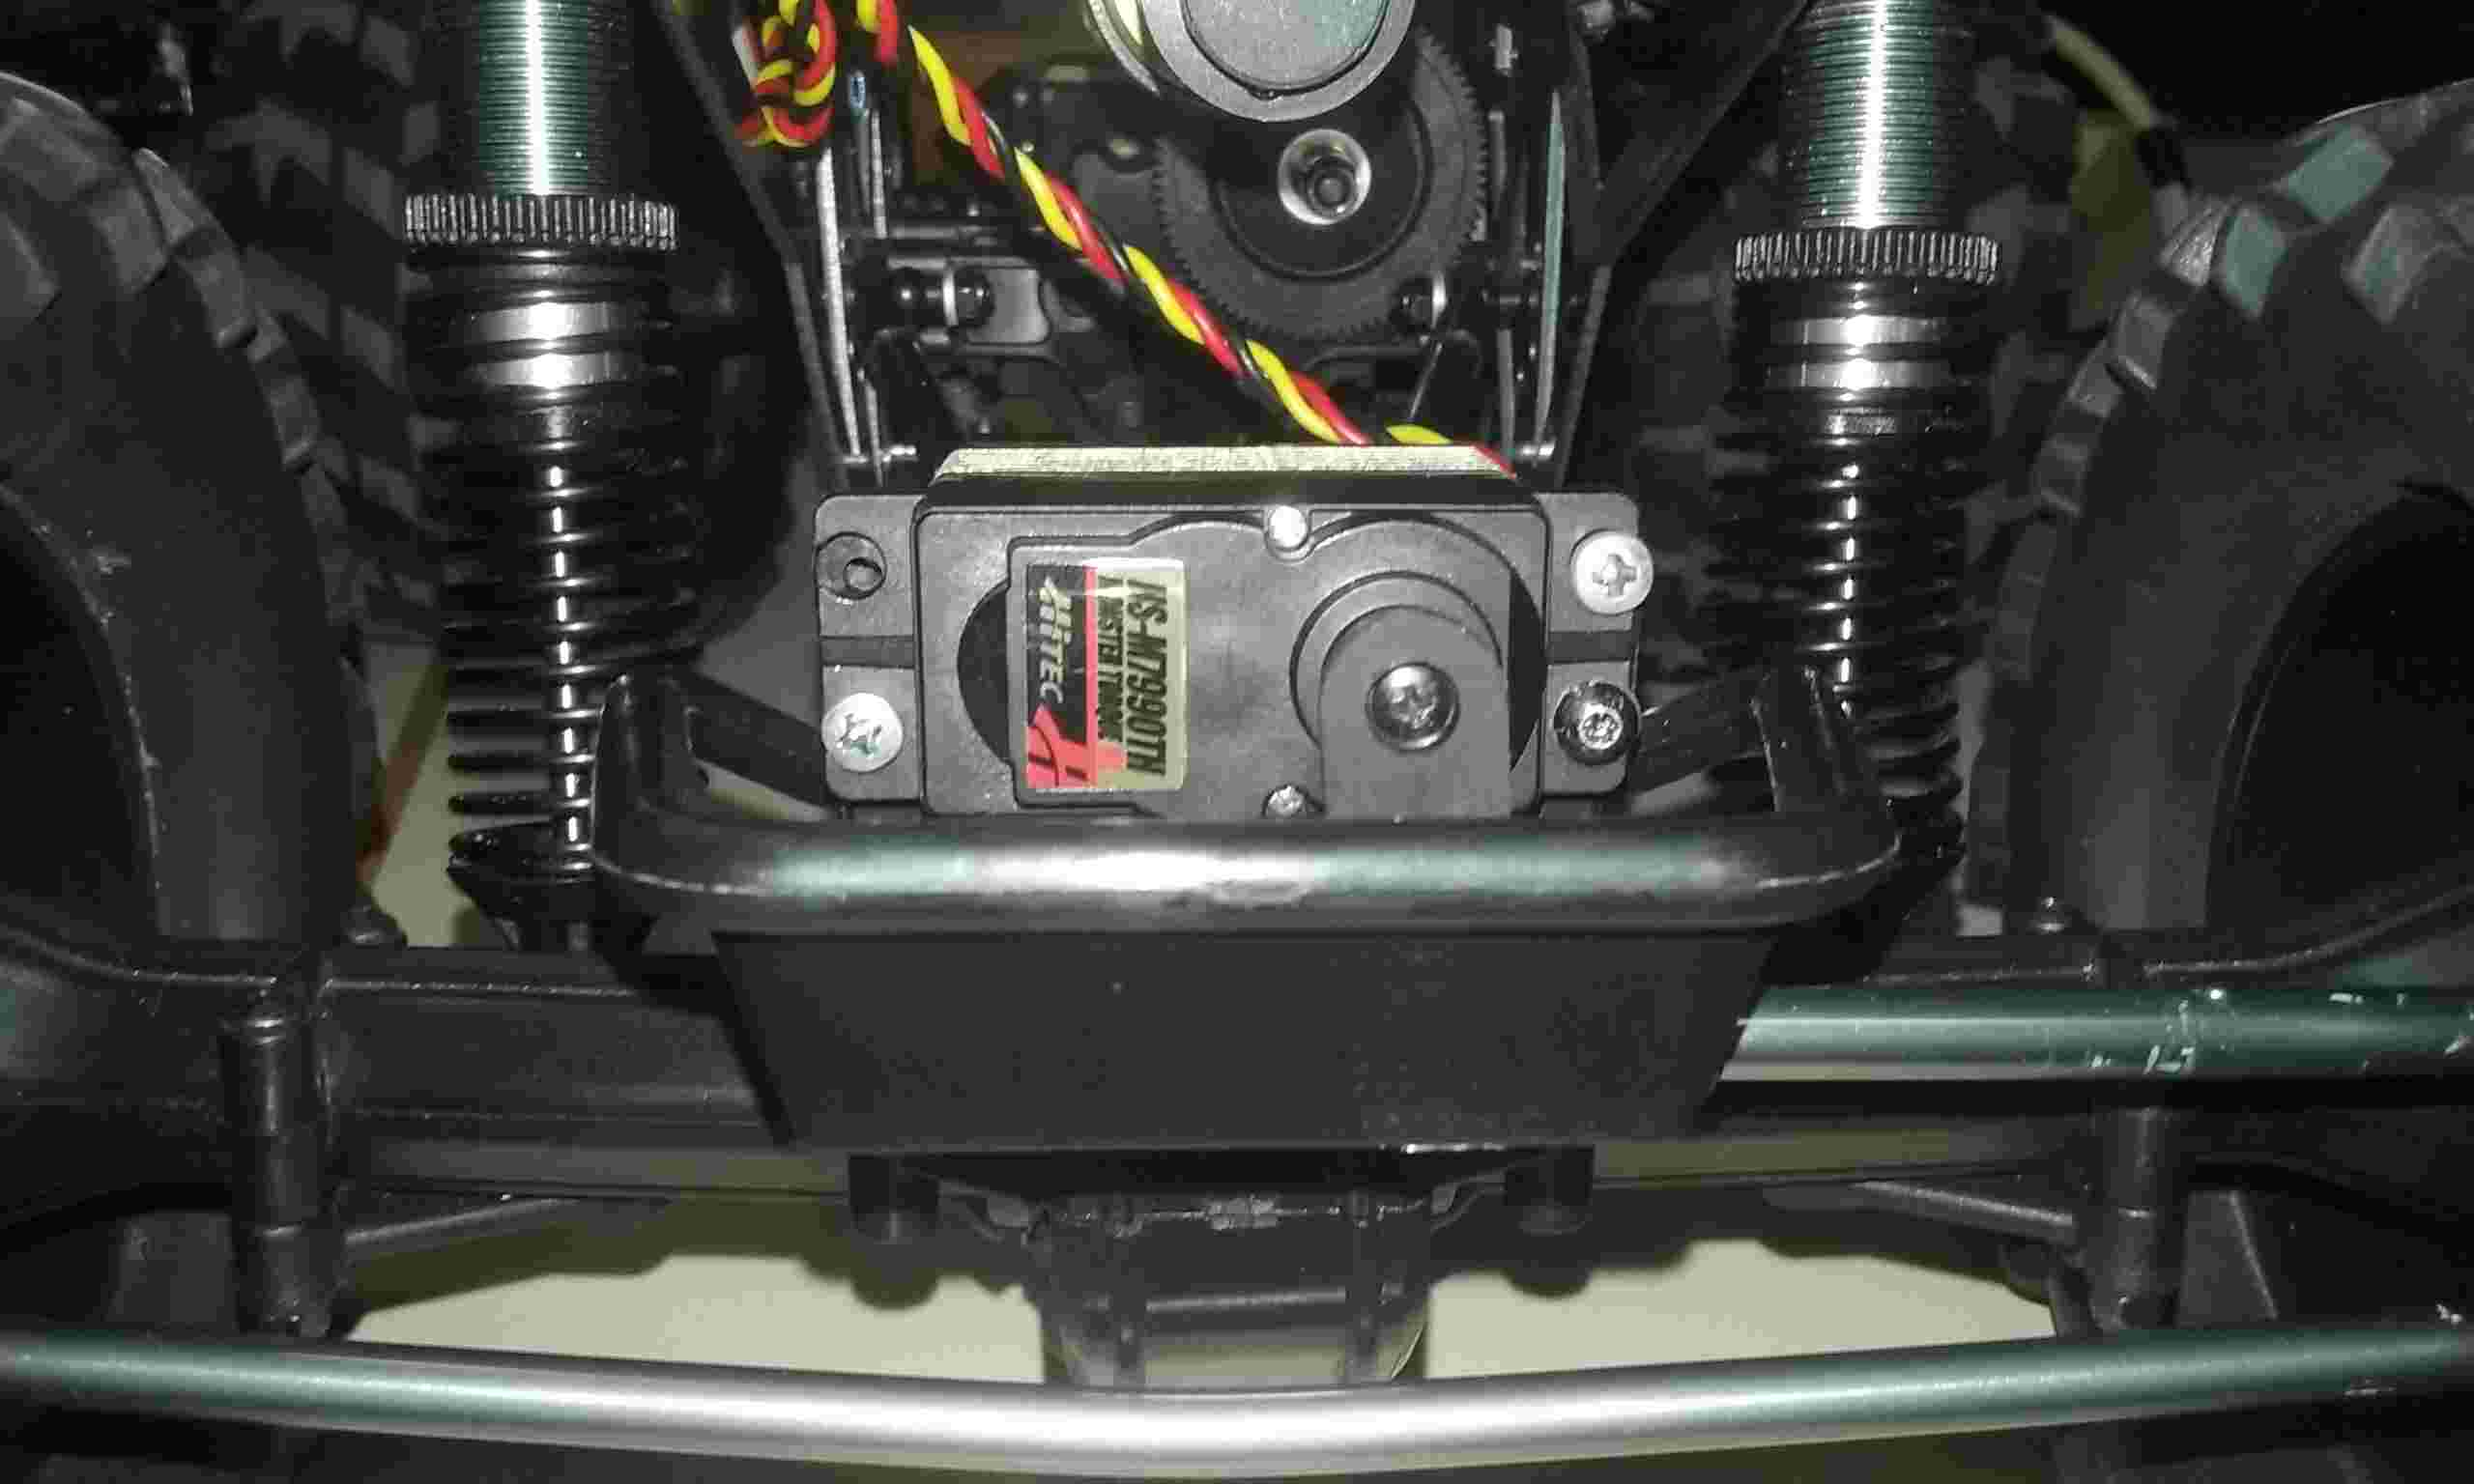
\includegraphics[width=0.5\linewidth]{Chapters/Chapter2/Figures/steering_servo.jpg}
		\caption{O Σερβοκινητήρας Hitek HS-7954TH πάνω στην ρομποτική πλατφόρμα Monstertruck.}
		\label{fig:servo_steering}
\end{figure}

\bigskip
Οι δύο {έξυπνοι σερβοκινητήρες}, χρησιμοποιούνται ως {μηχανισμός σταθεροποίησης (Pitch-Roll Stabilizer)} του {Σαρωτή Λέιζερ}, που αναφέρθηκε παραπάνω, λαμβάνοντας υπόψιν πληροφορία για την κλίση του οχήματος μέσω της πυξίδας {Compass OS4000}. Ο μηχανισμός αυτός είναι απαραίτητος για την αξιόπιστη χαρτογράφηση χώρου με ανώμαλο έδαφος.

\bigskip
Οι {έξυπνοι σερβοκινητήρες} του {μηχανισμού σταθεροποίησης} του {Σαρωτή Λέιζερ}, είναι τύπου {Dynamixel AX-12A}, της {Robotis}. Οι {έξυπνοι σερβοκινητήρες Dynamixel AX-12} έχουν την δυνατότητα να παίρνουν μετρήσεις, σχετικά με την ταχύτητα, θέση, θερμοκρασία, τάση και φορτίο και να αντιδρούν ανάλογα με την περίπτωση και να μεταδίδουν αυτήν την πληροφορία στον υπολογιστή του ρομποτικού συστήματος.

\begin{figure}[!ht]
	\begin{minipage}[b]{0.45\textwidth}
		\centering
		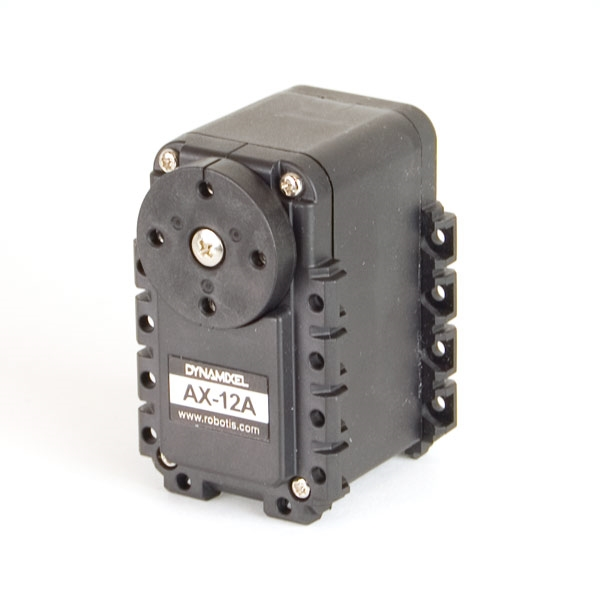
\includegraphics[width=0.8\linewidth]{Chapters/Chapter2/Figures/dxl_ax_12a.jpg}
		\caption{Σερβοκινητήρας Dynamixel\\ AX-12A, της Robotis.}
		\label{fig:dxl_ax_12a}
	\end{minipage}		
	\begin{minipage}[b]{0.475\textwidth}
		\centering
		\captionof{table}{Προδιαγραφές σερβοκινητήρα\\ Dynamixel AX-12A, της Robotis}
		\begin{tabular}{| l | c |}
			\hline
			\textbf{Προδιαγραφές} & \textbf{Dynamixel AX-12A}\\ \hline
			Τροφοδοσία & $9-12VDC, 900mA$\\ \hline
			Σειριακή Διεπαφή& 3-pin TTL Half-Duplex\\
			Επικοινωνίας  & 7343bps ~ 1Mbps\\ \hline
			Εύρος & $300^{\circ}$\\ \hline
			Μέγιστη Ροπή & $15.3 kg \cdot cm$\\ \hline
			Μέγιστη Ταχύτητα & 59 RPM \\ (χωρίς φορτίο) & 0.169sec/60°\\ \hline
			Feedback & Θέσης, Φορτίου,\\& Θερμοκρασίας, Τάσης\\ \hline
			Διαστάσεις & $32 \times 50 \times 40 mm$\\ \hline
		\end{tabular}
		\label{tab:dxl_ax_12a_specs}
	\end{minipage}
\end{figure}


\bigskip
Η επικοινωνία, μεταξύ του υπολογιστή και των {έξυπνων σερβοκινητήρων}, επιτυγχάνεται μέσω του {αντάπτορα USB2Dynamixel}, ο οποίος επικοινωνεί με τον υπολογιστή μέσω σειριακού πρωτοκόλλου {USB} και με τους {έξυπνους σερβοκινητήρες} μέσω σειριακής επικοινωνίας {TTL}. Επίσης, οι δύο {έξυπνοι σερβοκινητήρες} συνδέονται μεταξύ τους σειριακά, μέσω τοπολογίας {Daisy Chain}.

\begin{figure}[!ht]
	\begin{minipage}[t]{.49\textwidth}
 	\centering
		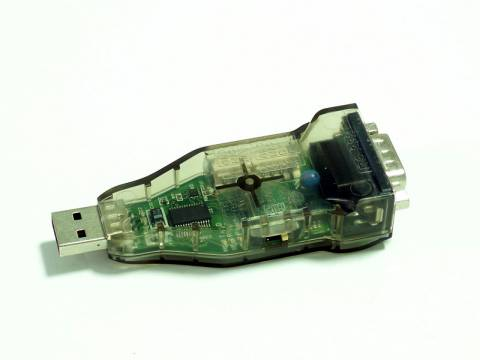
\includegraphics[width=0.6\linewidth]{Chapters/Chapter2/Figures/usb2dynamixel.jpg}
		\captionof{figure}{Αντάπτορας USB2Dynamixel,\\ της Robotis.}
		\label{fig:usb2dynamixel}
	\end{minipage}
	\begin{minipage}[t]{.5\textwidth}		
		\centering
		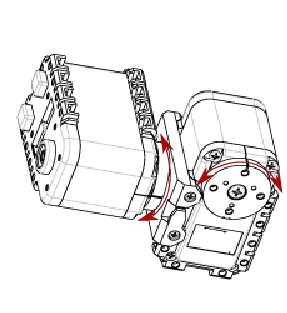
\includegraphics[width=0.5\linewidth]{Chapters/Chapter2/Figures/pitch_roll_dxl.png}
		\caption{Διάταξη Pitch-Roll του\\ σταθεροποιητή του σαρωτή λέιζερ.}
		\label{fig:pitch_roll_dxl}
	\end{minipage}
\end{figure}

\bigskip
\subsubsection{Ασύρματη Επικοινωνία} \label{sssec:wireless_communication}
Η προετοιμασία και ο χειρισμός της ρομποτικής πλατφόρμας {Monstertruck} ή η επίβλεψη της, κατά την αυτόνομη λειτουργία από τον χειριστή/επιβλέποντα, απαιτεί έναν πρόσθετο υπολογιστή, ο οποίος θα συνιστά τον {σταθμό χειρισμού/επίβλεψης}. Η επικοινωνία μεταξύ των δύο υπολογιστικών συστημάτων, μπορεί να πραγματοποιηθεί, είτε ενσύρματα, μέσω μίας διασύνδεσης διεπαφής {Ethernet}, είτε ασύρματα, μέσω ενός πομποδέκτη ασύρματης επικοινωνίας {Wi-Fi}, σε συνδυασμό με έναν {δρομολογητή Wi-Fi (Wi-Fi router)} που αποτελεί και την πιο πρακτική λύση, αν αναλογιστεί κανείς, ότι σε αντίθετη περίπτωση, ο χειριστής θα έπρεπε να κυνηγάει το ρομπότ από πίσω, με κίνδυνο πρόκλησης ατυχήματος, πιθανή αποσύνδεση, αλλά και πιθανή παρεμβολή στις μετρήσεις των αισθητήρων. H απαίτηση αυτή, ικανοποιείται στη ρομποτική πλατφόρμα {Monstertruck}, μέσω ενός αντάπτορα {TP-Link WiFi N900 TL-WDN4200}.

\bigskip
\begin{figure}[!ht]
	\begin{minipage}[b]{0.4\textwidth}
		\centering
		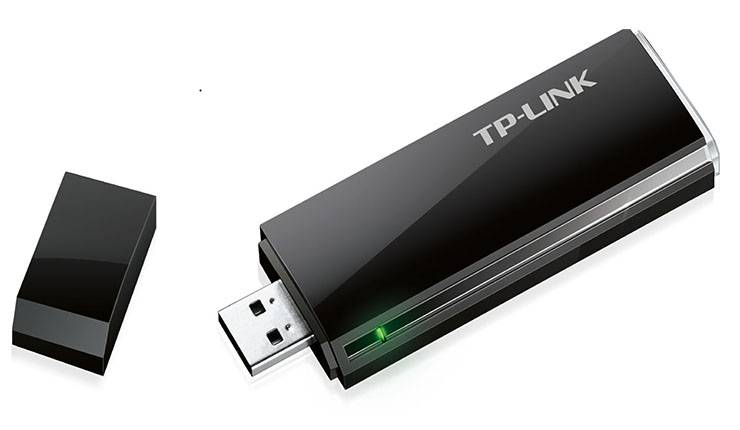
\includegraphics[width=0.6\linewidth]{Chapters/Chapter2/Figures/wifi_adapter.jpg}
		\caption{TP-Link Wi-Fi USB\\ Adapter N900 TL-WDN4200.}
		\label{fig:wifi_adapter}
	\end{minipage}		
	\begin{minipage}[b]{0.5\textwidth}
		\centering
		\captionof{table}{Προδιαγραφές TP-Link Wi-Fi USB\\ Adapter N900 TL-WDN4200.}
		\begin{tabular}{| l | c |}
			\hline
			\textbf{Προδιαγραφές} & \textbf{TP-Link Wi-Fi USB Adapter}\\
			 &  \textbf{N900 TL-WDN4200}\\ \hline
			Σύνδεση & USB 2.0 \\ \hline
			Ταχύτητα & Dual Band $2 \times 450Mbps$\\ \hline
			Πρότυπο & IEEE 802.11b/g/n\\ \hline
			Συχνότητα & 2.4/5GHz\\ \hline
			Ασφάλεια & WEP (64-128bit)\\ \hline
		\end{tabular}
		\label{tab:wifi_adapter_specs}
	\end{minipage}
\end{figure}


\bigskip
\subsubsection{Διασύνδεση Υποσυστημάτων} \label{sssec:interconnections}
Στις παραπάνω ενότητες αναφέρθηκαν τα επιμέρους υποσυστήματα της ρομποτικής πλατφόρμας {Monstertruck} και έγινε φανερό, ότι δεν χρησιμοποιούνται οι ίδιες διεπαφές επικοινωνίας σε κάθε συσκευή, αλλά και ότι κάθε συσκευή, χρησιμοποιεί το δικό της πρωτόκολλο επικοινωνίας. Το μόνο κοινό όλων των υποσυστημάτων, είναι η διασύνδεση και η συγκέντρωση της πληροφορίας, στον κεντρικό κόμβο του συστήματος, τον υπολογιστή {Odroid-XU4}.

\bigskip
Ένα σημαντικό πρόβλημα, του υπολογιστή {Odroid-XU4}, αποτελεί ο ανεπαρκής, για την συγκεκριμένη εφαρμογή, αριθμός θυρών διεπαφής σειριακής επικοινωνίας USB. Επομένως, για την ταυτόχρονη λειτουργία όλων των επιμέρους αισθητήρων και ελεγκτών του συστήματος, κρίθηκε απαραίτητη η προσθήκη δύο {διακλαδωτών USB (USB Hubs)}(σχήμα \ref{fig:usb_hubs}X). Η διασύνδεση των διεπαφών, όλων των επιμέρους υποσυστημάτων της ρομποτικής πλατφόρμας \textit{Monstertruck}, παρουσιάζεται στο σχήμα \ref{fig:hardware_interface_diagram}.

\begin{figure}[!ht]
	\centering
	\subfloat[Akasa AK-HB-01-BK 4-port USB hub Black.]{
		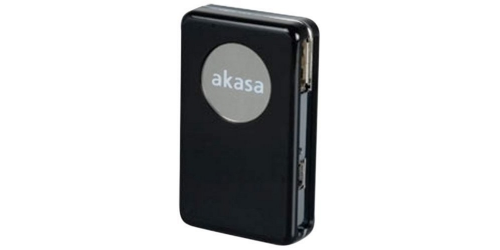
\includegraphics[width=0.33\linewidth]{Chapters/Chapter2/Figures/usb_hub_black.png}
		\label{fig:usb_hub_black}}
	\subfloat[Akasa AK-HB-01WH C 4-PORT USB hub White.]{
		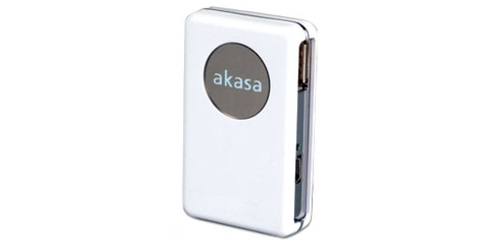
\includegraphics[width=0.33\linewidth]{Chapters/Chapter2/Figures/usb_hub_white.png}
		\label{fig:usb_hub_white}}
	\caption{Οι διακλαδωτές σειριακής διεπαφής USB (USB Hubs) της ρομποτικής  πλατφόρμας Monstertruck.}
	\label{fig:usb_hubs}
\end{figure}


\begin{figure}[!ht]
	\centering
	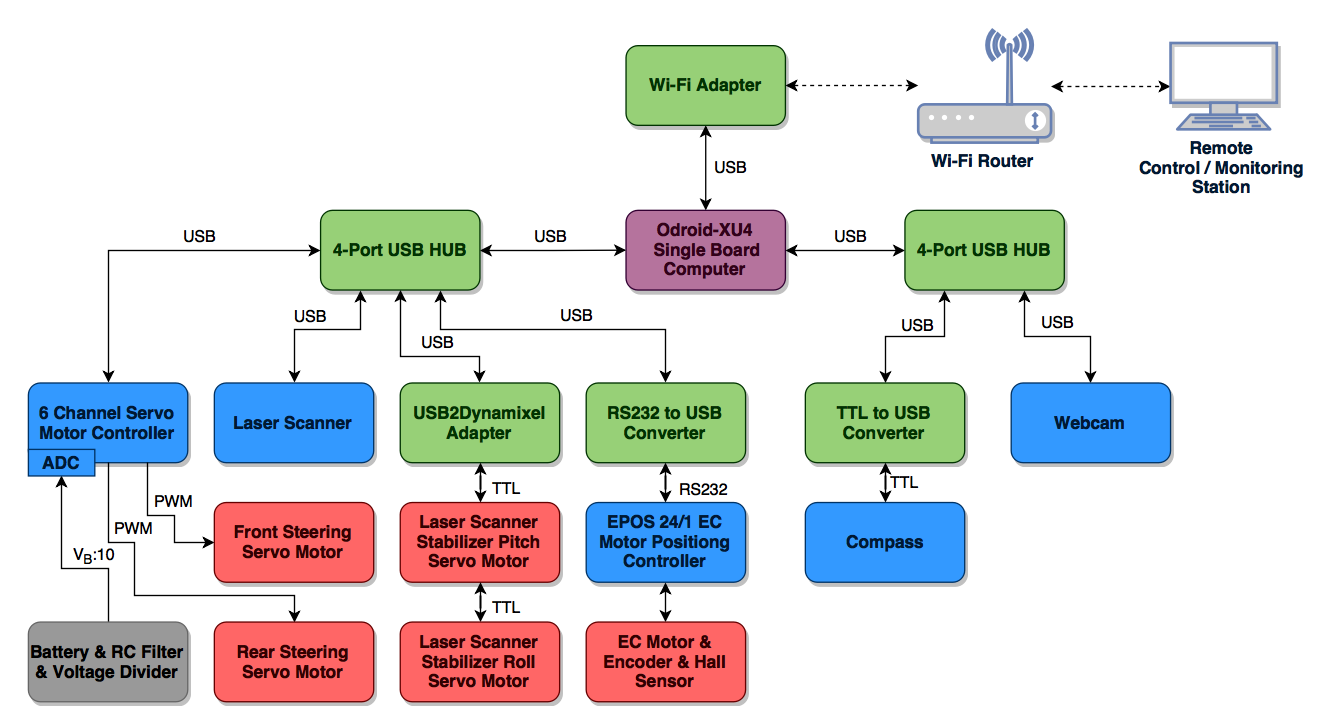
\includegraphics[width=1\linewidth]{Chapters/Chapter2/Figures/hardware_interface_diagram.png}
	\caption{Διασύνδεση διεπαφών των επιμέρους υποσυστημάτων της ρομποτικής πλατφόρμας \textit{Monstertruck}.}
	\label{fig:hardware_interface_diagram}
\end{figure}


\bigskip
\subsubsection{Σύστημα Τροφοδοσίας} \label{sssec:power_supply}
Από την παρουσίαση των επιμέρους υποσυστημάτων της ρομποτικής πλατφόρμας {Monstertruck}, που πραγματοποιήθηκε στις προηγούμενες παραγράφους, προκύπτει, ότι, κάθε υποσύστημα - συσκευή, περιλαμβάνει διαφορετικές προδιαγραφές τροφοδοσίας. Επομένως, απαιτείται, ένα εκτενές και πλήρες σύστημα τροφοδοσίας που να προσφέρει τις απαιτούμενες προδιαγραφές για κάθε υποσύστημα ξεχωριστά, για την ταυτόχρονη λειτουργία, όλων μαζί, αλλά και να επιτρέπει περιθώρια επέκτασης. Επίσης, θα πρέπει να περιλαμβάνει επαρκής απομόνωση της τροφοδοσίας των ευαίσθητων ηλεκτρονικών υποσυστημάτων, από άλλα υποσυστήματα που εισάγουν θόρυβο στις γραμμές τροφοδοσίας, όπως οι κινητήρες και οι σερβοκινητήρες. 

\bigskip
Όπως παρουσιάζεται και στο σχήμα \ref{fig:power_distribution}, ως πηγή τροφοδοσίας της ρομποτικής πλατφόρμας {Monstertruck}, χρησιμοποιείται μία μπαταρία {Λιθίου-Πολυμερών} (σχήμα \ref{fig:battery}) με ονομαστική τάση 22.2V, μέγιστη τάση 25.2V ($100\%$ φόρτιση) και 3700/4000/5000mAh. Η τροφοδοσία που παρέχει η μπαταρία, τροφοδοτείται σε έναν {διακλαδωτή (Battery Distribution Board)}, από τον οποίο τροφοδοτούνται ο ελεγκτής {EPOS 24/1} που τροφοδοτεί και τον κινητήρα του οχήματος, ο {12V DC-DC μετατροπέας} και το {τροφοδοτικό M4-ATX}.

\begin{figure}[!ht]
	\centering
	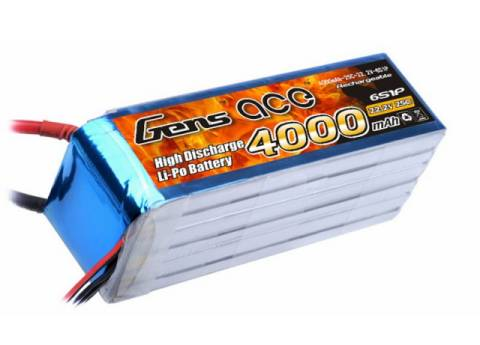
\includegraphics[width=0.25\linewidth]{Chapters/Chapter2/Figures/battery.jpg}
	\caption{Μπαταρία Gens ace, LiPo, 22.2V, 4000mAh.}
	\label{fig:battery}
\end{figure}

\bigskip
Ο {12V DC-DC μετατροπέας} τροφοδοτεί με 12V, μέσω ενός {διακλαδωτή (Motor Distribution Board)} τους {έξυπνους σερβοκινητήρες Dynamixel} του {σταθεροποιητή Pitch-Roll} του {σαρωτή λέιζερ}, όπως επίσης και έναν ανεμιστήρα, υπεύθυνο για την ψύξη του υπολογιστή {Odroid-XU4}.

\bigskip
Το τροφοδοτικό {M4-ATX} παράγει εξόδους τροφοδοσίας 5V και 12V και τροφοδοτεί την πλειονότητα των ηλεκτρονικών υποσυστημάτων της ρομποτικής πλατφόρμας. Αρχικά, τροφοδοτεί απευθείας έναν {5V DC-DC μετατροπέα}, ο οποίος χρησιμοποιείται για να τροφοδοτεί τους σερβοκινητήρες του συστήματος στρέψης των τροχών της ρομποτικής πλατφόρμας, απομονώνοντας, ταυτόχρονα την τροφοδοσία των σερβοκινητήρων από την τροφοδοσία των υπόλοιπων ηλεκτρονικών υποσυστημάτων που παρουσιάζουν ευαισθησία στον θόρυβο. Τα υπόλοιπα ηλεκτρονικά υποσυστήματα της ρομποτικής πλατφόρμας, τροφοδοτούνται από το τροφοδοτικό {M4-ATX}, μέσω ενός {διακλαδωτή (Electronics Distribution Board)}, είτε άμεσα, όπως ο υπολογιστής {Odroid-XU4}, ο {σαρωτής λέιζερ} και οι {διακλαδωτές USB (USB Hubs)}, είτε μέσω του υπολογιστή και των {διακλαδωτών USB}.

\begin{figure}[!ht]
	\centering
	\subfloat[Τροφοτικό M4-ATX.]{
		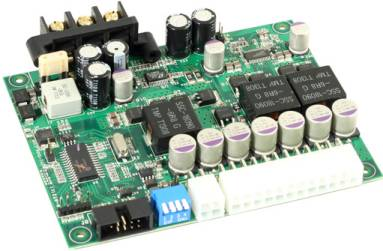
\includegraphics[width=0.3\linewidth]{Chapters/Chapter2/Figures/m4atx.jpg}
		\label{fig:m4atx}}
	\subfloat[5V DC-DC Μετατροπέας.]{
		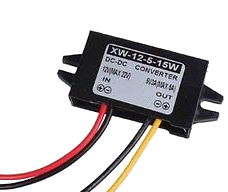
\includegraphics[width=0.3\linewidth]{Chapters/Chapter2/Figures/5v_dc_dc_converter.png}
		\label{fig:5v_dc_dc_converter}}
	\subfloat[12V DC-DC Μετατροπέας.]{
		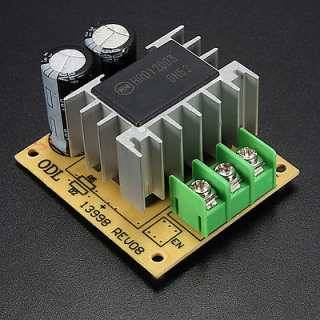
\includegraphics[width=0.3\linewidth]{Chapters/Chapter2/Figures/12v_dc_dc_converter.jpg}
		\label{fig:12v_dc_dc_converter}}
	\caption{Επιμέρους τμήματα συστήματος τροφοδοσίας.}
\end{figure}

\bigskip
\begin{figure}[!ht]
	\centering
	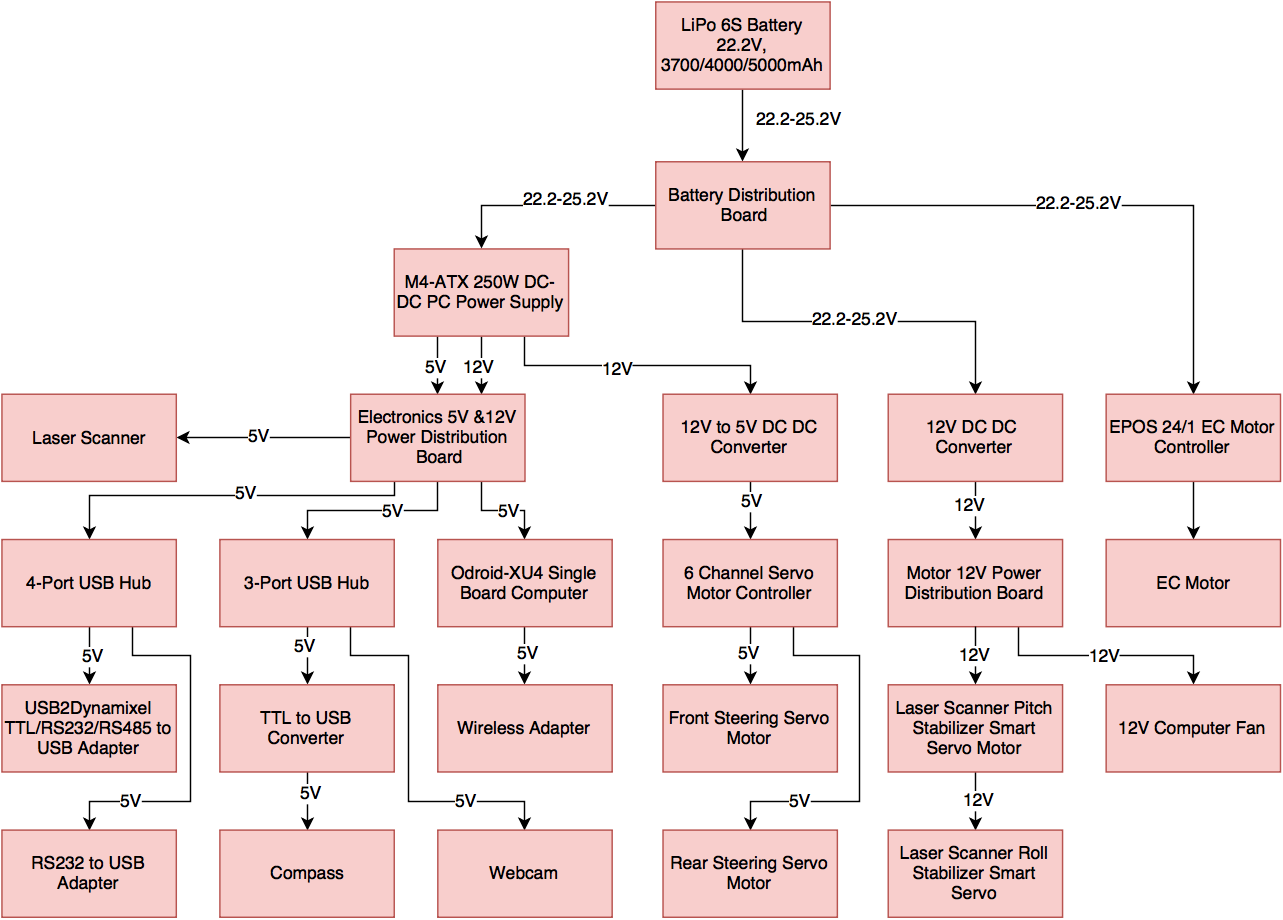
\includegraphics[width=0.9\linewidth]{Chapters/Chapter2/Figures/power_distribution.png}
	\caption{Σύστημα Τροφοδοσίας της ρομποτικής πλατφόρμας \textit{Monstertruck}.}
	\label{fig:power_distribution}
\end{figure}


%%%%%%%%%%%%%%%%%%%%%%%%%%%%%%%%%%%%%%%%%%%%%%%%%%%%%%%%%%%%%%%%%%%%%%%%%%%%%%%%%%%%%%%%%%%%%%
%%%%%%%%%%%%%%%%%%%%%%%%%%%%%%%%%%%%%%%%%%%%%%%%%%%%%%%%%%%%%%%%%%%%%%%%%%%%%%%%%%%%%%%%%%%%%%
%---------------------------------------------------------------------------------------------
%	SECTION 2: Motion Transfer System
%---------------------------------------------------------------------------------------------
\newpage
\section{Σύστημα Μετάδοσης Κίνησης} \label{sec:motion_transfer_system}
Ένα αυτοκίνητο όχημα, για να κινηθεί, απαιτεί την ύπαρξη {ενεργοποιητών(actuators)}, οι οποίοι μετατρέπουν την ενέργεια από μία πηγή τροφοδοσίας και ένα σήμα ελέγχου σε μηχανική κίνηση. Τον σκοπό αυτό, εξυπηρετούν οι κινητήρες και στην προκειμένη περίπτωση, για την επίτευξη της μηχανικής κίνησης του υλοποιημένου ρομποτικού οχήματος, χρησιμοποιούνται ένας κινητήρας, ο οποίος, μέσω ενός συστήματος μετάδοσης κίνησης, μεταδίδει την περιστροφική κίνηση του και στους τέσσερις τροχούς του οχήματος ({τετρακίνηση}) και δύο σερβοκινητήρες, οι οποίοι στρίβουν και τους τέσσερις τροχούς, με ανεξάρτητη στρέψη των μπροστινών, από τους πίσω τροχούς  ({τετραδιεύθυνση}). Στην συνέχεια, παρουσιάζεται η ανάλυση των μηχανισμών {τετρακίνησης} και {τετραδιεύθυνσης} της ρομποτικής πλατφόρμας {Monstertruck}.


\bigskip
\subsection{Σύστημα Τετρακίνησης} \label{ssec:four_wheel_drive}
Η μετάδοση της κίνησης, από τον μοναδικό κινητήρα του οχήματος, προς τους τέσσερις τροχούς, δηλαδή η τετρακίνηση επιτυγχάνεται, μέσω του {συστήματος μετάδοσης κίνησης (drivetrain)}, το οποίο παρουσιάζεται στο σχήμα \ref{fig:drivetrain}. Το σύστημα αυτό περιλαμβάνει, συνολικά, τέσσερα στάδια μετάδοσης της περιστροφικής κίνησης του κινητήρα, όπου κάθε στάδιο εισάγει ένα λόγο μείωσης των στροφών, αλλά ταυτόχρονα, αντίστροφο λόγο αύξησης της ροπής στρέψης.

\bigskip
\begin{figure}[!ht]
	\centering
	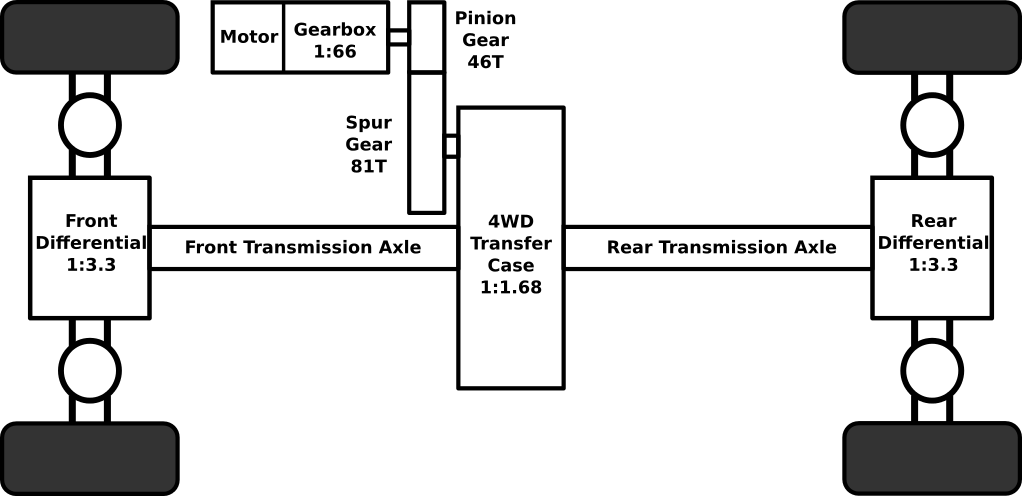
\includegraphics[width=0.8\linewidth]{Chapters/Chapter2/Figures/drivetrain.png}
	\caption{Σύστημα Μετάδοσης Κίνησης (Drivetrain) της ρομποτικής πλατφόρμας \textit{Monstertruck.}}
	\label{fig:drivetrain}
\end{figure}

\bigskip
Το πρώτο στάδιο μετάδοσης αποτελείται από το \textit{gearbox} του κινητήρα, το οποίο περιγράφεται από ένα λόγο μετάδοσης $\lambda_{gearbox}=1:66$. Ο λόγος, αυτός, μειώνει την μέγιστη περιστροφική ταχύτητα του κινητήρα, από $18\,000rpm$ σε $18\,000:66=272.72rpm$.

\bigskip
Το δεύτερο στάδιο μετάδοσης αποτελείται από δύο γρανάζια, το \textit{Πινιόν (Pinion Gear)} και \textit{Ώθησης (Spur Gear)}. Το {γρανάζι Πινιόν} μεταδίδει την κίνηση από τον κινητήρα στο {γρανάζι Ώθησης}, το οποίο με τη σειρά του μεταδίδει την κίνηση στο επόμενο στάδιο μετάδοσης. Το {γρανάζι Πινιόν} περιλαμβάνει $46$ οδοντώσεις, ενώ το {γρανάζι Ώθησης}, $81$, έχοντας ως αποτέλεσμα ένα λόγο μετάδοσης $\lambda_{spur\_pinion}=46:81=1:1.76$. Με την μείωση του δεύτερου σταδίου, η μέγιστη ταχύτητα μειώνεται στα $272.72:1.76 = 154.96rpm$.

\begin{figure}[!ht]
	\centering
	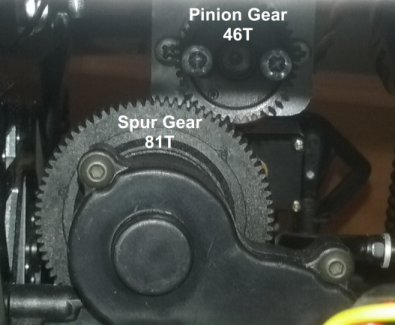
\includegraphics[width=0.4\linewidth]{Chapters/Chapter2/Figures/spur_and_pinion_gears.jpg}
	\caption{Γρανάζια Πινιόν και Ώθησης.}
	\label{fig:spur_pinion_gears}
\end{figure}

\bigskip
Το τρίτο στάδιο μετάδοσης και σημαντικότερο, για την επίτευξη {τετρακίνησης}, περιλαμβάνει το \textit{κιβώτιο μετάδοσης (Transfer Case)} του μπροστινού και του πίσω άξονα, που φαίνεται στο σχήμα \ref{fig:transfer_case}. Το {κιβώτιο μετάδοσης}, περιλαμβάνει δύο γρανάζια, το \textit{γρανάζι μετάδοσης (Transmission Gear)} και το \textit{διαφορικό γρανάζι (Differential Gear)}. Η περιστροφική κίνηση μεταδίδεται, από το {γρανάζι Ώθησης}, προς το {γρανάζι μετάδοσης}, μέσω ενός μηχανισμού \textit{σφιγκτήρα ολίσθησης (slipper clutch)}, που επιτρέπει την αποσύμπλεξη των γραναζιών, μέσω ολίσθησης, σε περίπτωση, υψηλής ροπής στους τροχούς, που θα μπορούσαν να προκαλέσουν ζημιά στα γρανάζια και στους άξονες μετάδοσης. Υπό φυσιολογικές συνθήκες, το {γρανάζι μετάδοσης}, μεταδίδει την περιστροφική κίνηση προς το {διαφορικό γρανάζι} και άρα και προς τους δύο άξονες μετάδοσης, με λόγο μετάδοσης $\lambda_{transfer\_case}=1:1.68$. Επομένως, έχουμε μία επιπλέον μείωση των στροφών, με αποτέλεσμα $154.96:1.68=92.24rpm$.

\begin{figure}[!ht]
	\centering
	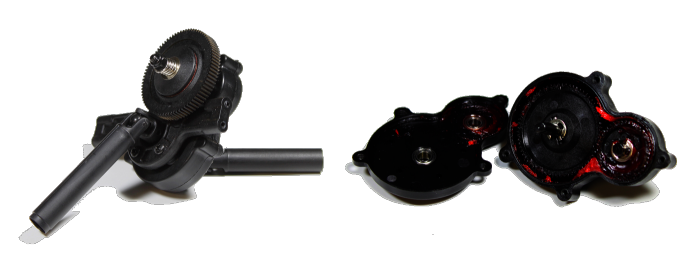
\includegraphics[width=0.8\linewidth]{Chapters/Chapter2/Figures/transfer_case.png}
	\caption{To κιβώτιο μετάδοσης κίνησης (Transfer Case) του οχήματος GroundPounder.}
	\label{fig:transfer_case}
\end{figure}

\bigskip
Το τέταρτο και τελευταίο στάδιο μετάδοσης της κίνησης, αποτελείται από δύο \textit{διαφορικά (differential)}, ένα για τους μπροστινούς τροχούς και ένα για τους πίσω. Το {διαφορικό} είναι ένας μηχανισμός, ο οποίος μετατρέπει την κατεύθυνση κίνησης, από την ευθύγραμμη, του άξονα μετάδοσης, στην εγκάρσια, των ημιαξόνων κάθε τροχού. Παράλληλα, επιτρέπει σε δύο τροχούς, έναν αριστερό και ένα δεξιό, να κινούνται με διαφορετική περιστροφική ταχύτητα ή ροπή, ανάλογα με την πρόσφυση σε κάθε έναν, από αυτούς. Ο μηχανισμός, αυτός, είναι απαραίτητος, καθώς, όταν ένα όχημα προσπαθεί να στρίψει, ακολουθώντας μία καμπύλη, οι τροχοί που βρίσκονται στην εξωτερική πλευρά της καμπύλης, διανύουν μεγαλύτερη απόσταση, από τους εσωτερικούς τροχούς και άρα θα πρέπει να κινούνται με μεγαλύτερη ταχύτητα. Τέλος, το κάθε {διαφορικό} εισάγει, ακόμη, έναν τελευταίο λόγο μείωσης των στροφών, της τάξης του $\lambda_{differential}=1:3.3$, οπότε η τελική μέγιστη ταχύτητα περιστροφής των τροχών προκύπτει $92.24:3.3=27.95rpm$.

\begin{figure}[!ht]
	\begin{minipage}{.49\textwidth}
		\centering
		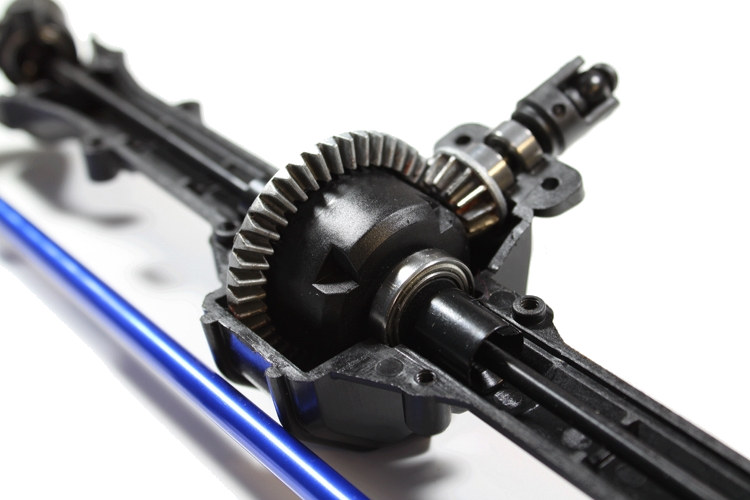
\includegraphics[width=0.5\linewidth]{Chapters/Chapter2/Figures/differential.png}
		\captionof{figure}{Το διαφορικό (Differential) του οχήματος GroundPounder.}
		\label{fig:differential}
	\end{minipage}
	\begin{minipage}{.5\textwidth}
	 	\centering		
		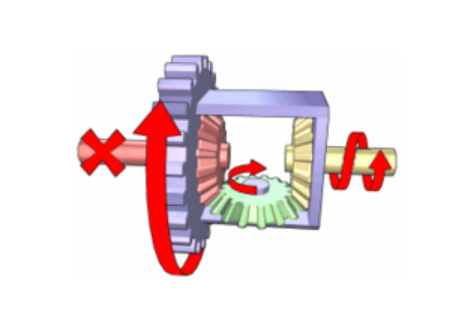
\includegraphics[width=0.5\linewidth]		
			{Chapters/Chapter2/Figures/differential_function.png}
		\captionof{figure}{Λειτουργία ενδεικτικού μηχανισμού διαφορικού.}
		\label{fig:differential_function}
	\end{minipage}
\end{figure}

\bigskip
Επομένως, η σχέση μετάδοσης της περιστροφικής ταχύτητας, από τον κινητήρα, στους τροχούς προκύπτει:

\begin{equation}
	\omega_{wheel} = \omega_{motor} / (\lambda_{gearbox} \times \lambda_{spur\_pinion} \times \lambda_{transfer\_case} \times \lambda_{differential}) = \omega_{motor} / 644
\end{equation}

\bigskip
\subsection{Σύστημα Τετραδιεύθυνσης} \label{ssec:four_wheel_steering}
Η ρομποτική πλατφόρμα {Monstertruck}, περιλαμβάνει δύο σερβοκινητήρες, υπεύθυνους για την ανεξάρτητη στρέψη των μπροστινών και πίσω τροχών. Η ανεξάρτητη αυτή στρέψη, επιτρέπει στο όχημα να λειτουργεί με μπροστινή στρέψη ({Μπροστινοδιεύθυνση ή FWS}), πίσω στρέψη ({Πίσωδιεύθυνση ή RWS}), ή ταυτόχρονη στρέψη ({Τετραδιεύθυνση ή 4WS}) των τροχών. Στην {τετραδιεύθυνση}, οι μπροστινοί τροχοί, μπορεί να στρίβουν, είτε, με την ίδια φορά με τους πίσω τροχούς, οπότε μιλάμε για \textbf{θετική τετραδιεύθυνση}, είτε με αντίθετη, οπότε μιλάμε για \textbf{αρνητική τετραδιεύθυνση}.

\bigskip
Εφόσον, υπάρχει ένας σερβοκινητήρας για τους μπροστινούς τροχούς και ένας για τους πίσω, γεννάται το ερώτημα, πώς μεταδίδεται η στρέψη από έναν σερβοκινητήρα σε δύο τροχούς, έναν αριστερό και έναν δεξιό. Ο μηχανισμός, που λύνει το πρόβλημα στην προκειμένη περίπτωση, ονομάζεται \textit{Μηχανισμός Στρέψης, μέσω Συνδέσμου Έλξης (Drag Link Steering Mechanism)}. Ο  μηχανισμός αυτός στην προκειμένη περίπτωση, όπως παρουσιάζεται και στο σχήμα \ref{fig:drag_link_steering}, αποτελείται από έναν σερβοκινητήρα, ένα \textit{μπράτσο Pitman (Pitman Arm)}, έναν \textit{σύνδεσμο έλξης (Drag Link)} και έναν \textit{σύνδεσμο ένωσης των τροχών (Tie Rod)}, όπως επίσης και τις \textit{αρθρώσεις στρέψης των τροχών (Wheel Steering Knuckles)}.

\begin{figure}[!ht]
	\centering
	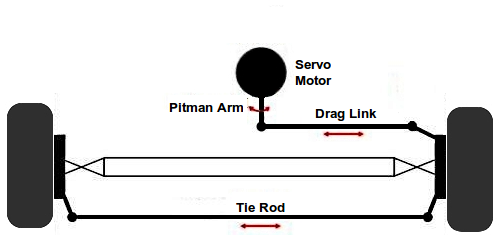
\includegraphics[width=0.6\linewidth]{Chapters/Chapter2/Figures/my_drag_link_steering.png}
	\caption{Ο Μηχανισμός στρέψης, με άξονα έλξης (Drag Link Steering Mechanism)
	\\της ρομποτικής πλατφόρμας Monstertruck.}
	\label{fig:drag_link_steering}
\end{figure}

\bigskip
Η περιστροφική κίνηση του σερβοκινητήρα, μεταδίδεται μέσω του {μπράτσου Pitman} και μετατρέπεται σε μεταφορική κίνηση του {συνδέσμου έλξης}, η οποία με τη σειρά της μετατρέπεται σε στρέψη της άρθρωσης του δεξιού τροχού. Η στρέψη, τώρα, της δεξιάς άρθρωσης, παρασύρει τον {σύνδεσμο ένωσης} των αρθρώσεων στρέψης των τροχών σε μεταφορική κίνηση, η οποία, έχει σαν αποτέλεσμα την στρέψη και του αριστερού τροχού. Ακολούθως, αναλύεται η λειτουργία του μηχανισμού στρέψης, σε δύο βήματα. Πρώτα υπολογίζεται η μετατόπιση $\Delta x$ του {συνδέσμου έλξης}, συναρτήσει της γωνίας στρέψης $\theta$ του σερβοκινητήρα και έπειτα, συναρτήσει της γωνίας στρέψης $\delta$ της άρθρωσης τροχού, με την οποία, είναι συνδεδεμένος ο {σύνδεσμος έλξης}.

\bigskip
\begin{figure}[!ht]
	\centering
	\subfloat[Ανάλυση για $\theta < 0$.]{
	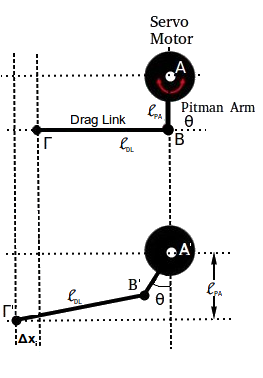
\includegraphics[width=0.4\linewidth]{Chapters/Chapter2/Figures/drag_link_analysis_1.png}
	\label{fig:drag_link_analysis_a}}
	\centering
	\subfloat[Ανάλυση για $\theta > 0$.]{
	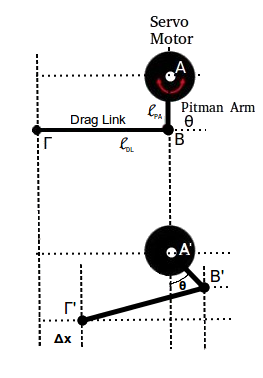
\includegraphics[width=0.4\linewidth]{Chapters/Chapter2/Figures/drag_link_analysis_2.png}
	\label{fig:drag_link_analysis_b}}
	\caption{Μετάδοση κίνησης από τον σερβοκινητήρα και το μπράτσο Pitman στον σύνδεσμο έλξης.}
	\label{fig:drag_link_analysis}	
\end{figure}

\bigskip
Λαμβάνοντας την παραδοχή, ότι η άκρη (σημείο Γ) του συνδέσμου έλξης, κινείται, μόνο οριζόντια και όχι κάθετα και με βάση το σχήμα \ref{fig:drag_link_analysis} και απλή γεωμετρική ανάλυση, μπορεί να εξαχθεί η  σχέση μεταξύ της γωνίας στρέψης $\theta$ του σερβοκινητήρα και της μετατόπισης $\Delta x$ του {συνδέσμου έλξης}, ως:

\begin{equation}
	\label{eq:drag_link_displacement}
	\Delta x =
	\begin{cases}
		\sqrt{l_{DL}^2 - l_{PA}^2(1-\cos(\theta))^2} + l_{PA} \sin(|\theta|) - l_{DL},  &\theta < 0\\ \\
	0, &\theta = 0\\ \\ 
	-\sqrt{l_{DL}^2 - l_{PA}^2(1-\cos(\theta))^2} - l_{PA} \sin(|\theta|) - l_{DL}, &\theta > 0
	\end{cases}
\end{equation}

\bigskip\noindent
όπου $l_{DL}$ είναι το μήκος του {συνδέσμου έλξης} και $l_{PA}$ είναι το μήκος του {μπράτσου Pitman}.

\begin{figure}[!ht]
	\centering
	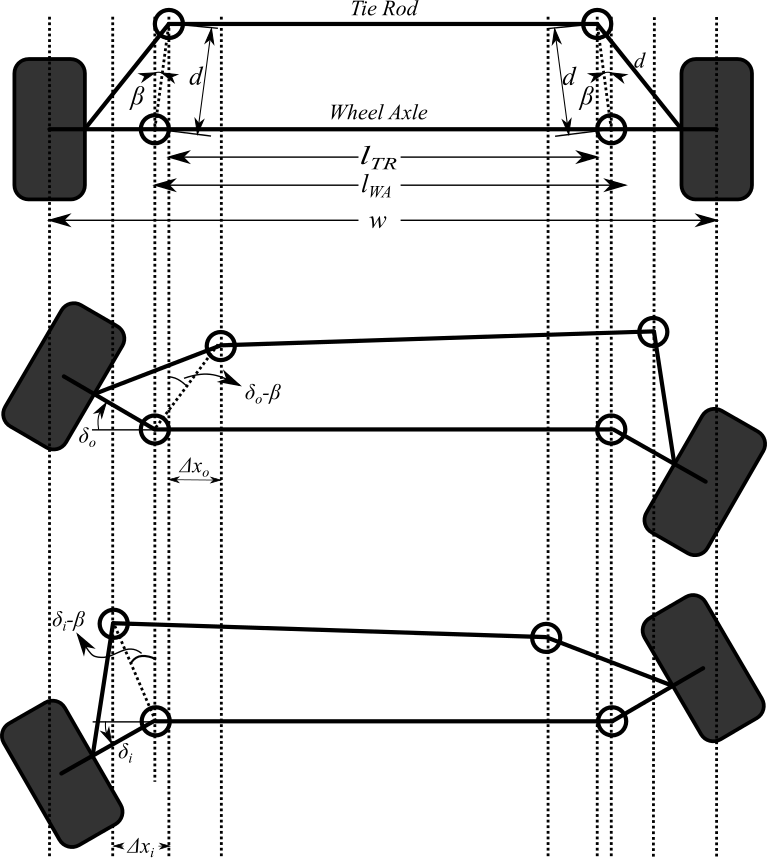
\includegraphics[width=0.8\linewidth]{Chapters/Chapter2/Figures/trapezoid_steering_mechanism.png}
	\caption{Τραπεζοειδής Μηχανισμός στρέψης των τροχών.}
	\label{fig:trapezoid_steering_mechanism}
\end{figure}

\bigskip
Με βάση το σχήμα \ref{fig:trapezoid_steering_mechanism}, μέσω γεωμετρικής ανάλυσης, προκύπτει ότι, η μετατόπιση του {συνδέσμου έλξης} $\Delta x$, συναρτήσει της γωνίας στρέψης, του άμεσα συνδεδεμένου τροχού, δηλαδή του αριστερού, στην προκειμένη περίπτωση, για τις περιπτώσεις, που ο τροχός είναι στην εσωτερική ή στην εξωτερική  πλευρά της στροφής, λαμβάνεται μέσω των ακόλουθων σχέσεων.
 
\begin{align}
	\label{eq:tie_rod_inner_displacement}
	\Delta x_i = d \sin(\delta_i - \beta) + d \sin(\beta)\\
	\label{eq:tie_rod_outer_displacement}\\
	\Delta x_o = d \sin(\delta_o + \beta) - d \sin(\beta)
\end{align}

\bigskip
Εξισώνοντας, τώρα, τις σχέσεις (\ref{eq:drag_link_displacement}), (\ref{eq:tie_rod_inner_displacement}), (\ref{eq:tie_rod_outer_displacement}), προκύπτει η σχέση μεταξύ της γωνίας στρέψης του σερβοκινητήρα και της γωνίας στρέψης του αριστερού τροχού, για τις περιπτώσεις που είναι εσωτερικά ($\delta_i$) στην στροφή και εξωτερικά ($\delta_o$):

\begin{equation}
	\label{eq:inner_steering_angle}
	\delta_i = \beta + \sin^{-1}{ \Bigg(
		\frac{
		\sqrt{l_{DL}^2 - l_{PA}^2(1-\cos(\theta))} + l_{PA} \sin{|\theta|} - l_{DL} - d \sin{\beta}}{d}} \Bigg)
\end{equation}

\begin{equation}
	\label{eq:outer_steering_angle}
	\delta_o = -\beta + \sin^{-1}{ \Bigg(
		\frac{
		-\sqrt{l_{DL}^2 - l_{PA}^2(1-\cos(\theta))} - l_{PA} \sin{|\theta|} - l_{DL} + d \sin{\beta}}{d}} \Bigg)
\end{equation}

\bigskip
Ο υπολογισμός της γωνίας στρέψης, του απέναντι τροχού, προκύπτει από τις εξισώσεις {τραπεζοειδούς μηχανισμού στρέψης τροχών} \cite{vehicle_dynamics}:

\begin{equation}
	\label{eq:trapezoid_steering_mechanism}
	sin(\beta + \delta_i) + sin(\beta - \delta_o) = \frac{L}{d} + \sqrt{\big(\frac{L}{d} - w \sin{\beta} \big)^2 - \big(\cos{(\beta-\delta_o)} - \cos{(\beta+\delta_i)}\big)^2}
\end{equation}

\bigskip
Αντικαθιστώντας την τιμή για την $\delta_i$, στην εξίσωση (\ref{eq:trapezoid_steering_mechanism}) θα πρέπει να εφαρμοστεί ένας επαναληπτικός αλγόριθμος, για την εύρεση της $\delta_o$ και αντίστροφα.

\bigskip
Για την απλοποίηση της όλης διαδικασίας μετατροπής της γωνίας στρέψης του σερβοκινητήρα, σε γωνίες στρέψης των τροχών και αντίστροφα, χρησιμοποιήθηκαν πολυωνυμικές προσεγγίσεις των σχέσεων μεταξύ αυτών, λύνοντας, επαναληπτικά και για όλες τις δυνατές τιμές, τις εξισώσεις (\ref{eq:inner_steering_angle}), (\ref{eq:outer_steering_angle}), (\ref{eq:trapezoid_steering_mechanism}) και για τις τιμές των παραμέτρων του μηχανισμού στρέψης που φαίνονται στον πίνακα \ref{tab:steering_parameter_values}.

\bigskip
\begin{table}[!ht]
	\centering
	\captionof{table}{Παράμετροι του μηχανισμού μετάδοσης στρέψης των τροχών,\\της ρομποτικής πλατφόρμας Monstertruck.}
	\begin{tabular}{| l | c |}
		\hline
		\textbf{Παράμετρος} & \textbf{Τιμή}\\ \hline
		$d$ & $30mm$ \\ \hline
		$\beta$ & $5^\circ$\\ \hline
		$l_{TR}$ & $225mm$\\ \hline
		$l_{WA}$ & $230mm$\\ \hline
		$l_{PA}$ & $20mm$\\ \hline
		$l_{DA}$ & $100mm$\\ \hline
	\end{tabular}
	\label{tab:steering_parameter_values}
\end{table}

\begin{align}
\begin{split}
\delta_{lf} &= 0.029\;\cdot \theta_{f}^2 + 0.6515\;\cdot \theta_{f} + 0.0006\\
\delta_{lr} &= 0.029\;\cdot \theta_{r}^2 + 0.6515\;\cdot \theta_{r} + 0.0006\\
\delta_{rf} &= -0.0058\;\cdot \delta_{lf}^2 + 1.0203\;\cdot \delta_{lf}\\
\delta_{rr} &= -0.0058\;\cdot \delta_{lr}^2 + 1.0203\;\cdot \delta_{lr}\\
\theta_{f}\, &= 0.1047\;\cdot \delta_{lf}^2 + 1.5362\;\cdot \delta_{lf} - 0.0009\\
\theta_{r}\, &= 0.1047\;\cdot \delta_{lr}^2 + 1.5362\;\cdot \delta_{lr} - 0.0009
\end{split}
\label{eq:polynoms}
\end{align}

\bigskip
\noindent
όπου

\begin{description}
	\item[\theta_{f}:] γωνία στρέψης του μπροστινού σερβοκινητήρα
	\item[\theta_{r}:] γωνία στρέψης του πίσω σερβοκινητήρα
	\item[\delta_{lf}:] γωνία στρέψης του μπροστινού αριστερού τροχού
	\item[\delta_{lr}:] γωνία στρέψης του πίσω αριστερού τροχού
	\item[\delta_{rf}:] γωνία στρέψης του μπροστινού δεξιού τροχού
	\item[\delta_{rr}:] γωνία στρέψης του πίσω δεξιού τροχού
\end{description}

%%%%%%%%%%%%%%%%%%%%%%%%%%%%%%%%%%%%%%%%%%%%%%%%%%%%%%%%%%%%%%%%%%%%%%%%%%%%%%%%%%%%%%%%%%%%%%
%%%%%%%%%%%%%%%%%%%%%%%%%%%%%%%%%%%%%%%%%%%%%%%%%%%%%%%%%%%%%%%%%%%%%%%%%%%%%%%%%%%%%%%%%%%%%%
%%%%%%%%%%%%%%%%%%%%%%%%%%%%%%%%%%%%%%%%%%%%%%%%%%%%%%%%%%%%%%%%%%%%%%%%%%%%%%%%%%%%%%%%%%%%%%

%----------------------------------------------------------------------------------------
%	SECTION 3: Kinematic Analysis
%----------------------------------------------------------------------------------------
\bigskip
\section{Κινηματική Ανάλυση} \label{sec:kinematic_analysis}
Ένα σύγχρονο αυτοκίνητο όχημα, στην πλειονότητα των περιπτώσεων, για να κινηθεί, περιλαμβάνει έναν κινητήρα, ο οποίος είναι υπεύθυνος για την περιστροφική κίνηση των μπροστινών (μπροστινοκίνηση), πίσω (πισωκίνηση) ή όλων (τετρακίνηση) των τροχών. Επίσης, περιλαμβάνει ένα σύστημα στρέψης των τροχών, είτε μπροστινών (μπροστινοδιεύθυνση), είτε πισινών (πισωδιεύθυνση), είτε και των τεσσάρων (τετραδιεύθυνση), έτσι ώστε να μπορεί να ακολουθεί καμπύλες τροχιές και όχι μόνο ευθύγραμμες. Η κινηματική ανάλυση του οχήματος, που παρουσιάζεται στην παρούσα ενότητα, προσπαθεί να περιγράψει την επίδραση του ελέγχου κίνησης των τροχών του, στην κίνηση του οχήματος και στις μεταβολές της {κατάστασης} του.

\bigskip
Η \textit{κατάσταση} ενός ρομποτικού οχήματος, συνήθως περιγράφεται από έξι μεταβλητές, τις καρτεσιανές συντεταγμένες του x, y, z, ως προς ένα αυθαίρετο εξωτερικό σύστημα συντεταγμένων και τις {γωνίες Euler yaw, pitch, roll}. Στην προκειμένη περίπτωση, το πρόβλημα που εξετάζεται, περιορίζεται σε επίπεδο περιβάλλον και επομένως, ως {κατάσταση} του οχήματος, λαμβάνεται, η \textit{πόζα} του $\mathbf{q}$, η οποία περιγράφεται από τις καρτεσιανές συνταγμένες του $x, y$ στο επίπεδο και τον προσανατολισμό του $\theta$, ως προς αυθαίρετο εξωτερικό σύστημα συντεταγμένων.

\begin{equation}
	\textbf{q} = [x\;\; y\;\; \theta]^T
	\label{eq:pose}
\end{equation}

\bigskip
Αντίστοιχα, η ταχύτητα ενός ρομποτικού οχήματος στο επίπεδο, ως προς ένα αυθαίρετο εξωτερικό σύστημα συντεταγμένων ορίζεται ως η μεταβολή της {πόζας} του $\mathbf{q}$, ως προς τον χρόνο.

\begin{equation}
	\dot{\mathbf{q}} = [\dot x\;\; \dot y\;\; \dot \theta]^T
	\label{eq:dpose}
\end{equation}

\bigskip
\noindent
Ενώ, η ταχύτητα ενός ρομποτικού οχήματος, στο επίπεδο, ως προς το κέντρο μάζας του $C$ είναι

\begin{equation}
	 \textbf{v} = [v_{cx}\;\; v_{cy}\;\; \omega_c]^T
	\label{eq:speed}
\end{equation}

\bigskip
\noindent
και αντιστοιχεί σε μία κυκλική τροχιά, ακτίνας $R$. Εφόσον, ένα διάνυσμα ταχυτήτων, αντιστοιχεί σε μία κυκλική τροχιά του κέντρου μάζας $C$ του οχήματος, τότε, μία επιθυμητή καμπύλη τροχιά, μπορεί να προσεγγιστεί, από ένα σύνολο τόξων κύκλου και τις αντίστοιχες  ταχύτητες τους.

\bigskip
\subsection{Κινηματικό Μοντέλο Ackermann} \label{ssec:ackermann_kinematics}
Το {Κινηματικό Μοντέλο \textit{Ackermann}, αποτελεί το δημοφιλέστερο και πιο διαδεδομένο κινηματικό μοντέλο στην αυτοκινητοβιομηχανία. Αναπτύχθηκε από τον Γερμανό μηχανικό Georg Lankensperger στο Μόναχο, το 1817, αλλά το δίπλωμα ευρεσιτεχνίας κατοχυρώθηκε από τον Rudolph Ackermann, το 1818, για ιππήλατες άμαξες. Τελικά, επεκτάθηκε και στην αυτοκινητοβιομηχανία και χρησιμοποιείται μέχρι και σήμερα.

\bigskip 
Σκοπός του κινηματικού μοντέλου {Ackermann} είναι η αποφυγή της πλευρικής ολίσθησης των τροχών, ενός τετράτροχου οχήματος κατά την ακολούθηση καμπύλων τροχιών. Για την εξυπηρέτηση αυτού του σκοπού, λοιπόν, το {κινηματικό μοντέλο Ackermann}, στηρίζεται σε μία συνθήκη, την λεγόμενη {συνθήκη Ackermann}, μεταξύ των τροχών στρέψης ενός οχήματος, που αν ικανοποιείται προβλέπει την κίνηση των τροχών χωρίς πλευρική ολίσθηση \cite{vehicle_dynamics}. Η συνθήκη Ackermann υποστηρίζει ότι για να κινείται ένα τετράτροχο όχημα χωρίς να ολισθαίνουν πλευρικά οι τροχοί του, θα πρέπει οι κάθετοι στους τροχούς άξονες να τέμνονται σε ένα κοινό σημείο, το οποίο ονομάζεται \textit{Στιγμιαίο Κέντρο Περιστροφής} (\textit{Instantaneous Center of Rotation - ICR}) \cite{4ws_kinematics} και αποτελεί το κέντρο της στιγμιαίας κυκλικής τροχιάς που ακολουθεί το όχημα.

\begin{figure}[!ht]
	\centering
	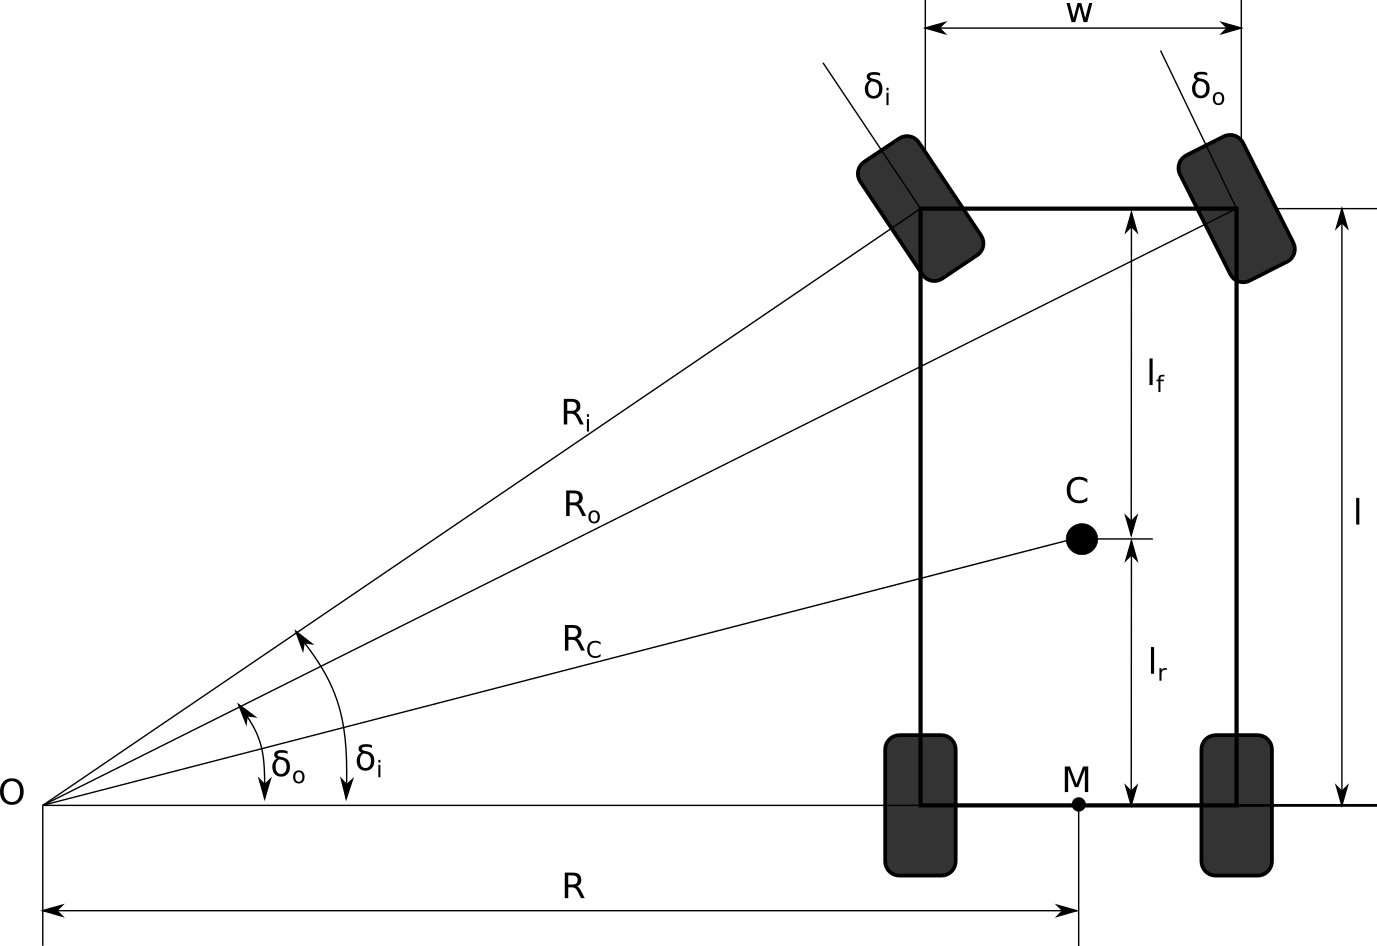
\includegraphics[width=0.7\linewidth]{Chapters/Chapter2/Figures/ackermann_model.png}
	\caption{Κινηματικό Μοντέλο Ackermann.}
	\label{fig:ackermann_model}
\end{figure}

\bigskip
Λαμβάνοντας υπόψιν το σχήμα \ref{fig:ackermann_model} προκύπτουν οι γωνίες στρέψης των τροχών ως

\begin{equation}
	\tan(\delta_i) = \frac{l}{R - \frac{w}{2}}
	\text{\;\;ή\;\;}	
	\cot(\delta_i) = \frac{R - \frac{w}{2}}{l}
	\label{eq:ackermann_inner_steering_angle}
\end{equation}

\begin{equation}
	\tan(\delta_o) = \frac{l}{R + \frac{w}{2}}
	\text{\;\;ή\;\;}
	\cot(\delta_o) = \frac{R + \frac{w}{2}}{l}
	\label{eq:ackermann_outer_steering_angle}
\end{equation}

Αφαιρώντας τις εξισώσεις (\ref{eq:ackermann_inner_steering_angle}), (\ref{eq:ackermann_outer_steering_angle}), προκύπτει η {συνθήκη Ackermann}.

\begin{equation}
	\cot{\delta_i} - \cot{\delta_o} = w / l
	\label{eq:ackermann_condition}
\end{equation}


\noindent
όπου
\begin{description}
	\item[\delta_i:] γωνία στρέψης εσωτερικού (inner), ως προς την στροφή, τροχού.
	\item[\delta_o:] γωνία στρέψης εξωτερικού (outer), ως προς την στροφή, τροχού.
	\item[l:] μεταξόνιο (wheelbase).
	\item[w:] μετατρόχιο (track).
	\item[R:] ακτίνα τροχιάς που εκτελεί το μεσαίο σημείο μεταξύ των πίσω τροχών.
\end{description}

\bigskip
Το όχημα, που παρουσιάζεται στο σχήμα \ref{fig:ackermann_model}, πραγματοποιεί μία κυκλική τροχιά γύρω από το {Στιγμιαίο Κέντρο Περιστροφής} Ο. Αν λάβοουμε ως σημείο αναφοράς το κέντρο του πίσω άξονα (σημείο $P$), τότε το όχημα εκτελεί μία κυκλική τροχιά, ακτίνας $R$, γύρω από το σημείο O. Η ακτίνα R, μπορεί να υπολογιστεί προσθέτοντας τις εξισώσεις (\ref{eq:ackermann_inner_steering_angle}), (\ref{eq:ackermann_outer_steering_angle}), ως

\begin{equation}
	R = l \cdot \frac{\cot{\delta_i} + \cot{\delta_o}}{2} = l \cot{\delta} = \frac{l}{\tan{\delta}}
	\label{eq:ackermann_rear_middle_turning_radius}
\end{equation}

\noindent
όπου $\delta$ είναι η γωνία στρέψης του ισοδύναμου κινηματικού μοντέλου ποδηλάτου (σχήμα \ref{fig:ackermann_bicylce_model}). 

\begin{figure}[!ht]
	\centering
	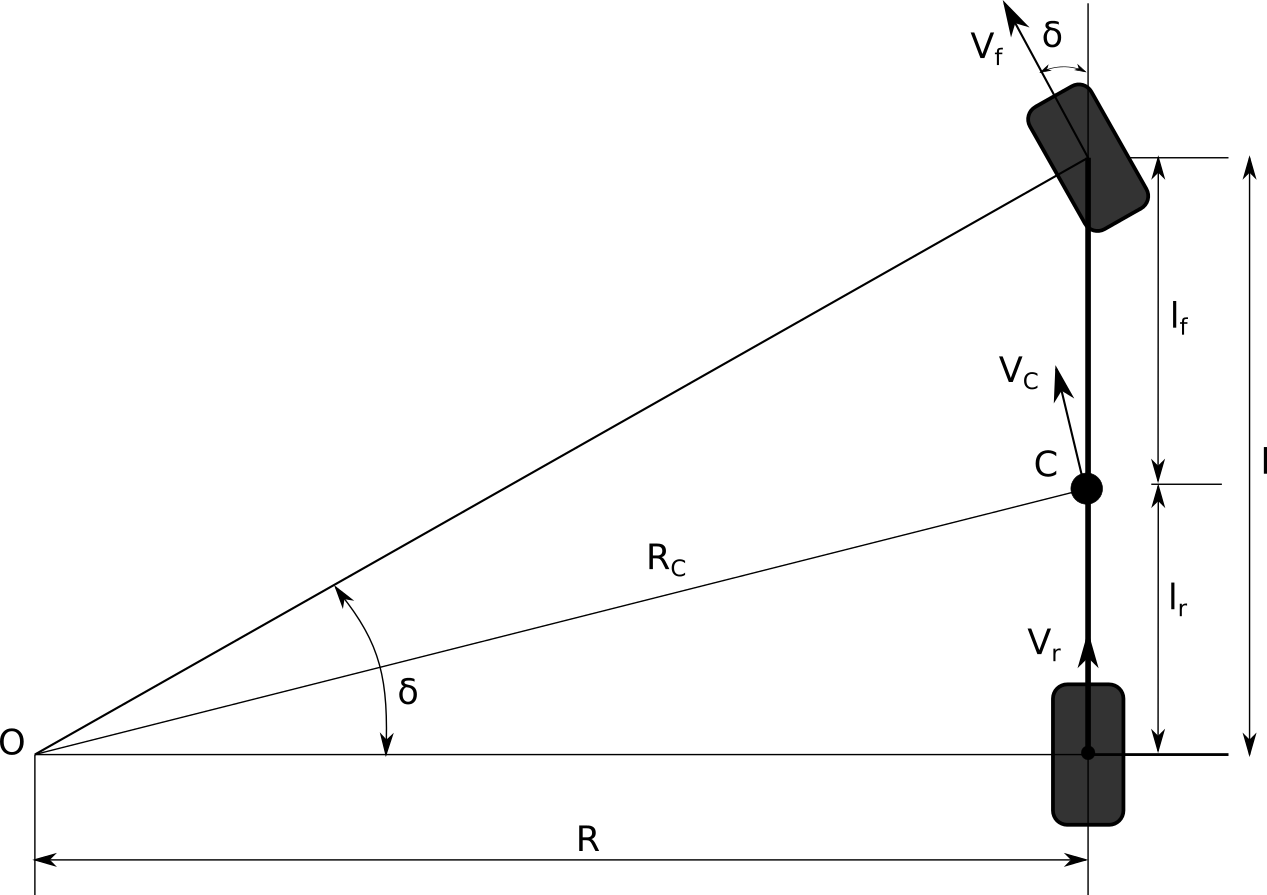
\includegraphics[width=0.6\linewidth]{Chapters/Chapter2/Figures/ackermann_bicycle_model.png}
	\caption{Ισοδύναμο μοντέλο ποδηλάτου Ackermann.}
	\label{fig:ackermann_bicylce_model}
\end{figure}

\bigskip
Αντίστοιχα, ο υπολογισμός της ακτίνας $R_c$ του κέντρου μάζας του οχήματος, με βάση το σχήμα \ref{fig:ackermann_model}, προκύπτει 

\begin{equation}
	R_c = \sqrt{R^2 + l_R^2} = \sqrt{R^2 + (l - l_F)^2}
	\label{eq:ackermann_center_mass_turning_radius}
\end{equation}

\noindent
όπου, $l_R$ και $l_F$ είναι η απόσταση του κέντρου μάζας του οχήματος από τον άξονα των μπροστινών και πίσω τροχών αντίστοιχα, όπου $l_R + l_F = l$.

\bigskip
Κατά την κίνηση σε κυκλική τροχιά, κάθε τροχός του οχήματος διαγράφει διαφορετική τροχιά από τους υπόλοιπους. Για παράδειγμα, στο σχήμα \ref{fig:ackermann_model}, για να καταστεί δυνατή η εκτέλεση της τροχιάς, γύρω από το Ο, χωρίς ολίσθηση, θα πρέπει οι τροχοί να κινούνται με ίδια γωνιακή ταχύτητα $\dot\theta$, ως προς το κέντρο $O$ και με διαφορετική γραμμική ταχύτητα, και άρα, καθένας, να περιστρέφεται με διαφορετική περιστροφική ταχύτητα $\omega$, ανάλογη της ακτίνας της τροχιάς που διαγράφει. Επομένως, ισχύει

\begin{equation}
	\dot\theta_{ir} = \dot\theta_{or} = \dot\theta_{if} = \dot\theta_{of} = \dot\theta
	\label{eq:theta_dot}
\end{equation}

\bigskip
\noindent
και αντικαθιστώντας στην εξίσωση (\ref{eq:theta_dot}), την σχέση μεταξύ γωνιακής και γραμμικής ταχύτητας
	
\begin{equation}
	v = \dot\theta \cdot R
	\label{eq:v_theta}
\end{equation}	

\noindent
η εξίσωση (\ref{eq:theta_dot}) μετασχηματίζεται στη μορφή
	
\begin{equation}	
	\frac{v_{ir}}{R_{ir}} = \frac{v_{or}}{R_{or}} = \frac{v_{if}}{R_{if}} = \frac{v_{of}}{R_{of}} = \dot\theta = \frac{v_c}{R_c}
	\label{eq:theta_dot_2}
\end{equation}

\noindent
όπου
\begin{description}
	\item[ir:] εσωτερικός πίσω τροχός
	\item[or:] εξωτερικός πίσω τροχός
	\item[if:] εσωτερικός μπροστινός τροχός
	\item[of:] εξωτερικός μπροστινός τροχός
\end{description}

\bigskip
Επομένως, με βάση τις δύο παραπάνω παρατηρήσεις, και την σχέση (\ref{eq:theta_dot_2}) μπορεί να υπολογιστεί η γραμμική ταχύτητα κάθε τροχού, ως

\begin{align}
	v_{if} &= \dot\theta \cdot R_{if} = \dot\theta \cdot \sqrt{l^2 + (R - \frac{w}{2})^2}
	\label{eq:ack_vif}\\
	v_{of} &= \dot\theta \cdot R_{of} = \dot\theta \cdot \sqrt{l^2 + (R + \frac{w}{2})^2}
	\label{eq:ack_vof}\\
	v_{ir} &= \dot\theta \cdot R_{ir} = \dot\theta \cdot (R - \frac{w}{2})
	\label{eq:ack_vir}\\
	v_{or} &= \dot\theta \cdot R_{or} = \dot\theta \cdot (R + \frac{w}{2})
	\label{eq:ack_vor}
\end{align}

\bigskip
Χρησιμοποιώντας, τις εξισώσεις (\ref{eq:ack_vif}) - (\ref{eq:ack_vor}), όπως επίσης και την σχέση μεταξύ γραμμικής ταχύτητας $v$, περιστροφικής ταχύτητας $\omega$ και ακτίνας τροχού $r$
\begin{equation}
	v = \omega \cdot r
	\label{eq:v_omega}
\end{equation}

\noindent
προκύπτουν οι περιστροφικές ταχύτητες των τροχών, ως

\begin{align}
	\omega_{ir} &= \frac{\dot\theta}{r} \cdot R_{ir} = \frac{\dot\theta}{r} \cdot (R - \frac{w}{2})
	\label{eq:ack_wir}\\
	\omega_{or} &= \frac{\dot\theta}{r} \cdot R_{or} = \frac{\dot\theta}{r} \cdot (R + \frac{w}{2})
	\label{eq:ack_wor}\\
	\omega_{if} &= \frac{\dot\theta}{r} \cdot R_{if} = \frac{\dot\theta}{r} \cdot \sqrt{l^2 + (R - \frac{w}{2})^2}
	\label{eq:ack_wif}\\
	\omega_{of} &= \frac{\dot\theta}{r} \cdot R_{of} = \frac{\dot\theta}{r} \cdot \sqrt{l^2 + (R + \frac{w}{2})^2}
	\label{eq:ack_wof}
\end{align}

\bigskip
Τέλος, οι ταχύτητες του κέντρου του άξονα των πίσω τροχών, ως προς ένα αυθαίρετο εξωτερικό σύστημα συντεταγμένων, βάση του \textit{ισοδύναμου κινηματικού μοντέλου ποδηλάτου Ackermann}, είναι:

\begin{align}
	\dot X_r &= v_r \cdot \cos\theta\\
	\dot Y_r &= v_r \cdot \sin\theta\\
	\dot \Theta_r &= \frac{v_r}{l} \cdot \tan\delta
\end{align}

Ενώ, οι ταχύτητες του κέντρου του άξονα των μπροστινών τροχών, ως προς ένα αυθαίρετο εξωτερικό σύστημα συντεταγμένων, είναι:

\begin{align}
	\dot X_f &= v_f \cdot \cos(\theta+\delta)\\
	\dot Y_f &= v_f \cdot \sin(\theta+\delta)\\
	\dot \Theta_f &= \frac{v_f \cdot \sin\delta}{l}
\end{align}


%%%%%%%%%%%%%%%%%%%%%%%%%%%%%%%%%%%%%%%%%%%%%%%%%%%%%%%%%%%%%%%%%%%%%%%%%%%%%%%%%%%%%%%%%%%%%%
\bigskip
\subsection{Κινηματικό Μοντέλο Τετραδιεύθυνσης} \label{ssec:4ws_kinematics}
Το \textit{κινηματικό μοντέλο τετραδιεύθυνσης} αποτελεί επέκταση του {κινηματικού μοντέλου Ackermann}, χρησιμοποιώντας, ταυτόχρονη στρέψη των μπροστινών και πίσω τροχών του οχήματος. Προσφέρει, με αυτόν τον τρόπο μεγαλύτερη ευελιξία, μέσω μειωμένης ακτίνας τροχιάς , συγκριτικά με το απλό {μοντέλο Ackermann} $(R_{4WS, min} < R_{2WS, min})$, ενώ, ακόμα, παρέχει και δυνατότητα  διαγώνιας κίνησης, μέσω παράλληλης στρέψης των τροχών (crab steering). Επίσης, στην ειδική περίπτωση, που κάθε τροχός, μπορεί να κινηθεί και να στραφεί ανεξάρτητα από τους άλλους, το όχημα μπορεί να πραγματοποιήσει επί τόπου στροφή (0-point-turn, $R_{min}=0$), κάτι που δεν εφαρμόζεται στην ρομποτική πλατφόρμα {Monstertruck}.

\bigskip
Στην παρούσα ενότητα, θα μας απασχολήσει η κινηματική ανάλυση του \textit{μοντέλου τετραδιεύθυνσης}, για τις λειτουργίες, της {αρνητικής στρέψης (negative/counter steering)} και της {θετικής στρέψης (positive/crab steering)} των τροχών. Η \textit{αρνητική τετραδιεύθυνση}, χρησιμοποιείται σε αυτοκίνητα, για χαμηλές ταχύτητες ($< 40 km/h$), με στόχο την αυξημένη ευελιξία, μέσω πραγματοποίησης πιο στενών ελιγμών. Αντίθετα, η \textit{θετική τετραδιεύθυνση}, χρησιμοποιείται για, υψηλές ταχύτητες ($> 40 km/h$), για πιο ομαλή αλλαγή λωρίδων, μέσω πιο μικρών μεταβολών στην ακτίνα της τροχιάς που εκτελεί. Σε ρομποτικές εφαρμογές, όπως και η παρούσα, όπου οι ταχύτητες είναι πολύ μικρότερες, το μοντέλο θετικής στρέψης μπορεί να χρησιμοποιηθεί σε αλγορίθμους κατασκευής μονοπατιών, για την επέκταση του ρεπερτορίου των δυνατών κινήσεων, αλλά και για την ενίσχυση αλγορίθμων διάσχισης μονοπατιού, μέσω διόρθωσης απόκλισης, σε περιπτώσεις παρεκκλίνουσας συμπεριφοράς, λόγω εξωτερικών παραγόντων, όπως ολίσθηση, ή ατελειών του κινηματικού ή του δυναμικού μοντέλου του οχήματος. Επίσης, στην ειδική περίπτωση {θετικής τετραδιεύθυνσης}, όπου οι πίσω τροχοί στρέφονται με την ίδια γωνία και φορά με τους μπροστινούς, το όχημα κινείται πλαγίως, με μηδενική γωνιακή ταχύτητα και άρα μηδενική μεταβολή προσανατολισμού.


\bigskip
Η κινηματική ανάλυση του {μοντέλου τετραδιεύθυνσης}, ακολουθεί ίδια κατεύθυνση με την κινηματική ανάλυση του {μοντέλου Ackermann}, μέσω μία αντίστοιχης συνθήκης στρέψης των τροχών (steering condition) \cite{vehicle_dynamics}. Η συνθήκη αυτή, την οποία θα καλούμε, \textit{συνθήκη τετραδιεύθυνσης}, ορίζει την σχέση μεταξύ των γωνιών στρέψης και των τεσσάρων τροχών, έτσι ώστε, οι, κάθετοι στους τροχούς, άξονες να τέμνονται σε ένα κοινό σημείο (σχήματα \ref{fig:4ws_model}, \ref{fig:pos_4ws_model}). 

\bigskip
Η ανάλυση του {κινηματικού μοντέλου τετραδιεύθυνσης} και η εξαγωγή των εξισώσεων και σχέσεων, που ακολουθεί στην συνέχεια, χρησιμοποιεί την διάταξη {αρνητικής τετραδιεύθυνσης}, που παρουσιάζεται στο σχήμα \ref{fig:4ws_model}, αλλά ισχύει, παράλληλα και για την διάταξη {θετικής τετραδιεύθυνσης}, γεγονός που μπορεί να αποδειχθεί με απλή γεωμετρική ανάλυση του σχήματος \ref{fig:pos_4ws_model}.

\begin{figure}[!ht]
	\centering
	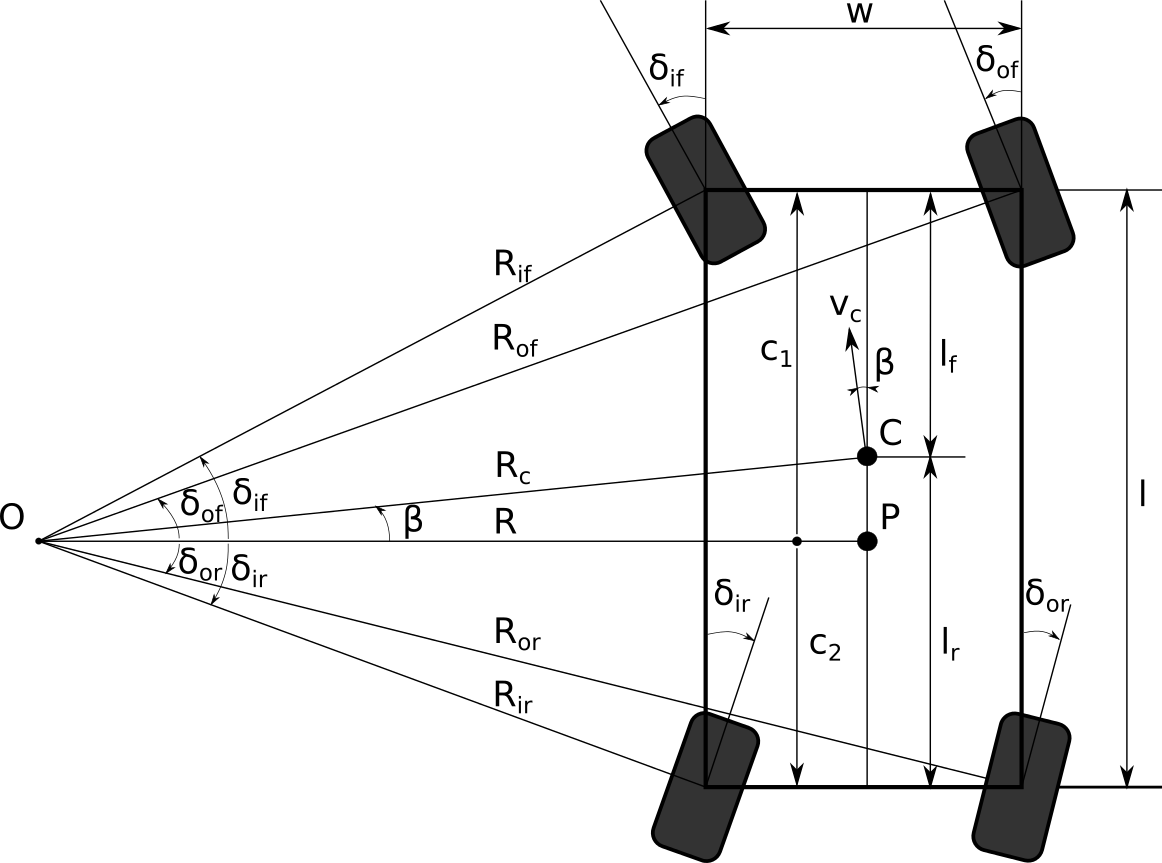
\includegraphics[width=0.7\linewidth]{Chapters/Chapter2/Figures/4ws_model.png}
	\caption{Κινηματικό μοντέλο αρνητικής τετραδιεύθυνσης.}
	\label{fig:4ws_model}
\end{figure}

\begin{figure}[!ht]
	\centering
	\includegraphics[width=0.7\linewidth]{Chapters/Chapter2/Figures/pos_4ws_model.png}
	\caption{Κινηματικό μοντέλο θετικής τετραδιεύθυνσης.}
	\label{fig:pos_4ws_model}
\end{figure}

\bigskip
Μέσω γεωμετρικής ανάλυσης του σχήματος \ref{fig:4ws_model}, βάση του ορισμού της {συνθήκης τετραδιεύθυνσης}, προκύπτουν οι γωνίες στρέψης των τροχών του οχήματος:

\begin{align}
	\tan{\delta_{if}} &= \frac{c_1}{R-\frac{w}{2}}
	\label{eq:4ws_front_inner_steering_angle}\\
	\tan{\delta_{of}} &= \frac{c_1}{R+\frac{w}{2}}
	\label{eq:4ws_front_outer_steering_angle}\\
	\tan{\delta_{ir}} &= \frac{c_2}{R-\frac{w}{2}}
	\label{eq:4ws_rear_inner_steering_angle}\\
	\tan{\delta_{or}} &= \frac{c_2}{R+\frac{w}{2}}
	\label{eq:4ws_rear_outer_steering_angle}		
\end{align}

Aντιστρέφοντας και αφαιρώντας τις σχέσεις (\ref{eq:4ws_front_inner_steering_angle}), (\ref{eq:4ws_front_outer_steering_angle}) και (\ref{eq:4ws_rear_inner_steering_angle}), (\ref{eq:4ws_rear_outer_steering_angle}) προκύπτουν οι συνθήκες τετραδιεύθυνσης των μπροστινών και πίσω τροχών, αντίστοιχα.

\begin{align}
	\cot{\delta_{of}} - \cot{\delta_{if}} &= \frac{w}{c_1}
	\label{eq:front_4ws_condition}\\
	\cot{\delta_{or}} - \cot{\delta_{ir}} &= \frac{w}{c_2}
	\label{eq:rear_4ws_condition}
\end{align}

\noindent
Έπειτα, προσθέτοντας τις προκύπτουσες εξισώσεις (\ref{eq:front_4ws_condition}), (\ref{eq:rear_4ws_condition}), λαμβάνεται η μαθηματική εξίσωση της \textit{συνθήκης τετραδιεύθυνσης}.

\begin{equation}
	\frac{1}{\cot{\delta_{of}} - \cot{\delta_{if}}} + \frac{1}{\cot{\delta_{or}} - \cot{\delta_{ir}}} = \frac{c_1 - c_2}{w} = \frac{l}{w}
	\label{eq:4ws_condition}
\end{equation}


\bigskip\bigskip
H γωνία $\beta$ πλευρικής ολίσθησης (sideslip angle) \cite{automated_odometry} του κέντρου μάζας $\,C\,$ του οχήματος, υπολογίζεται, εύκολα, από το ισοδύναμο \textit{μοντέλο ποδηλάτου τετραδιεύθυνσης} (σχήμα \ref{fig:4ws_bicycle}).

\begin{equation}
	\tan{\beta} = \frac{l_r \cdot \tan{\delta_f} + l_f \cdot \tan{\delta_r}}{l}
	\label{eq:neg_4ws_beta}\\
\end{equation} 

\noindent
όπου
\begin{description}
	\item[\delta_f:] γωνία στρέψης μπροστινού τροχού ισοδύναμου μοντέλου ποδηλάτου τετραδιεύθυνσης
	\item[\delta_r:] γωνία στρέψης πίσω τροχού ισοδύναμου μοντέλου ποδηλάτου τετραδιεύθυνσης
\end{description}

\bigskip
Οι γωνίες στρέψης $\delta_f$ και $\delta_r$, μπορούν να υπολογιστούν για ένα όχημα με \textit{τετραδιεύθυνση} ως

\begin{align}
	\cot{\delta_f} &= \frac{\cot{\delta_{if}} + \cot{\delta_{of}}}{2} = \frac{R}{c_1}
	\label{eq:df}\\
	\cot{\delta_r} &= \frac{\cot{\delta_{ir}} + \cot{\delta_{or}}}{2} = \frac{R}{c_2}
	\label{eq:dr}
\end{align}

\bigskip
Αντιστρέφοντας και αφαιρώντας τις εξισώσεις (\ref{eq:dr}), (\ref{eq:df}), υπολογίζεται η ακτίνα $R$ της τροχιάς του σημείου $P$

\begin{equation}
	R = \frac{l}{\tan{\delta_f} - \tan{\delta_r}}
	\label{eq:pos_p_turning_radius}
\end{equation}


\bigskip
\noindent
και έπειτα η ακτίνα $R_c$ της τροχιάς του κέντρου μάζας $C$ του οχήματος.

\begin{equation}
	R_c = \frac{R}{\cos{\beta}} = \frac{l}{\cos{\beta} \cdot (\tan{\delta_f} - \tan{\delta_r})}
\end{equation}

\begin{figure}[!ht]
	\centering
	\includegraphics[width=0.6\linewidth]{Chapters/Chapter2/Figures/4ws_bicycle.png}
	\caption{Ισοδύναμο μοντέλο ποδηλάτου αρνητικής τετραδιεύθυνσης.}
	\label{fig:4ws_bicycle}
\end{figure}

\begin{figure}[!ht]
	\centering
	\includegraphics[width=0.6\linewidth]{Chapters/Chapter2/Figures/pos_4ws_bicycle_model.png}
	\caption{Ισοδύναμο μοντέλο ποδηλάτου θετικής τετραδιεύθυνσης.}
	\label{fig:pos_4ws_bicycle_model}
\end{figure}

\bigskip
Για τον υπολογισμό των ταχυτήτων θα χρησιμοποιηθούν και πάλι, οι εξισώσεις (\ref{eq:theta_dot})-(\ref{eq:theta_dot_2}), εφόσον ισχύουν και στην προκειμένη περίπτωση, σε συνδυασμό με τις σχέσεις των ακτίνων τροχιάς κάθε τροχού, όπως προκύπτει από το σχήμα \ref{fig:4ws_model}.

\begin{align}
	R_{if} &= \frac{R - \frac{w}{2}}{\cos{\delta_{if}}}
	\label{eq:neg_4ws_rif}\\
	R_{of} &= \frac{R + \frac{w}{2}}{\cos{\delta_{of}}}
	\label{eq:neg_4ws_rof}\\
	R_{ir} &= \frac{R - \frac{w}{2}}{\cos{\delta_{ir}}}
	\label{eq:neg_4ws_rir}\\
	R_{or} &= \frac{R + \frac{w}{2}}{\cos{\delta_{or}}}
	\label{eq:neg_4ws_or}
\end{align}

\bigskip
Επομένως, οι γραμμικές ταχύτητες των τροχών προκύπτουν, ως

\begin{align}
	\label{eq:neg_4ws_vif}	
	v_{if} &= \dot\theta \cdot R_{if} = \frac{v_c}{R_c} \cdot \frac{R - \frac{w}{2}}{\cos{\delta_{if}}}\\
	\label{eq:neg_4ws_vof}	
	v_{of} &= \dot\theta \cdot R_{of} = \frac{v_c}{R_c} \cdot \frac{R + \frac{w}{2}}{\cos{\delta_{of}}}\\
	\label{eq:neg_4ws_vir}	
	v_{ir} &= \dot\theta \cdot R_{ir} = \frac{v_c}{R_c} \cdot \frac{R - \frac{w}{2}}{\cos{\delta_{ir}}} \\
	\label{eq:neg_4ws_vor}
	v_{or} &= \dot\theta \cdot R_{or} = \frac{v_c}{R_c} \cdot \frac{R + \frac{w}{2}}{\cos{\delta_{or}}}
\end{align}

\bigskip
\noindent
και αντίστοιχα οι περιστροφικές ταχύτητες των τροχών, με βάση την εξίσωση (\ref{eq:v_omega}), προκύπτουν

\begin{align}
	\label{eq:neg_4ws_wif}	
	\omega_{if} &= \frac{v_{if}}{r} = \frac{v_c}{r \cdot R_c} \cdot \frac{R - \frac{w}{2}}{\cos{\delta_{if}}}\\
	\label{eq:neg_4ws_wof}	
	\omega_{of} &= \frac{v_{if}}{r} = \frac{v_c}{r \cdot R_c} \cdot \frac{R + \frac{w}{2}}{\cos{\delta_{of}}}\\
	\label{eq:neg_4ws_wir}	
	\omega_{ir} &= \frac{v_{if}}{r} = \frac{v_c}{r \cdot R_c} \cdot \frac{R - \frac{w}{2}}{\cos{\delta_{ir}}} \\
	\label{eq:neg_4ws_wor}
	\omega_{or} &= \frac{v_{if}}{r} = \frac{v_c}{r \cdot R_c} \cdot \frac{R + \frac{w}{2}}{\cos{\delta_{or}}}
\end{align} 

\bigskip
Με βάση την παραπάνω κινηματική ανάλυση, οι εξισώσεις των ταχυτήτων, του οχήματος, ως προς το κέντρο μάζας του \textit{C}, μπορούν να υπολογιστούν, χρησιμοποιώντας τις σχέσεις

\begin{equation}
	\tan{\beta} = \frac{v_{c,y}}{v_{c,x}} \;\;\Leftrightarrow\;\; v_{c,y} = v_{c,x} \cdot \tan{\beta}
	\label{eq:vel_beta}
\end{equation}
\begin{equation}
	v_c^2 = v_{c,x}^2 + v_{c,y}^2 \;\;\Leftrightarrow\;\; v_{c}^2 = v_{c,x}^2 - v_{c,x}^2  \cdot \tan^2{\beta}
	\label{eq:v_squared}
\end{equation}
\begin{equation}
	v_c = \omega_c \cdot R_c
	\label{eq:lin_ang_relationship}
\end{equation}

\noindent
από τις οποίες, τελικά προκύπτουν οι εξισώσεις των ταχυτήτων του οχήματος, ως προς το κέντρο μάζας του $C$:

\begin{align}
	v_{c,x} &= \frac{v_c}{\sqrt{1+\tan^2\beta}}
	\label{eq:lin_vel_x}\\
	v_{c,y} &= \frac{v_c \cdot \tan{\beta}}{\sqrt{1+\tan^2\beta}}
	\label{eq:lin_vel_y}\\
	\omega_c &= \frac{v_c \cdot \cos{\beta} \cdot (\tan{\delta_f - \tan{\delta_r}})}{l}
	\label{eq:ang_vel}
\end{align}

\bigskip\noindent
όπου
\begin{description}
	\item[v_c:] η συνισταμένη γραμμική ταχύτητα του κέντρου μάζας του οχήματος
	\item[v_{c,x}:] η γραμμική επιμήκης ταχύτητα του κέντρου μάζας του οχήματος
	\item[v_{c,y}:] η γραμμική εγκάρσια ταχύτητα του κέντρου μάζας του οχήματος
	\item[\omega_c:] η γωνιακή ταχύτητα του κέντρου μάζας του οχήματος
\end{description}

\bigskip\bigskip
Τέλος, οι ταχύτητες κέντρου μάζας $C$ του οχήματος, ως προς ένα αυθαίρετο εξωτερικό σύστημα συντεταγμένων, προκύπτουν βάση του \textit{ισοδύναμου κινηματικού μοντέλου ποδηλάτου τετραδιεύθυνσης} (σχήμα \ref{fig:4ws_bicycle}) \cite{4ws_trajectory_planning}.

\begin{align}
	\dot X &= v_c \cdot \cos(\theta + \beta)
	\label{eq:x_dot}\\
	\dot Y &= v_c \cdot \sin(\theta + \beta)
	\label{eq:y_dot}\\
	\dot \Theta &= \omega_c = \frac{v_c \cdot \cos{\beta} \cdot (\tan{\delta_f - \tan{\delta_r}})}{l}
	\label{eq:th_dot}
\end{align}

\noindent
όπου,
\begin{equation}
	v_c = \frac{v_f \cdot \cos{\delta_f} + v_r \cos{\delta_r}}{2 \cdot \cos{\beta}}
	\label{eq:v_c_f_r}
\end{equation}

\begin{figure}[!ht]
	\centering
	\includegraphics[width=0.6\linewidth]{Chapters/Chapter2/Figures/4ws_xy_plane.png}
	\caption[Ισοδύναμο κινηματικό μοντέλο ποδηλάτου τετραδιεύθυνσης στο επίπεδο ΧΥ.]{Ισοδύναμο κινηματικό μοντέλο ποδηλάτου τετραδιεύθυνσης στο επίπεδο ΧΥ \cite{4ws_trajectory_planning}.}
	\label{fig:4ws_xy_plane}
\end{figure}

%%%%%%%%%%%%%%%%%%%%%%%%%%%%%%%%%%%%%%%%%%%%%%%%%%%%%%%%%%%%%%%%%%%%%%%%%%%%%%%%%%%%%%%%%%%%%%
%%%%%%%%%%%%%%%%%%%%%%%%%%%%%%%%%%%%%%%%%%%%%%%%%%%%%%%%%%%%%%%%%%%%%%%%%%%%%%%%%%%%%%%%%%%%%%
\newpage
\bigskip
\subsection{Κινηματικό Μοντέλο Ρομποτικής Πλατφόρμας \textit{Monstertruck}} \label{ssec:monstertruck_kinematics}
Η ρομποτική πλατφόρμα {Monstertruck} περιλαμβάνει ένα {μη ιδανικό κινηματικό μοντέλο τετραδιεύθυνσης}, με την έννοια, ότι δεν υπακούει στην {συνθήκη τετραδιεύθυνσης} (\ref{eq:4ws_condition}). Το γεγονός αυτό, οφείλεται στο μηχανισμό μετάδοσης της στρέψης των τροχών που παρουσιάστηκε στην ενότητα \ref{ssec:four_wheel_steering} και ο οποίος ορίζει μία σχέση, μεταξύ εσωτερικού και εξωτερικού τροχού, με αρκετά μεγάλη απόκλιση από την ιδανική συνθήκη τετραδιεύθυνσης \ref{eq:4ws_condition}, ή ακόμα και από την ιδανική συνθήκη Ackermann \ref{eq:ackermann_condition} όπως παρουσιάζεται και στο σχήμα \ref{fig:steer_angles_comparison}.

\begin{figure}[!ht]
	\centering
	\includegraphics[width=0.6\linewidth]{Chapters/Chapter2/Figures/steer_angles_comparison.png}
	\caption{Η σχέση στρέψης μεταξύ εσωτερικού και εξωτερικού τροχού για τα κινηματικά μοντέλα \\Ackermann, Τετραδιεύθυνσης και της ρομποτικής πλατφόρμας Monstertruck.}
	\label{fig:steer_angles_comparison}
\end{figure}

Εφόσον, παραβιάζεται η {συνθήκη τετραδιεύθυνσης} (\ref{eq:4ws_condition}), η κίνηση της ρομποτικής πλατφόρμας {Monstertruck}, θα επιβαρύνεται από πλευρική ολίσθηση των τροχών. Παρόλα αυτά, επειδή, η ρομποτική πλατφόρμα, σχεδιάστηκε και προορίζεται για εφαρμογές εξαιρετικά μικρών ταχυτήτων και επομένως τυχόν δυναμικά φαινόμενα, που παρουσιάζονται, κατά την κίνηση, είναι αμελητέα, η κίνηση της ρομποτικής πλατφόρμας, μπορεί να προσεγγισθεί από το {ιδανικό κινηματικό μοντέλο τετραδιεύθυνσης}. 

\bigskip
Για την κινηματική ανάλυση του μοντέλου της ρομποτικής πλατφόρμας {Monstertruck}, θα χρησιμοποιήσουμε τις παραδοχές, ότι η διαφορά της γωνίας στρέψης μεταξύ δεξιού και αριστερού τροχού είναι αμελητέα και ότι σε χαμηλές ταχύτητες, η κίνηση της ρομποτικής πλατφόρμας, περιγράφεται, με αμελητέο σφάλμα, από τις εξισώσεις κίνησης του κινηματικού μοντέλου {τετραδιεύθυνσης} στο επίπεδο.

\bigskip
Το {μη ιδανικό κινηματικό μοντέλο τετραδιεύθυνσης} της ρομποτικής πλατφόρμας {Monstertruck}, παρουσιάζεται στο σχήμα \ref{fig:monstetruck_model}. Στο μοντέλο αυτό, το {Στιγμιαίο Κέντρο Περιστροφής Ο}, βρίσκεται στην τομή των κάθετων στους τροχούς, αξόνων του {ισοδύναμου κινηματικού μοντέλου ποδηλάτου τετραδιεύθυνσης}. Σαν αποτέλεσμα η διεύθυνση κάθε τροχού είναι διάφορη της διεύθυνσης της ταχύτητας του κατά μία γωνία $\alpha$, που ονομάζεται \textit{γωνία πλευρικής ολίσθησης τροχού (side slip angle)} \cite{4ws_kinematics}, όπως παρουσιάζεται στο σχήμα \ref{fig:monstertruck_slip_angle_model}.


\begin{figure}[!ht]
	\centering
	\includegraphics[width=0.7\linewidth]{Chapters/Chapter2/Figures/monstertruck_model_parallel.png}
	\caption{Το κινηματικό μοντέλο της ρομποτικής πλατφόρμας Monstertruck,\\ σε διάταξη αρνητικής τετραδιεύθυνσης.}
	\label{fig:monstetruck_model}
\end{figure}

\bigskip
Με βάση το μη ιδανικό μοντέλο τετραδιεύθυνσης, που παρουσιάζεται στο σχήμα \ref{fig:monstertruck_slip_angle_model}, ο εσωτερικός τροχός στρέφεται κατά ίδια γωνία με τον αντίστοιχο εξωτερικό. Παρόλα αυτά, επειδή το όχημα, εκτελεί μία περιστροφική κίνηση, γύρω από το $O$, οι εξωτερικοί τροχοί διανύουν μεγαλύτερη απόσταση από τους εσωτερικούς, το οποίο σημαίνει ότι οι τροχοί ολισθαίνουν. Οι γωνίες της συνισταμένης ταχύτητας των τροχών δίνονται από τις ακόλουθες σχέσεις.

\begin{align}
	\cot(\delta_{if} + \alpha_{if}) = \frac{R - \frac{w}{2}}{c_1}
	\label{eq:monst_dif}\\
	\cot(\delta_{of} - \alpha_{of}) = \frac{R + \frac{w}{2}}{c_1}
	\label{eq:monst_dof}\\
	\cot(\delta_{ir} + \alpha_{ir}) = \frac{R - \frac{w}{2}}{c_2} 
	\label{eq:monst_dir}\\
	\cot(\delta_{or} - \alpha_{or}) = \frac{R + \frac{w}{2}}{c_2}
	\label{eq:monst_dor}
\end{align}


\begin{figure}[!ht]
	\centering
	\includegraphics[width=0.7\linewidth]{Chapters/Chapter2/Figures/monstertruck_slip_angle_model_parallel.png}
	\caption{Το μη ιδανικό κινηματικό μοντέλο τετραδιεύθυνσης, με πλευρική ολίσθηση τροχών,\\ της ρομποτικής πλατφόρμας Monstertruck, σε διάταξη αρνητικής τετραδιεύθυνσης.}
	\label{fig:monstertruck_slip_angle_model}
\end{figure}

\bigskip
Αφαιρώντας τις (\ref{eq:monst_dif}), (\ref{eq:monst_dof}) και (\ref{eq:monst_dif}), (\ref{eq:monst_dof}) προκύπτουν οι σχέσεις τετραδιεύθυνσης του μη ιδανικού μοντέλου, για τους μπροστινούς και πίσω τροχούς.

\begin{align}
	\cot(\delta_{of} - \alpha_{of}) - \cot(\delta_{if} + \alpha_{if}) = \frac{w}{c1}
	\label{eq:monst_front_condition}\\
	\cot(\delta_{or} - \alpha_{or}) - \cot(\delta_{ir} + \alpha_{ir}) = \frac{w}{c2}
	\label{eq:monst_rear_condition}\\
\end{align}

\bigskip
Έπειτα, αντιστρέφοντας και αφαιρώντας τις σχέσεις (\ref{eq:monst_front_condition}), (\ref{eq:monst_rear_condition}) προκύπτει τελικά, η {κινηματική συνθήκη του μη ιδανικού μοντέλου τετραδιεύθυνσης της ρομποτικής πλατφόρμας Monstertruck} \cite{4ws_kinematics}. 

\begin{equation}
	\frac{1}{\cot(\delta_{of} - \alpha_{of}) - \cot(\delta_{if} + \alpha_{if})} - \frac{1}{\cot(\delta_{or} - \alpha_{or}) - \cot(\delta_{ir} + \alpha_{ir})} = \frac{c_1 - c_2}{w} = \frac{l}{w}
	\label{eq:monst_kinematic_condition}
\end{equation}

\bigskip
Με βάση την παραδοχή, ότι το όχημα περιστρέφεται με συνισταμένη γραμμική ταχύτητα $v_c$ και γωνιακή ταχύτητα $\omega_c$, γύρω από το κέντρο $O$, υπολογίζονται αρχικά οι ακτίνες περιστροφής των τροχών γύρω από το κέντρο $O$.

\begin{align}
	R_{if} = \frac{R_c}{\cos(\delta_{if} + \alpha_{if})}
	\label{eq:monst_rif}\\
	R_{of} = \frac{R_c}{\cos(\delta_{of} - \alpha_{of})}
	\label{eq:monst_rof}\\
	R_{ir} = \frac{R_c}{\cos(\delta_{ir} + \alpha_{ir})}
	\label{eq:monst_rir}\\
	R_{or} = \frac{R_c}{\cos(\delta_{or} - \alpha_{or})}
	\label{eq:monst_ror}
\end{align}

\bigskip
Έπειτα, μπορούμε να υπολογίσουμε τις συνισταμένες ταχύτητες κάθε τροχού γύρω από το κέντρο $O$, χρησιμοποιώντας την αντίστοιχη ακτίνα τροχιάς.

\begin{align}
	\label{eq:monst_vif}	
	v_{if} &= \dot\theta \cdot R_{if} = \frac{v_c}{R_c} \cdot \frac{R - \frac{w}{2}}{\cos(\delta_{if} - \alpha_{if})}\\
	\label{eq:monst_vof}	
	v_{of} &= \dot\theta \cdot R_{of} = \frac{v_c}{R_c} \cdot \frac{R + \frac{w}{2}}{\cos(\delta_{of} - \alpha_{of})}\\
	\label{eq:monst_vir}	
	v_{ir} &= \dot\theta \cdot R_{ir} = \frac{v_c}{R_c} \cdot \frac{R - \frac{w}{2}}{\cos(\delta_{ir} + \alpha_{ir})} \\
	\label{eq:monst_vor}
	v_{or} &= \dot\theta \cdot R_{or} = \frac{v_c}{R_c} \cdot \frac{R + \frac{w}{2}}{\cos(\delta_{or} - \alpha_{or})}
\end{align}

Επομένως, με βάση τις συνισταμένες ταχύτητες $v$ και τις γωνίες πλευρικής ολίσθησης $\alpha$, (σχήμα \ref{fig:slip_angles})μπορούμε να υπολογίσουμε τις επιμήκεις ταχύτητες των τροχών ως

\begin{align}
	\label{eq:monst_vifx}	
	v_{if,x} &= \frac{v_{if}}{\cos\alpha_{if}}\\
	\label{eq:monst_vofx}	
	v_{of,x} &= \frac{v_{of}}{\cos\alpha_{of}} \\
	\label{eq:monst_virx}	
	v_{ir,x} &= \frac{v_{ir}}{\cos\alpha_{ir}} \\
	\label{eq:monst_vorx}
	v_{or,x} &= \frac{v_{or}}{\cos\alpha_{or}}
\end{align}

\begin{figure}[!ht]
   \centering
	\includegraphics[width=0.35\linewidth]{Chapters/Chapter2/Figures/slip_angles.png}
	\caption{Ολίσθηση τροχών, λόγω μη ιδανικού μηχανισμού στρέψης.}
	\label{fig:slip_angles}
\end{figure}


\bigskip
Τέλος, οι περιστροφικές ταχύτητες των τροχών, υπολογίζονται από τις ακόλουθες σχέσεις

\begin{align}
	\label{eq:monst_wif}	
	\omega_{if} &= \frac{v_{if,x}}{r} = \frac{v_c \cdot (R - \frac{w}{2})}{r \cdot R_c \cdot \cos\alpha_{if} \cdot \cos(\delta_{if} - \alpha_{if})}\\
	\label{eq:monst_wof}
	\omega_{of} &= \frac{v_{of,x}}{r} = \frac{v_c \cdot (R + \frac{w}{2})}{r \cdot R_c \cdot \cos\alpha_{of} \cdot \cos(\delta_{of} - \alpha_{of})}\\
	\label{eq:monst_wir}	
	\omega_{ir} &= \frac{v_{ir,x}}{r} = \frac{v_c \cdot (R - \frac{w}{2})}{r \cdot R_c \cdot \cos\alpha_{ir} \cdot \cos(\delta_{ir} - \alpha_{ir})}\\
	\label{eq:monst_wor}
	\omega_{or} &= \frac{v_{or,x}}{r} = \frac{v_c \cdot (R + \frac{w}{2})}{r \cdot R_c \cdot \cos\alpha_{or} \cdot \cos(\delta_{or} - \alpha_{or})}
\end{align}

\bigskip
Οι παραπάνω τύποι, μπορούν να χρησιμοποιηθούν και για διαφορετικά κινηματικά μοντέλα {τετραδιεύθυνσης}, αντικαθιστώντας κατάλληλα τις γωνίες στρέψης $\delta$ και τις γωνίες πλευρικής ολίσθησης $\alpha$. Επίσης, περιγράφουν και το ιδανικό κινηματικό μοντέλο {τετραδιεύθυνσης} για μηδενικές γωνίες πλευρικής ολίσθησης $\alpha$ των τροχών και για γωνίες στρέψης $\delta$ που υπακούν στις εξισώσεις  (\ref{eq:4ws_front_inner_steering_angle})-(\ref{eq:4ws_rear_outer_steering_angle}).

\bigskip
Για τις γωνίες στρέψης της ρομποτικής πλατφόρμας Monstertruck, με βάση την παραδοχή της αμελητέας διαφοράς στρέψης, ισχύουν οι ακόλουθες εξισώσεις.

\begin{align}
	\delta_{if} = \delta_{of} = \delta_{f}
	\label{eq:monst_front_angles}\\
	\delta_{ir} = \delta_{or} = \delta_{r}
	\label{eq:monst_rear_angles}
\end{align}

Επομένως, οι γωνίες πλευρικής ολίσθησης των τροχών προκύπτουν ως

\begin{align}
	\alpha_{if} &= \tan^{-1}(\frac{c_1}{R-\frac{w}{2}}) - \delta_f
	\label{eq:monst_aif}\\
	\alpha_{of} &= -\tan^{-1}(\frac{c_1}{R+\frac{w}{2}}) + \delta_f
	\label{eq:monst_aof}\\
	\alpha_{ir} &= \tan^{-1}(\frac{c_2}{R-\frac{w}{2}}) - \delta_r
	\label{eq:monst_air}\\
	\alpha_{or} &= -\tan^{-1}(\frac{c_2}{R+\frac{w}{2}}) + \delta_r
	\label{eq:monst_aor}	
\end{align}


Τέλος, οι ταχύτητες του κέντρου μάζας C του οχήματος, ως προς ένα αυθαίρετο σύστημα συντεταγμένων, υπολογίζονται από τους τύπους του ιδανικού κινηματικού μοντέλου τετραδιεύθυνσης (\ref{eq:x_dot})-(\ref{eq:th_dot}).


%% Chapter Template

\chapter{Αυτόνομη Πλοήγηση σε Άγνωστο Περιβάλλον} % Main chapter title
\label{Chapter3} % Change X to a consecutive number; for referencing this chapter elsewhere, use \ref{ChapterX}

Στο παρόν κεφάλαιο θα παρουσιαστούν μέθοδοι και αλγόριθμοι που χρησιμοποιήθηκαν στη ρομποτική πλατφόρμα Monstertruck, για να καταστεί δυνατή η αυτόνομη πλοήγηση της σε ένα άγνωστο περιβάλλον. Θα μας απασχολήσουν θέματα σχετικά με τον εντοπισμό της θέσης του ρομποτικού οχήματος στον χώρο και την χαρτογράφηση του χώρου αυτού, μέσω μετρήσεων από τους αισθητήρες του ρομπότ αλλά και την ασφαλή και κινηματικά εφικτή αυτόνομη πλοήγηση μέσα σε αυτόν, αποσκοπώντας στην άφιξη σε έναν δεδομένο στόχο, ή την πλήρη εξερεύνηση του χώρου.

%----------------------------------------------------------------------------------------
%	SECTION 1: State Estimation, Mapping and SLAM
%----------------------------------------------------------------------------------------
\section{Εντοπισμός Θέσης και Χαρτογράφηση} \label{sec:localization_and_mapping}
Κατά την αυτόνομη πλοήγηση, ένα ρομποτικό όχημα θα πρέπει να γνωρίζει την θέση και τον προσανατολισμό του, δηλαδή την \textit{πόζα} του, ως προς ένα συγκεκριμένο αδρανειακό πλαίσιο. Το πρόβλημα εντοπισμού θέσης (localization), συνήθως λύνεται βάσει ενός συνόλου μεθόδων που παρέχουν πληροφορία, σχετικά με την πόζα του ρομπότ. Η πληροφορία αυτή μπορεί να είναι είτε \textit{απόλυτη}(global localization), είτε \textit{σχετική} (local localization) \cite{autonomous_land_vehicles}. Για παράδειγμα, αισθητήρες GPS, παρέχουν απόλυτη πληροφορία για την πόζα ενός ρομποτικού οχήματος, με βάση ορόσημα (landmarks). Αντίθετα, αισθητήρες, που μετρούν ταχύτητες ή ανιχνεύουν οπτικά χαρακτηριστικά στο περιβάλλον, παρέχουν μία σχετική πληροφορία της νέας πόζας του ρομποτικού οχήματος, ως προς την προηγούμενη.

\bigskip
Συνήθως, στις σύγχρονες ρομποτικές εφαρμογές, χρησιμοποιείται πληθώρα αισθητήρων και άρα πηγών πληροφορίας, είτε σχετική, είτε απόλυτη, σχετικά με την πόζα του ρομποτικού οχήματος και επομένως απαιτούνται μέθοδοι συνδυασμού και συγχώνευσης της πληροφορίας από όλες τις πηγές, για την παραγωγή μίας πιο αξιόπιστης εκτίμησης της κατάστασης του. Για την εξυπηρέτηση του σκοπού αυτού, ιδιαίτερα δημοφιλή λύση, αποτελεί η χρήση πιθανοτικών μεθόδων, όπως τα {Φίλτρα Kalman}, ο {Εντοπισμός Θέσης Markov} ({Markov Localization}) και \textit{Monte Carlo} ({Monte Carlo Localization}).

\bigskip
Για να μπορεί ένα ρομπότ να ξέρει ανά πάσα στιγμή την θέση του και να μπορεί να πλοηγηθεί σε ένα άγνωστο περιβάλλον για να φτάσει σε κάποιον στόχο, αποφεύγοντας, ταυτόχρονα, τυχόν εμπόδια, θα πρέπει να διαθέτει μία μέθοδο χαρτογράφησης του περιβάλλοντος του. Επομένως, η χαρτογράφηση αποτελεί μία απαραίτητη ικανότητα για κάθε αυτόνομο ρομπότ, που προορίζεται για χρήση σε άγνωστο περιβάλλον. Μία αξιόπιστη μέθοδος χαρτογράφησης, όμως, προϋποθέτει και μία αποδοτική και εύρωστη μέθοδο εντοπισμού θέσεις. Γι αυτό το λόγο, υπάρχει το ευρέως μελετημένο αντικείμενο αλγορίθμων {Ταυτόχρονης Χαρτογράφησης και Εντοπισμού Θέσης} ({SLAM}).

\bigskip
\subsection{Οδομετρία} \label{ssec:odometry}
%--------------------%
Η Οδομετρία είναι μία μέθοδος υπολογισμού της μεταβολής της {πόζας} ενός ρομποτικού οχήματος. Οι πιο δημοφιλείς μέθοδοι οδομετρίας, σε ρομποτικές εφαρμογές, είναι η {οδομετρία τροχών (wheel odometry)} και η {οπτική οδομετρία (visual odometry)}. Η {οδομετρία τροχών} χρησιμοποιεί τις μετρήσεις των ταχυτήτων των τροχών ενός ρομποτικού οχήματος για την εξαγωγή των ταχυτήτων αυτού και μέσω ολοκλήρωσης των ταχυτήτων, υπολογίζει την μεταβολή της πόζας του οχήματος. Αντίστοιχα, η {οπτική οδομετρία}, χρησιμοποιεί μία κάμερα για τον υπολογισμό της μεταβολής της πόζας του οχήματος, μέσω των μεταβολών, μεταξύ διαδοχικών εικόνων. Στην προκειμένη περίπτωση, παρόλα αυτά, θα μας απασχολήσει μόνο η περίπτωση της {οδομετρίας τροχών}.

\bigskip
Η {οδομετρία τροχών} απαιτεί την μέτρηση της ταχύτητας κάθε τροχού και με βάση το κινηματικό μοντέλο την εξαγωγή των ταχυτήτων του οχήματος. Παρόλα αυτά, η ρομποτική πλατφόρμα {Monstetruck}, δεν περιλαμβάνει ξεχωριστούς κινητήρες και αισθητήρες μέτρησης ταχύτητας για κάθε τροχό, αλλά μόνο έναν κινητήρα του συστήματος {τετρακίνησης}, που μεταδίδει την κίνηση και στους τέσσερις τροχούς. Επομένως, θα λάβουμε την παραδοχή, ότι οι ταχύτητες κάθε τροχού υπακούν στις εξισώσεις (\ref{eq:monst_vif})-(\ref{eq:monst_vor}) του κινηματικού μοντέλου της ρομποτικής πλατφόρμας {Monstertruck}, με βάση την μέτρηση της ταχύτητας που παρέχει ο εν λόγω κινητήρας.

\bigskip
Η γραμμική ταχύτητα του οχήματος προκύπτει από την μέτρηση της ταχύτητας του κινητήρα, ως
\begin{equation}
	v_c = \frac{\omega_{motor}}{644 \cdot r}
\end{equation}

\bigskip\noindent
ενώ  οι γωνίες στρέψης $\delta_{lf}, \delta_{rf}, \delta_{lr}, \delta_{rr}$ των τροχών, υπολογίζονται από τις γωνίες στρέψεις των σερβοκινητήρων και τις σχέσεις (\ref{eq:polynoms}).

\bigskip
Με βάση τις γωνίες στρέψης των τροχών, μπορούμε να υπολογίσουμε τις γωνίες στρέψης $\delta_f, \delta_r$ του {ισοδύναμου κινηματικού μοντέλου ποδηλάτου τετραδιεύθυνσης}, μέσω των τύπων  (\ref{eq:df}),(\ref{eq:dr}) και, επομένως, την γωνία πλευρικής ολίσθησης $\beta$ του κέντρου μάζας $C$ του οχήματος, βάσει του τύπου (\ref{eq:neg_4ws_beta}).

\bigskip
Έπειτα, μέσω της γωνίας πλευρικής ολίσθησης $\beta$, των γωνιών στρέψης $\delta_f, \delta_r$ και της συνισταμένης γραμμικής ταχύτητας του κέντρου μάζας $C$ του οχήματος $v_c$, μπορούμε να υπολογίσουμε τις συνιστώσες της γραμμική ταχύτητας $v_x, v_y$, αλλά και την γωνιακή ταχύτητα $\omega_c$ του οχήματος, μέσω των τύπων (\ref{eq:lin_vel_x})-(\ref{eq:ang_vel}).

\bigskip
Με βάση τους K. Bohlmann et al. \cite{automated_odometry}, μέσω γεωμετρικής προσέγγισης των κυκλικών τροχιών για μικρά διαστήματα Δt, ως γραμμικές τροχιές, η νέα πόζα του οχήματος, μπορεί να υπολογιστεί, σε σχέση με την προηγούμενη, βάσει των ακόλουθων τύπων.

\begin{align}
	X_{i} &= X_{i-1} + \Delta d \cdot \cos(\Theta_{i-1} + \frac{\Delta\Theta}{2} + \beta_{i-1} + \frac{\Delta\beta}{2})\\
	Y_{i} &= Y_{i-1} + \Delta d \cdot \sin(\Theta_{i-1} + \frac{\Delta\Theta}{2} + \beta_{i-1} + \frac{\Delta\beta}{2})\\
	\Theta_{i} &= \Theta_{i-1} + \Delta\Theta
\end{align}

\noindent
όπου
\begin{align}
	\Delta d &= v_c \cdot \Delta T\\
	\Delta\Theta &= \omega_c \cdot \Delta T
\end{align}

\bigskip
Τέλος, το γενικό πρόβλημα με την οδομετρία έγκειται στην ολοκλήρωση των ταχυτήτων, όπου, λόγω, ολίσθησης, σφαλμάτων μετρήσεων και ατελειών κινηματικού ή δυναμικού μοντέλου, εισάγεται ολοκληρωτικό σφάλμα που αυξάνεται όλο και περισσότερο με το πέρασμα του χρόνου. Το γεγονός αυτό, καθιστά την μέθοδο της οδομετρίας τροχών, ανεπαρκή ως αυτοτελή μέθοδο εντοπισμού θέσης.

\bigskip
Πολλές φορές παράλληλα, με την οδομετρία τροχών χρησιμοποιούνται και αισθητήρες κατεύθυνσης (πυξίδα, IMU), που μπορεί να παρέχουν μετρήσεις της γωνιακής ταχύτητας, γραμμικής επιτάχυνσης και απόλυτου προσανατολισμού ως προς τους άξονες x,y,z.

\bigskip
Στην ρομποτική πλατφόρμα {Monstertruck}, όπως προαναφέρθηκε στην ενότητα \ref{ssec:electronic_equipment}, χρησιμοποιείται μία πυξίδα {Compass OS4000}, που διαθέτει μαγνητόμετρο και επιταχυνσιόμετρο και άρα παρέχει πληροφορία για τον απόλυτο προσανατολισμό $yaw, pitch, roll$ και την γραμμική επιτάχυνση $a_x, a_y, a_z$, ως προς τους άξονες x,y,z. Επίσης, οι γραμμικές επιταχύνσεις, μπορούν να ολοκληρωθούν, για τον υπολογισμό της μεταβολής των γραμμικών ταχυτήτων $u_x, u_y, u_z$ του οχήματος, ενώ με δεύτερη ολοκλήρωση, για τον υπολογισμό της μεταβολής της θέσης $X, Y, Z$. Παρόλα αυτά, οι εν λόγω μετρήσεις, δεν είναι αρκετά αξιόπιστες και είναι επιρρεπείς σε συσσωρευτικά σφάλματα, λόγω ολοκλήρωσης.

\bigskip
Οι μετρήσεις της πυξίδας, μπορούν να χρησιμοποιηθούν, συμπληρωματικά με τις μετρήσεις της {οδομετρίας τροχών}, με στόχο την εξαγωγή της πλήρους κατάστασης $q = [x, y, z, roll, pitch, yaw]$  του οχήματος και τον πιο αξιόπιστο εντοπισμό θέσης, σε περίπτωση φαινομένων ολίσθησης των τροχών.

\bigskip
\subsection{Εκτίμηση Κατάστασης με Συνδυαστική Αντίληψη} 
\label{ssec:state_estimation_and_sensor_fusion}
Για την εκτίμηση της \textit{κατάστασης} ενός ρομπότ, μπορούν να χρησιμοποιηθούν μία πληθώρα αλγόριθμων που αξιοποιούν διαφορετικούς αισθητήρες, όπως κωδικοποιητές τροχών, πυξίδες, IMU, GPS, κάμερες, σαρωτές λέιζερ  κ.α., που καθένας, παρόλα αυτά, παρουσιάζει αβεβαιότητα στις εκτιμήσεις του. Η \textit{συνδυαστική αντίληψη} ({sensor fusion}) χρησιμοποιεί τις εκτιμήσεις που παράγονται με βάση τους διάφορους αισθητήρες που χρησιμοποιούνται και παράγει μία βελτιωμένη εκτίμηση της κατάστασης του ρομπότ. Μία δημοφιλής μέθοδος συνδυαστικής αντίληψης αποτελεί η χρήση πιθανοτικών φίλτρων για την εκτίμηση του μέσου διανύσματος κατάστασης και του πίνακα συμμεταβλητότητας.

\bigskip
Τα φίλτρα Kalman, αποτελούν μία πολύ δημοφιλής επιλογή πιθανοτικών φίλτρων για εκτίμηση κατάστασης σε ρομποτικές εφαρμογές. Στη ρομποτική, τα {Φίλτρα Kalman} περιλαμβάνουν ένα μοντέλο κίνησης και ένα μοντέλο μετρήσεων, όπου το μοντέλο κίνησης αναπαριστά την σχέση μεταξύ των εντολών κίνησης και της κατάστασης του ρομπότ, ενώ το μοντέλο μετρήσεων αποτελείται από τα δεδομένα που προέρχονται από τους αισθητήρες, όσον αφορά την θέση του ρομπότ. Τα φίλτρα Kalman, χρησιμοποιούν έναν αλγόριθμο πρόβλεψης δύο σταδίων που επαναλαμβάνεται μετά από κάθε χρονικό βήμα και ανανέωση των μετρήσεων. Πρώτον, προβλέπει την εκτίμηση κατάστασης και τον πίνακα συμμεταβλητότητας με βάση τις προηγούμενες καταστάσεις για την εκτίμηση της νέας κατάστασης. Έπειτα, όταν έρθει κάποια μέτρηση από τους αισθητήρες, διορθώνει την προβλεπόμενη εκτίμηση.

\bigskip
Τα παραδοσιακά φίλτρα Kalman μπορούν να χειριστούν μονάχα γραμμικά συστήματα και επειδή τα περισσότερα ρομποτικά συστήματα είναι άκρως μη γραμμικά, η χρήση τους είναι προβληματική. Γι αυτό το λόγο αναπτύχθηκαν παραλλαγές των φίλτρων Kalman, όπως τα {Εκτεταμένα Φίλτρα Kalman} ({EKF}). Για τον χειρισμό των μη γραμμικών συστημάτων, τα {EKF} γραμμικοποιούν τους μη γραμμικούς μετασχηματισμούς και αντικαθιστούν τους Ιακωβιανούς Πίνακες με τους γραμμικούς μετασχηματισμούς στα παραδοσιακά Φίλτρα Kalman. Παρόλα αυτά, οι μέθοδοι αυτοί είναι ανεπαρκής για τον εκ νέου εντοπισμό της θέσης του ρομπότ, ενώ, επίσης, είναι επιρρεπείς σε αποκλίσεις σε περίπτωση προβληματικής αρχικοποίησης και επομένως δεν μπορούν να επανέλθουν σε περίπτωση αποτυχίας.

\bigskip
Στην ρομποτική πλατφόρμα {Monstertruck} χρησιμοποιείται ένα EKF για την πιθανοτική εκτίμηση της κατάστασης του ρομπότ, βάσει των μετρήσεων του συστήματος οδομετρίας των τροχών και των μετρήσεων της πυξίδας που αναφέρθηκαν στην προηγούμενη ενότητα.

\bigskip
\subsection{Ταυτόχρονη Χαρτογράφηση και Εντοπισμός Θέσης} \label{ssec:slam}
%--------------------------------------------------------%
Στην βιβλιογραφία, συναντάται πληθώρα αλγορίθμων SLAM, ενώ τα τελευταία χρόνια, έχουν κυκλοφορήσει και αρκετές υλοποιήσεις ανοικτού κώδικα. Σημαντική εξέλιξη, επίσης, τα τελευταία χρόνια αποτελεί και η εμφάνιση αλγορίθμων 3D SLAM, που πραγματοποιούν χαρτογράφηση και εντοπισμό θέσης στον χώρο, αντί για το επίπεδο, περίπτωση που παρόλα αυτά δε μας απασχόλησε στα πλαίσια της παρούσας διπλωματικής.

\bigskip
Οι περισσότεροι δισδιάστατοι αλγόριθμοι SLAM χρησιμοποιούν, βασικά, ένα σύνολο μετρήσεων από αισθητήρες απόστασης και δεδομένα οδομετρίας με στόχο την εκτίμηση της θέσης του ρομπότ και παραγωγή ενός χάρτη του περιβάλλοντος.  Αυτά επιτυγχάνονται, μέσω τεχνικών, όπως τα {Φίλτρα Kalman} ({Kalman Filters}), τα {Φίλτρα Σωματιδίων} ({Particle Filters}) και η {Αντιστοίχιση Σκαναρισμάτων} απόστασης ({Scan Matching}).

\bigskip
Υπάρχουν δύο βασικοί τύποι χάρτη, που παράγονται από αλγορίθμους {SLAM}. Ο τοπολογικός χάρτης είναι μία αναπαράσταση του περιβάλλοντος που στοχεύει στην αποτύπωση της συνδετικότητας του περιβάλλοντος και όχι στην παραγωγή ενός γεωμετρικά ακέραιου χάρτη. Αντίθετα, οι Χάρτες Πλέγματος Κατάληψης (OGM) χρησιμοποιούν πίνακες με διακριτά κελιά, για μετρική αναπαράσταση του περιβάλλοντος, όπου κάθε κελί εκφράζεται από έναν αριθμό που δηλώνει την πεποίθηση για την κατάσταση κατάληψης του κελιού, δηλαδή κατειλημμένο, ελεύθερο ή άγνωστο.

\begin{figure}[!ht]
	\centering
	\includegraphics[width=0.7\linewidth]{Chapters/Chapter3/Figures/ogm_and_tm.png}
	\label{fig:ogm_and_tm}
	\caption[Μετρικός 2D χάρτης και αντίστοιχος τοπολογικός χάρτης σε μορφή γράφου.]{Μετρικός 2D χάρτης και αντίστοιχος τοπολογικός χάρτης σε μορφή γράφου \cite{probabilistic_robotics}.}
\end{figure}

\bigskip
Στην παρούσα διπλωματική εξετάστηκαν δύο αλγόριθμοι 2D SLAM, οι οποίοι χρησιμοποιούν αισθητήρες απόστασης και στην προκειμένη περίπτωση έναν {σαρωτή λέιζερ} και παράγουν χάρτες πλέγματος κατάληψης (Occupancy Grid Maps). Πρόκειται για τους αλγορίθμους CRSM-SLAM \cite{crsm} και GMapping \cite{gmapping}.

\begin{figure}[!ht]
	\centering
	\includegraphics[width=0.4\linewidth]{Chapters/Chapter3/Figures/ogm.png}
	\label{fig:ogm}
	\caption[Χάρτης πλέγματος κατάληψης κελιού.]{Χάρτης πλέγματος κατάληψης κελιού \cite{crsm}.}
\end{figure}

\bigskip
\subsubsection{CRSM-SLAM} \label{sssec:crsm_slam}
Ο αλγόριθμος CRSM-SLAM βασίζεται στην τεχνική της αντιστοίχισης σκαναρισμάτων απόστασης, που παρέχει ένας {σαρωτής λέιζερ}. Με βάση την τεχνική αυτή, η πόζα ενός ρομπότ και ο χάρτης, μπορούν να υπολογιστούν, χρησιμοποιώντας τον δισδιάστατο μετασχηματισμό μεταξύ διαδοχικών σκαναρισμάτων ενός σαρωτή λέιζερ. Ο αλγόριθμος CRSM-SLAM, πραγματοποιεί αντιστοίχιση σκαναραρισμάτων, σε σκαναρίσματα που έχουν υποστεί προεπεξεργασία, μέσω μίας μεθόδου επιλογής κρίσιμων, για την επιλογή, ακτίνων (ray selection method). Με αυτόν τον τρόπο, επιτυγχάνεται μείωση της πολυπλοκότητας και του χρόνου που απαιτείται για την διαδικασία αντιστοίχισης. Επίσης, πραγματοποιεί και αντιστοίχιση του τρέχοντος σκαναρίσματος, με τον ολικό χάρτη, που έχει κατασκευασθεί, με στόχο την μείωση των συσσωρευτικών σφαλμάτων.

\begin{figure}[!ht]
	\centering
	\includegraphics[width=0.35\linewidth]{Chapters/Chapter3/Figures/crsm_slam_diagram.png}
	\label{fig:crsm_slam_diagram.png}
	\caption[Διάγραμμα σταδίων του αλγορίθμου CRSM-SLAM.]{Διάγραμμα σταδίων του αλγορίθμου CRSM-SLAM \cite{crsm}.}
\end{figure}


\bigskip
Ο αλγόριθμος {CRSM-SLAM} αποτελεί μία αποδοτική και αξιόπιστη υλοποίηση, που μπορεί να χρησιμοποιηθεί σε υπολογιστικά συστήματα, με χαμηλή υπολογιστική ισχύ και απαιτεί μόνο έναν {σαρωτή λέιζερ} για την παροχή πληροφορίας για το περιβάλλον, για την χαρτογράφηση και τον εντοπισμό θέσης του ρομπότ. Παρόλα αυτά, προϋποθέτει ένα δομημένο περιβάλλον με αρκετά {κρίσιμα} χαρακτηριστικά (γωνίες, τελειώματα ή ασυνέχειες τοίχων κλπ.), έτσι ώστε να μπορεί να κάνει αξιόπιστη αντιστοίχιση των διαδοχικών σκαναρισμάτων. Επομένως, δεν είναι κατάλληλος για ανοιχτό περιβάλλον, ή μεγάλους ομοιόμορφους διαδρόμους, όπου δεν αρκεί η εμβέλεια του {σαρωτή λέιζερ}. 

\subsubsection{GMapping} \label{sssec:gmapping}
Ο αλγόριθμος {GMapping} αποτελεί έναν αλγόριθμο {SLAM}, που βασίζεται σε {Rao-Blackwellized φίλτρα σωματιδίων} για την παραγωγή {χαρτών πλέγματος κατάληψης}. Παράλληλα, χρησιμοποιεί, προσαρμοστικές τεχνικές για την μείωση του αριθμού των σωματιδίων, ενώ λαμβάνει υπόψιν την κίνηση του ρομπότ και τις πιο πρόσφατες μετρήσεις των αισθητήρων απόστασης, για την μείωση της αβεβαιότητας σχετικά με την πόζα του ρομπότ, κατά το στάδιο της πρόβλεψης.

\bigskip
Στην παρούσα διπλωματική, ο αλγόριθμος GMapping, χρησιμοποιήθηκε σε συνδυασμό με σκαναρίσματα από έναν σαρωτή λέιζερ και οδομετρία από ένα εκτεταμένο φίλτρο Kalman, που συνδυάζει πληροφορία οδομετρίας τροχών και πυξίδας. Το δεδομένο σύστημα, θα μπορούσε να επεκταθεί περαιτέρω με προσθήκη οπτικής οδομετρίας από κάμερα, αλλά και πληροφορία από αισθητήρα {GPS}. Η συμπερίληψη της οδομετρίας, κατά τον εντοπισμό θέσης, σε αντίθεση με τον αλγόριθμο {CRSM-SLAM}, καταστεί τον αλγόριθμο {GMapping} κατάλληλο και για εσωτερικούς και εξωτερικούς χώρους, αλλά με το μειονέκτημα της μεγαλύτερης πολυπλοκότητας και ανάγκης για μεγαλύτερη υπολογιστική ισχύ.

%----------------------------------------------------------------------------------------
%	SECTION 2: Autonomous Navigation
%----------------------------------------------------------------------------------------
\section{Αυτόνομη Πλοήγηση} \label{sec:autonomous_navigation}
Στις προηγούμενες ενότητες ασχοληθήκαμε με την κινηματική ανάλυση, την ρομποτική αντίληψη, την χαρτογράφηση και τον εντοπισμό θέσης, ικανότητες απαραίτητες για την αυτόνομη πλοήγηση σε άγνωστο περιβάλλον, δηλαδή την ικανότητα ενός ρομποτικού οχήματος να μεταβεί από μία αρχική θέση σε μία τελική, αυτόνομα, αποφεύγοντας, ταυτόχρονα εμπόδια και γενικότερα ανεπιθύμητες καταστάσεις.

\bigskip
Η αυτόνομη πλοήγηση ενός ρομποτικού οχήματος σχετίζεται άμεσα με την ευφυΐα ενός ρομπότ, όσον αφορά την λήψη αποφάσεων και την εκτέλεση στόχων που ορίζονται από λειτουργίες υψηλότερου επιπέδου, όπως για παράδειγμα η λειτουργία της \textit{επιλογής στόχων} (\textit{target selection}). Επομένως, η επάρκεια της ικανότητας αυτόνομης πλοήγησης ενός ρομπότ συνεπάγεται μία εύρωστη ευφυΐα κίνησης, ούτως ώστε με μερική γνώση του περιβάλλοντος και με δεδομένους στόχους να δρα αποδοτικά, αξιόπιστα και με ασφάλεια για την επίτευξη των στόχων αυτών.

\bigskip
Ένας πολύ σημαντικός όρος για τον τομέα της αυτόνομης πλοήγησης αποτελεί ο όρος της \textit{πληρότητας} (\textit{completeness}). Με βάση τον ορισμό της πληρότητας, ένα σύστημα αυτόνομης πλοήγησης είναι \textit{πλήρες}, εάν μπορεί να βρει λύση στο πρόβλημα επίτευξης ενός στόχου, εάν αυτή υπάρχει. Παρόλα αυτά, συνήθως, στις περισσότερες πρακτικές εφαρμογές, η πληρότητα του συστήματος θυσιάζεται για χάρη της υπολογιστικής πολυπλοκότητας. Επομένως, μας ενδιαφέρει η λύση ενός προβλήματος να μπορεί να βρεθεί σε πραγματικό χρόνο (real-time) και να καταναλώνει όσο το δυνατόν λιγότερους υπολογιστικούς πόρους.

\bigskip
Για την αντιμετώπιση του προβλήματος της αυτόνομης πλοήγησης, οι περισσότερες προσεγγίσεις προτείνουν κατανεμημένες αρχιτεκτονικές, που διασπούν το πρόβλημα σε επιμέρους υποπροβλήματα, προς αντιμετώπιση. Με αυτόν τον τρόπο επιτυγχάνεται δραστική μείωση της πολυπλοκότητας, παροχή δυνατότητας πιο αποδοτικής και απλουστευμένης υλοποίησης, ελέγχου και αποσφαλμάτωσης κάθε επιμέρους τμήματος, αλλά και δυνατότητα επαναχρησιμοποίησης τμημάτων σε άλλες προσεγγίσεις.

\bigskip
Η πιο δημοφιλής αρχιτεκτονική αυτόνομης πλοήγησης διασπά το πρόβλημα σε δύο επιμέρους υποπροβλήματα, προβλήματα αντίθετα, αλλά, ταυτόχρονα, συμπληρωματικά \cite{autonomous_mobile_robots}. Το πρώτο πρόβλημα προς επίλυση αποτελεί η \textit{κατασκευή μονοπατιού} (\textit{path planning}), η οποία, κατά το πλείστον, χρησιμοποιεί έναν χάρτη του περιβάλλοντος, τη θέση του ρομπότ και τη θέση του τρέχοντα στόχου, με σκοπό την κατασκευή ενός μονοπατιού που επιτρέπει στο ρομπότ την πλοήγηση προς τον στόχο, αποφεύγοντας στατικά εμπόδια. Το δεύτερο πρόβλημα προς επίλυση αποτελεί η \textit{αποφυγή εμποδίων}(\textit{obstacle avoidance}), η οποία χρησιμοποιεί τις πιο πρόσφατες μετρήσεις αισθητήρων ή και ένα τοπικό τμήμα του παραγομένου χάρτη, με στόχο την παραμόρφωση του κατασκευασμένου μονοπατιού για αποφυγή απρόσμενων εμποδίων και καταστάσεων, αλλά και την παραγωγή εφικτών κινηματικά και δυναμικά τροχιών, από το ρομπότ. Επομένως, η κατασκευή μονοπατιού σχετίζεται με μακροπρόθεσμο σχεδιασμό για την επίτευξη του δοσμένου στόχου, ενώ η αποφυγή εμποδίων σχετίζεται με την βραχυπρόθεσμη λήψη αποφάσεων για την ασφαλή πλοήγηση προς τον δοσμένο στόχο, συνδυάζοντας σχεδιασμό και εκτέλεση, βάσει της πιο πρόσφατης αντίληψης για το περιβάλλον.

\bigskip
Στην παρούσα διπλωματική εξετάζονται δύο αρχιτεκτονικές συστήματος αυτόνομης πλοήγησης. Η πρώτη αρχιτεκτονική επεκτείνει την προσέγγιση, που αναφέρθηκε παραπάνω, διασπώντας τη λειτουργία της αποφυγής εμποδίων σε τρία επιμέρους στάδια. Το σύνολο των σταδίων αυτών, αποτελείται από ένα στάδιο παραμόρφωσης μονοπατιού για απομάκρυνση από εμπόδια, στατικά ή δυναμικά, ένα στάδιο μετατροπής του παραμορφωμένου μονοπατιού σε ένα νέο κινηματικά εφικτό μονοπάτι και ένα τελευταίο στάδιο που είναι υπεύθυνο για την διάσχιση του μονοπατιού, μέσω κινηματικά εφικτών εντολών στο χώρο \textit{ταχύτητας-στρέψης} ($v$, $\delta_f$, $\delta_r$). Αντίθετα, η δεύτερη αρχιτεκτονική που εξετάζεται χρησιμοποιεί έναν αλγόριθμο κατασκευής κινηματικά εφικτών μονοπατιών με δυναμική ανακατασκευή (dynamic replanning), σε περίπτωση δυναμικών εμποδίων ή γενικά απρόσμενων καταστάσεων, σε συνδυασμό με έναν αλγόριθμο διάσχισης μονοπατιού, αντίστοιχο της πρώτης προσέγγισης.

\bigskip
Η κατασκευή μονοπατιών και η αποφυγή εμποδίων πραγματοποιούνται σε μία αναπαράσταση του περιβάλλοντος, μέσω χαρτών κόστους. Οι \textit{χάρτες κόστους} (\textit{costmaps}) είναι μία δομή αναπαράστασης του περιβάλλοντος που συντίθεται από ένα σύνολο \textit{επιπέδων} (\textit{layers}). Στην προκειμένη περίπτωση, χρησιμοποιούνται τρία επίπεδα, το \textit{στατικό επίπεδο} \textit{static layer} που αναπαριστά τα σχετικά αμετάβλητα τμήματα του χάρτη όπως αυτά παράγονται από έναν αλγόριθμο SLAM, το \textit{επίπεδο εμποδίων} (\textit{obstacle layer}) που αποτελεί μία 2D αναπαράσταση των εμποδίων του περιβάλλοντος, όπου τα κελιά των εμποδίων περιγράφονται από ένα \textit{απαγορευτικό κόστος} (\textit{lethal cost}) που δηλώνει μη προσπελασιμότητα και το \textit{επίπεδο διαστολής} (\textit{inflation layer}) που διαδίδει τα απαγορευτικά κόστη ακτινικά με αποσβενόμενο κόστος κατά μία απόσταση που προσδιορίζεται από τον χρήστη κάθετα από τα εμπόδια. Στα κελιά που βρίσκονται σε απόσταση από τα εμπόδια, μικρότερη της ακτίνας εγγεγραμμένου, στο ρομπότ, κύκλου, ανατίθεται ένα υψηλό κόστος, ενώ στα επόμενα το κόστος υπολογίζεται από μία εκθετικά φθίνουσα συνάρτηση, τέτοια ώστε το κόστος μηδενίζεται σε απόσταση ίση με την απόσταση που ορίστηκε από τον χρήστη. Με αυτόν τον τρόπο, το ρομπότ μπορεί να αντιμετωπίζεται σαν σημείο που κινείται στον ελεύθερο χώρο, όπου ως ελεύθερος χώρος ορίζεται το σύνολο των κελιών του χάρτη κόστους με μηδενικό κόστος, ή αρκετά χαμηλό κόστος που προσδιορίζεται από τον χρήστη.

\bigskip
Στην συνέχεια, θα παρουσιαστούν τα αντικείμενα της κατασκευής μονοπατιών, της αποφυγής εμποδίων και της διάσχισης μονοπατιού όπως επίσης και η σχετική βιβλιογραφία, αλλά και οι τελικοί αλγόριθμοι που χρησιμοποιήθηκαν στο σύστημα αυτόνομης πλοήγησης της ρομποτικής πλατφόρμας Monstertruck.

\subsection{Κατασκευή Μονοπατιού} \label{ssec:path_planning}
%-------------------------------%
Το αντικείμενο της κατασκευής μονοπατιών ξεκίνησε με τους βιομηχανικούς ρομποτικούς βραχίονες για την αυτοματοποίηση γραμμών παραγωγής σε εργοστάσια, αλλά από τότε έχει περιλάβει κάθε είδους ρομποτική εφαρμογή, όπως και η κατασκευή μονοπατιών για πλοήγηση ρομπότ στο επίπεδο (2D path planning) ή στο χώρο (3D path planning), πρόβλημα που αποτελεί αρκετά απλούστερο από αυτό των ρομποτικών βραχιόνων, λόγω λιγότερων βαθμών ελευθερίας και άρα λιγότερες διαστάσεις.

\bigskip
Πριν προχωρήσουμε στην κατασκευή μονοπατιών, αυτή καθ' αυτή, θα πρέπει πρώτα να περιγράψουμε την αναπαράσταση του χώρου στον οποίο πραγματοποιείται η εργασία αυτή. Η αναπαράσταση αυτή, ονομάζεται \textit{χώρος καταστάσεων} (\textit{configuration space}) $C$ και έχει τόσες διαστάσεις όσες και οι βαθμοί ελευθερίας (DOF) του ρομπότ. Στην προκειμένη περίπτωση, εφόσον έχουμε ένα ρομποτικό όχημα που κινείται στο επίπεδο, μιλάμε για τρεις βαθμούς ελεθερίας (3-DOF), όσον αφορά τις καρτεσιανές συντεταγμένες θέσης $(x, y)$ και τον προσανατολισμό $\theta$ του ρομπότ. Ο χώρος αυτός αποτελείται από όλες τις δυνατές καταστάσεις (configurations) $(x, y, \theta)$ που μπορεί να βρεθεί το ρομπότ στον χώρο. Στις περισσότερες περιπτώσεις ένας χώρος δεν είναι πλήρως ελεύθερος, αλλά περιλαμβάνει εμπόδια. Επομένως, ως ελεύθερος χώρος $C_{free}$ ορίζεται ο χώρος καταστάσεων μείον τον υποχώρο των εμποδίων $C_O$, δηλαδή $C_{free} = C - C_O$ και αποτελεί το υποσύνολο του χώρου, στο οποίο, το ρομπότ μπορεί να κινηθεί χωρίς να υποστεί συγκρούσεις.

\bigskip
Ο παραπάνω χώρος καταστάσεων $C$ περιορίζεται περαιτέρω, αν αναλογιστεί κανείς, ότι τα περισσότερα ρομπότ χρησιμοποιούν κινηματικά μοντέλα, όπως Differential-Drive, Skid-Steer- Drive, Ackermann ή Four-Wheel Steering, τα οποία παρουσιάζουν \textit{μη ολονομικούς περιορισμούς} (\textit{nonholonomic constraints}) που περιορίζουν τον χώρο ταχυτήτων $(\dot x, \dot y, \dot \theta)$, σε αντίθεση με \textit{ολονομικά} (\textit{holonomic}) \textit{πανκατευθυντικά} (\textit{omnidirectional}) ρομπότ. Παρόλα αυτά, η συνήθης προσέγγιση έγκειται στην αγνόηση της μη ολονομικότητας για την κατασκευή μονοπατιών, καθώς τα πιο συνήθη ρομποτικά κινηματικά μοντέλα Differential-Drive και Skid-Steer-Drive, θεωρούνται ως ψευδο-ολονομικά, καθώς διαθέτουν δυνατότητα επιτόπου στροφής (0-point turn) και μπορούν να ακολουθήσουν ολονομικά μονοπάτια, ενώ ίδια προσέγγιση ακολουθείται και για ρομπότ με Ackermann ή Four-Wheel Steering, αλλά στην συγκεκριμένη περίπτωση, το πρόβλημα της διάσχισης του μονοπατιού λύνεται σε επόμενο στάδιο. Επίσης, στις περισσότερες προσεγγίσεις, για την διευκόλυνση του προβλήματος της κατασκευής μονοπατιών λαμβάνεται η παραδοχή ότι το ρομπότ είναι ένα κινούμενο σημείο στο 2D χώρο $(x, y)$, ενώ αντί για τα πραγματικά εμπόδια, λαμβάνεται μία διασταλμένη εκδοχή αυτών, κατά την ακτίνα ενός κύκλου, στον οποίο εγγράφεται το ίχνος/αποτύπωμα του ρομπότ. Τέλος, όπως είναι φυσικό, έχουν μελετηθεί και αναπτυχθεί και διαφορετικές προσεγγίσεις που λαμβάνουν υπόψιν κινηματικούς και δυναμικούς περιορισμούς στο στάδιο της κατασκευή μονοπατιού, κατάλληλοι για μη ολονομικά οχήματα. Παρακάτω, θα εξεταστούν και οι δύο περιπτώσεις.

\begin{figure}[!ht]
	\centering
	\includegraphics[width = 0.7\linewidth]{Chapters/Chapter3/Figures/point_robot_and_inflated_obstacles.png}
	\caption[Αναπαράσταση ρομπότ ως σημείο και διαστολή εμποδίων, βάσει της ακτίνας του ρομπότ. ]{Αναπαράσταση ρομπότ ως σημείο και διαστολή εμποδίων, βάσει της ακτίνας του ρομπότ \cite{principles_of_robot_motion}.}
	\label{fig:point_robot_and_inflated_obstacles}
\end{figure}

\bigskip
Όπως αναφέρθηκε παραπάνω, η κατασκευή μονοπατιών λαμβάνει χώρα πάνω σε έναν χάρτη κόστους, ο οποίος παράγεται από τον συνολικό τρέχοντα χάρτη πλέγματος κατάληψης, που έχει παραχθεί από έναν αλγόριθμο SLAM και ονομάζεται \textit{ολικός χάρτης κόστους} (\textit{global costmap}). Ο ολικός χάρτης κόστους, έπειτα, αντιμετωπίζεται ως γράφος και επομένως, η κατασκευή μονοπατιού μετασχηματίζεται σε αναζήτηση μονοπατιού σε γράφο.

\bigskip 
\subsubsection{Αναζήτηση Μονοπατιού σε Γράφο} \label{sssec:graph_search}
Ως \textit{γράφος} $G$ ορίζεται μία συλλογή από \textit{κόμβους} $V$ και \textit{ακμές} $E$. Στην κατασκευή μονοπατιών, ένας κόμβος $V$ αναπαριστά μία θέση στον χώρο, ενώ μία ακμή $E$ αναπαριστά την σύνδεση μεταξύ δύο γειτονικών κόμβων, όπου δύο κόμβοι ορίζεται ως \textit{γειτονικοί} εάν είναι προσπελάσιμοι ο ένας από τον άλλο. Μία ακμή είναι \textit{κατευθυνόμενη} εάν επιτρέπει την μονόδρομη μετάβαση από έναν κόμβο $V_i$ σε έναν άλλο $V_j$ ($E_{ij}$ ή $E_{ji}$) ή μη κατευθυνόμενη εάν επιτρέπει αμφίδρομη μετάβαση ($E_{ij}$ και $E_{ij}$). Επίσης, σε κάθε ακμή $E_{ij}$ ανατίθεται μία τιμή που αναπαριστά το κόστος μετάβασης από τον κόμβο $V_i$ προς έναν γειτονικό κόμβο $V_j$ και ονομάζεται βάρος $w_{ij}$ της ακμής.

\begin{figure}[!ht]
	\centering
	\includegraphics[width=0.6\linewidth]{Chapters/Chapter3/Figures/directed_and_non_graph.png}
	\caption[Κατευθυνόμενος (αριστερά) και μη κατευθυνόμενος (δεξιά) γράφος.]{Κατευθυνόμενος (αριστερά) και μη κατευθυνόμενος (δεξιά) γράφος \cite{principles_of_robot_motion}.}
	\label{fig:directed_and_non_graph}
\end{figure}

\bigskip
Ως μονοπάτι στον γράφο ορίζεται μία ακολουθία κόμβων $V_i$, τέτοια ώστε, για κάθε $V_i$, $V_{i+1}$ υπάρχει μία ακμή $E_{i\;i+1}$ που ενώνει τους κόμβους $V_i$, $V_{i+1}$. Αν υπάρχει ακμή $E_ij$ για κάθε συνδυασμό κόμβων $V_i$, $V_j$, τότε ο γράφος είναι \textit{συδεδεμένος}.

\bigskip 
Τα δέντρα αποτελούν μία υποπερίπτωση των γράφων και ορίζονται ως συνδεδεμένοι, καυτευθυντικοί άκυκλοι γράφοι, όπου ένας γράφος θεωρείται \textit{άκυκλος} εάν δεν περιέχει κυκλικά μονοπάτια, δηλαδή μονοπάτια που αποτελούνται από μία ακολουθία $n$ κόμβων, όπου ο πρώτος κόμβος $V_1$ ταυτίζεται με τον τελευταίο $V_n$. Τα δέντρα έχουν έναν αρχικό κόμβο, που ονομάζεται ρίζα και συνδέεται μόνο με εξερχόμενες ακμές (outgoing) και όχι με εισερχόμενες (incoming). Στα δέντρα, επίσης χρησιμοποιείται μία \textit{τοπολογία πατέρα - παιδιού}, όπου κάθε κόμβος έχει πατέρα (εκτός τη ρίζα) και μπορεί να έχει από μηδέν ή περισσότερα παιδιά. Εάν ένας κόμβος δεν περιλαμβάνει παιδιά, αυτό υποδηλώνει ότι είναι τερματικός κόμβος και ονομάζεται \textit{φύλλο} (\textit{leaf}) του δέντρου.

\begin{figure}[!ht]
	\centering
	\includegraphics[width=0.3\linewidth]{Chapters/Chapter3/Figures/tree.png}
	\caption[Δέντρο: συνδεδεμένος, καυτευθυνόμενος και άκυκλος γράφος.]{Δέντρο: συνδεδεμένος, καυτευθυνόμενος και άκυκλος γράφος \cite{principles_of_robot_motion}.}
	\label{fig:tree}
\end{figure}


\bigskip
Η αναζήτηση μονοπατιού από έναν αρχικό κόμβο προς ένα κόμβο - στόχο σε ένα δέντρο, πραγματοποιείται με μεθόδους αναζήτησης μονοπατιού. Υπάρχουν δύο βασικές προσεγγίσεις που διακρίνονται, η \textit{αναζήτηση κατά βάθος} (\textit{depth-first search}) και η \textit{αναζήτηση κατά πλάτος}(\textit{breadth-first search}). Η αναζήτηση κατά βάθος ξεκινά από την ρίζα του δέντρου, επιλέγει ένα παιδί της ρίζας, έπειτα ένα παιδί του παιδιού της ρίζας και ούτω καθεξής, μέχρις ότου να βρεθεί σε φύλλο ή στον στόχο. Εάν βρεθεί σε φύλλο, τότε ανεβαίνει ένα επίπεδο πάνω και προχωράει στο επόμενο παιδί. Η διαδικασία αυτή επαναλαμβάνεται, μέχρις ότου βρεθεί ο στόχο ή καλυφθούν όλοι οι κόμβοι του δέντρου. Αντίθετα, η  αναζήτηση κατά πλάτος, λειτουργεί με την πεποίθηση ότι ο στόχος βρίσκεται κοντά στον αρχικό κόμβο - ρίζα. Έτσι, λοιπόν, ξεκινάει από την ρίζα, επισκέπτεται όλα τα παιδιά της ρίζας και έπειτα όλα τα εγγόνια (παιδιά των παιδιών) της ρίζας και ούτω καθεξής, μέχρις ότου επισκεφθεί τον στόχο, ή μέχρι να καλύψει όλους τους κόμβους του δέντρου.

\begin{figure}[!ht]
	\centering
	\includegraphics[width=0.6\linewidth]{Chapters/Chapter3/Figures/tree_search_methods.png}
	\caption[Μέθοδοι αναζήτησης κατά βάθος (αριστερά) και κατά πλάτος (δεξιά) σε δέντρο.]{Μέθοδοι αναζήτησης κατά βάθος (αριστερά) και κατά πλάτος (δεξιά) σε δέντρο \cite{principles_of_robot_motion}.}
	\label{fig:tree_search_methods}
\end{figure}

\bigskip
Σε ρομποτικές εφαρμογές, συνήθως χρησιμοποιείται ένα \textit{πλέγμα} (\textit{grid}), για την αναπαράσταση του χώρου. Η δομή του πλέγματος, μπορεί να θεωρηθεί ως γράφος, εάν λάβουμε ως κόμβους του γράφου, τα pixels του πλέγματος και ως ακμές τις ενώσεις γειτονικών κελιών. Η γειτονικότητα των κελιών, συνήθως ορίζεται με βάση τον ορισμό της συνδετικότητας του γράφου, όπου επιλέγεται συνήθως συνδετικότητα τεσσάρων σημείων ή οκτώ σημείων, όπως παρουσιάζεται στο σχήμα \ref{fig:graph_connectivity}.

\begin{figure}[!ht]
	\centering
	\includegraphics[width=0.5\linewidth]{Chapters/Chapter3/Figures/graph_connectivity.png}
	\caption[Πλέγμα και γράφοι συνδετικότητας τεσσάρων και οκτώ σημείων (από αριστερά προς τα δεξιά).]{Πλέγμα και γράφοι συνδετικότητας τεσσάρων και οκτώ σημείων (από αριστερά προς τα δεξιά) \cite{principles_of_robot_motion}.}
	\label{fig:graph_connectivity}
\end{figure}

\bigskip
Οι γράφοι πλέγματος, όπως είναι προφανές, δεν αποτελούν δέντρα. Παρόλα αυτά, με κάποιες παραδοχές, γίνεται, δυνατή η χρήση των προαναφερθέντων μεθόδων αναζήτησης κατά βάθος και κατά πλάτος. Συγκεκριμένα, η αναζήτηση κατά βάθος ξεκινάει από τον αρχικό κόμβο, επιλέγει ένα παιδί - κόμβο και μετέπειτα παιδιά - κόμβους με αυξανόμενη απόσταση από τον αρχικό κόμβο, μέχρις ότου βρεθεί σε κόμβο χωρίς παιδιά ή σε κόμβο που έχει ήδη επισκεφθεί. Αντίστοιχα, η αναζήτηση κατά πλάτος επισκέπτεται πρώτα τα κόμβους που ισαπέχουν από τον αρχικό κόμβο και έπειτα μεταβαίνει σε επόμενα επίπεδα κόμβων. Τέλος, υπάρχει και η περίπτωση των άπληστων μεθόδων αναζήτησης γράφων (greedy-search methods) που επεκτείνονται σε κόμβους που βρίσκονται κοντινότερα στον κόμβο, που έχει οριστεί ως στόχος. 

\subsubsection{Αλγόριθμοι Dijkstra και A*} \label{sssec:dijkstra_astar}
Οι πιο γνωστοί και δημοφιλείς αλγόριθμοι αναζήτησης μονοπατιού σε γράφο είναι οι αλγόριθμοι Dijkstra και A*. Ο αλγόριθμος Dijkstra αναπτύχθηκε από τον Edsger W. Dijkstra, το 1956, με στόχο την αναζήτηση του συντομότερου μονοπατιού διάσχισης μεταξύ δύο κόμβων σε έναν γράφο, βάσει αναζήτησης κατά πλάτος. Ο αλγόριθμος Α* αποτελεί μία γενίκευση του αλγορίθμου Dijkstra, που αναπτύχθηκε το 1968 από τους Peter Hart, Nils Nilsson και Bertram Raphael και βασίζεται στην χρήση \textit{ευρετικών} (\textit{heuristics}) μεθόδων για την κατεύθυνση του αναζήτησης, με στόχο την βελτιστοποίηση της όλης διαδικασίας αναζήτησης, όσον αφορά την ελαχιστοποίηση του αριθμού των επισκεπτόμενων κόμβων, την ελαχιστοποίηση του χρόνου εκτέλεσης κλπ.

\bigskip
Το μειονέκτημα των μεθόδων αναζήτησης κατά βάθος και κατά πλάτος, έγκειται στο γεγονός ότι δεν χρησιμοποιούν πληροφορία σχετικά με την θέση του κόμβου, που έχει οριστεί ως στόχος, για να κατευθύνουν την αναζήτηση. Το πρόβλημα αυτό λύνεται, από τον αλγόριθμο A* ο οποίος απαιτεί τον ορισμό μίας ευρετικής μεθόδου για την εκτίμηση του κόστους για την μετάβαση από έναν κόμβο στον δεδομένο στόχο. Η ευρετική αυτή μέθοδος χρησιμοποιείται κατά την επιλογή του νέου κόμβου, βάσει της απόστασης του από τον στόχο. Ο νέος στόχος, επομένως, πρέπει να εκφράζει την υψηλότερη πιθανότητα προσέγγισης του στόχου, με βάση τοπική πληροφορία. Η μέθοδος αυτή, παρόλα αυτά, δεν προσφέρει καμία εγγύηση για την σύγκλιση στο ολικώς βέλτιστο μονοπάτι.

\bigskip
Η απόδοση του αλγορίθμου A* βασίζεται στην επιλογή μίας καλής ευρετικής μεθόδου και επομένως, καθορίζει την πιθανότητα εύρεσης του βέλτιστου μονοπατιού. Μία ευρετική μέθοδος, θεωρείται καλή εάν είναι αισιόδοξη, δηλαδή εάν επιστρέφει κόστος, μικρότερο ή ίσο με το μήκος του βέλτιστου μονοπατιού για την μετάβαση από τον τρέχον κόμβο στον στόχο. Για παράδειγμα, μία αισιόδοξη ευρετική μέθοδος, που χρησιμοποιείται συχνά, είναι η ευκλείδια απόσταση ή απόσταση Manhattan μεταξύ του τρέχοντος κόμβου και του στόχου.

\bigskip
Αν ορίσουμε ως $h(n)$ την ευρετική συνάρτηση και $g(n)$ την συνάρτηση κόστους μετάβασης από τον αρχικό στον τρέχοντα κόμβο, τότε η συνάρτηση $f(n)$ που δηλώνει την εκτίμηση του κόστους μετάβασης από τον αρχικό κόμβο στον τελικό στόχο, μέσω του κόμβου $n$ ορίζεται ως

\begin{equation}\label{eq:astar_cost}
	f(n) = g(n) + h(n)
\end{equation}

\bigskip
Εδώ αξίζει να αναφερθεί, ότι αν λάβουμε $h(n)=0$, η σχέση (\ref{eq:astar_cost}) περιγράφει το κόστος επιλογής νέου κόμβου του αλγορίθμου Dijkstra, ενώ αν λάβουμε $g(n)=0$, τότε παίρνουμε την αντίστοιχη επιλογή νέου κόμβου του άπληστου αλγορίθμου αναζήτησης.

\begin{figure}[!ht]
	\centering
	\subfloat[Dijkstra]{
		\includegraphics[width=0.3\linewidth]{Chapters/Chapter3/Figures/dijkstra.png}}
	\subfloat[Greedy]{
		\includegraphics[width=0.3\linewidth]{Chapters/Chapter3/Figures/greedy.png}}
	\subfloat[A*]{
		\includegraphics[width=0.3\linewidth]{Chapters/Chapter3/Figures/astar.png}}
	\caption[Σύγκριση αλγορίθμων αναζήτησης μονοπατιού σε γράφο πλέγματος Dijkstra, Greedy και A*.]{Σύγκριση αλγορίθμων αναζήτησης μονοπατιού σε γράφο πλέγματος με Dijkstra, Greedy και A* \cite{etsardou_phd}.}
	\label{fig:astar_and_dijkstra_comparison}
\end{figure}

% Τέλος, παρακάτω παρουσιάζεται ο ψευδοκώδικας του αλγορίθμου Α*.
%\begin{algorithm}
%	\label{alg:astar}
%	\caption{Αλγόριθμος A*}
%	\textbf{Input:} Graph\\
%	\textbf{Output:} Path between start and goal nodes
%	\begin{algorithmic}[1]
%		\Do
%			\State Pick $n_{best}$ from $O$ such that $f(n_{best}) \leq f(n),\, \forall  n \in O$.
%			\State Remove $n_{best}$ from $O$ and add to $C$.
%			\If{ $n_{best} = q_{goal}$}
%				 \State Return $O$
%			\EndIf
%			\State Expand $n_best$: $\forall x \in Star(n_{best})$ that are not in $C$.
%			\If{ $x \notin O$}
%				\State Add $x$ to $O$.
%			\Else{ \textbf{if} $g(n_{best}) + c(n_{best},x) < g(x)$\,\textbf{then}}
%				\State Update $x'$s backpointer to point to $n_{best}$.
%			\EndIf
%		\doWhile{ $O$ is not empty}
%	\end{algorithmic}
%\end{algorithm}
%
%\bigskip\noindent
%όπου
%\begin{description}
%	\item[Star(n):] το σετ των κόμβων που είναι γειτονικοί στον κόμβο $n$
%	\item[c(n_1, n_2):] μήκος ακμής μεταξύ κόμβων $n_1$ και $n_2$
%	\item[g(n):] μήκος μονοπατιού από τον κόμβο n μέχρι τον αρχικό κόμβο $q_{start}$
%	\item[h(n):] ευρετική συνάρτηση κόστους που επιστρέφει την εκτίμηση κόστους κοντινότερου μονοπατιού από τον κόμβο $n$ μέχρι τον αρχικό κόμβο $q_{start}$
%	\item[f(n)=g(n)+h(n):] εκτίμηση κόστους κοντινότερου μονοπατιού από τον αρχικό κόμβο $q_{start}$ μέχρι τον τελικό $q_{goal}$, μέσω του κόμβου $n$.
%\end{description}

\bigskip
Οι αλγόριθμοι Dijkstra και A* που εφαρμόζονται στον χώρο καταστάσεων, όπως παρουσιάστηκαν παραπάνω και με βάση τις παραδοχές που αναφέρθηκαν για την γεωμετρία και κινητικότητα του ρομπότ, αγνοούν πλήρως κινηματικούς και δυναμικούς περιορισμούς, που μπορεί να παρουσιάζει αυτό. Επίσης, αποτελούν μεθόδους ακατάλληλες για δυναμικά περιβάλλοντα, όπου ένα μονοπάτι, μπορεί να καταστεί μη προσπελάσιμο, με βάση τις πιο σύγχρονες πληροφορίες σχετικά με το περιβάλλον.



\subsubsection{Αλγόριθμος SBPL Lattice Planner} \label{sssec:sbpl}
Οι Maxim Likhachev και Dave Ferguson \cite{sbpl} προτείνουν έναν αλγόριθμο κατασκευής δυναμικά εφικτών μονοπατιών, μεγάλου μήκους για αυτόνομα οχήματα που κινούνται με υψηλές ταχύτητες (~25kph), ο οποίος χρησιμοποιήθηκε στον διαγωνισμό DARPA Urban Challenge, με πολύ θετικά αποτελέσματα. Ο αλγόριθμος, αυτός, βασίζεται σε μία \textit{χρονικά άμεση} και \textit{σταδιακή} αναζήτηση (\textit{anytime $\&$ incremental search}) σε ένα \textit{πολλαπλής-ανάλυσης δικτύωμα δυναμικά εφικτών καταστάσεων} (\textit{multi-resolution dynamically feasible lattice state space}).

\bigskip
Το \textit{δικτύωμα καταστάσεων} (\textit{state lattice}) ορίζεται ως μία διακριτοποίηση του χώρου καταστάσεων σε ένα σετ καταστάσεων και τις αντίστοιχες συνδέσεις μεταξύ αυτών, όπου μία σύνδεση μεταξύ δύο καταστάσεων, δηλώνει ένα εφικτό μονοπάτι. Επομένως, το πρόβλημα κατασκευής μονοπατιών μετασχηματίζεται και πάλι σε αναζήτηση σε γράφο. Σε αντίθεση με γράφους με συνδετικότητα τεσσάρων ή οκτώ σημείων, ο ορισμός της συνδετικότητας καταστάσεων στα δικτυωμάτα καταστάσεων εγγυάται ότι όποια λύση βρεθεί θα είναι κινηματικά και δυναμικά εφικτή, γεγονός που καθιστά τον εν λόγω αλγόριθμο κατάλληλο για μη ολονομικά οχήματα.

\bigskip
Στην προκειμένη περίπτωση για την αναπαράσταση μίας κατάστασης χρησιμοποιείται το διάνυσμα τεσσάρων μεταβλητών $s=(x, y, \theta, v)$, όπου $(x, y)$ είναι οι καρτεσιανές συντεταγμένες, $\theta$ ο προσανατολισμός και $v$ η ταχύτητα για την δεδομένη κατάσταση. Οι συντεταγμένες και ο προσανατολισμός είναι βασικοί για τον έλεγχο της εγκυρότητας μίας πόζας, δηλαδή κατά πόσο είναι εφικτή, ενώ η ταχύτητα που μπορεί να πάρει μόνο μέγιστη κατά απόλυτο τιμή, χρησιμοποιείται για να λαμβάνεται υπόψιν ο χρόνος που απαιτείται για την αντιστροφή της ταχύτητας, σε περιπτώσεις ελιγμών.

\bigskip
Για την κατασκευή των δικτυωμάτων καταστάσεων λαμβάνονται υπόψιν δύο βασικά σημεία. Πρώτον η  διακριτοποίηση / δειγματοληψία του χώρου καταστάσεων για την αναπαράσταση των καταστάσεων στο δικτύωμα και δεύτερον η κατασκευή ενός \textit{χώρου κινήσεων}(\textit{action space / control set}) που ορίζει τις δυναμικά εφικτές συνδέσεις μεταξύ δυο καταστάσεων. Ο χώρος κινήσεων θα πρέπει να είναι αρκετά πλήρης, ώστε να καθιστά δυνατή την κατασκευή όλων των δυνατών μονοπατιών στο δικτύωμα καταστάσεων, μέσω συνδυασμού ακολουθιών των βασικών δυνατών κινήσεων (motion primitives).

\bigskip
Για την μείωση του κόστους ελέγχου όλων των συνδυασμών των δυνατών κινήσεων για την κατασκευή ενός μονοπατιού μεταξύ δύο καταστάσεων, ο αλγόριθμος χρησιμοποιεί μία προσέγγιση πολλαπλής ανάλυσης, με βάση την οποία χρησιμοποιείται ένας χώρος ελέγχου υψηλής ανάλυσης για περιοχές κοντά στην αρχική και τελική κατάσταση και ένας χώρος ελέγχου χαμηλής ανάλυσης για το ενδιάμεσο τμήμα.

\bigskip
Η αναζήτηση στο δικτύωμα καταστάσεων πραγματοποιείται με βάση τις δυνατές κινήσεις και τα κόστη αυτών. Η πιο δημοφιλής μέθοδος αναζήτησης είναι ο αλγόριθμος A*, ο οποίος είναι αρκετά αποδοτικός και στοχεύει στην εύρεση του βέλτιστου μονοπατιού μεταξύ δύο καταστάσεων. Παρόλα αυτά λόγω του μεγέθους του προβλήματος που καλείται να λύσει, μπορεί να παραβιάζει χρονικούς περιορισμούς και άρα καθίσταται ανεπαρκής. Μία λύση στο πρόβλημα αυτό προσφέρουν παραλλαγές του αλγορίθμου A* που βασίζονται στην προσέγγιση της χρονικής αμεσότητας (Anytime A* variants), όπως ο αλγόριθμος ARA* (Anytime Repairing A*). Οι αλγόριθμοι, που ανήκουν σ' αυτήν την κατηγορία στοχεύουν στην εύρεση μίας αρχικής άκρως μη βέλτιστης λύσης, αλλά σε πολύ μικρό χρόνο, ενώ έπειτα, ασχολούνται με την συνεχή βελτίωση της λύσης αυτής, όσο επιτρέπεται από τους χρονικούς περιορισμούς.

\begin{figure}[!ht]
	\centering
	\includegraphics[width=\linewidth]{Chapters/Chapter3/Figures/arastar.png}
	\caption[Αναζήτηση σε γράφο πλέγματος με Α* (αριστερά) και ARA* (δεξιά) για μειούμενο παράγοντα διαστολής $\epsilon$.]{Αναζήτηση σε γράφο πλέγματος με Α* (αριστερά) και ARA* (δεξιά) για φθίνοντα παράγοντα διαστολής $\epsilon$ \cite{arastar}.}
	\label{fig:arastar}
\end{figure}

\bigskip
Ο αλγόριθμος Α* και οι παραλλαγές του δουλεύουν αποτελεσματικότερα, όταν το περιβάλλον εργασίας είναι γνωστό από πριν και δεν μεταβάλλεται, κάτι αρκετά απίθανο στις περισσότερες ρομποτικές εφαρμογές. Ένα ρομπότ, δέχεται συνεχώς δεδομένα από τους αισθητήρες του μπορεί να μεταβάλλουν την αντίληψη του για το περιβάλλον και άρα μία λύση να καθίσταται μη εφικτή. Επίσης, τα περισσότερα περιβάλλοντα είναι \textit{δυναμικά}, δηλαδή περιλαμβάνουν κινούμενα αντικείμενα, όπως άλλα ρομπότ, οχήματα, ανθρώπους κα., στα οποία θα πρέπει να μπορεί να αντιδράσει το ρομπότ για να αποφύγει πιθανές συγκρούσεις. Το πρόβλημα αυτό θα μπορούσε να λυθεί χρησιμοποιώντας συνεχής ανανέωση του μονοπατιού, λύση που αποτελεί ιδιαίτερα κοστοβόρα και μπορεί να μην είναι χρονικά εφικτή. Επομένως, απαιτείται μία λύση που να στοχεύει στην \textit{επιδιόρθωση} τμημάτων της υπάρχουσας λύσης και όχι στην αντικατάστασης της από νέα, όπως για παράδειγμα ο αλγόριθμος D* και οι παραλλαγές του.

\bigskip
Ο αλγόριθμος αναζήτησης που προτείνουν οι Likhachev και Ferguson, είναι ο αλγόριθμος AD* (Anytime Dynamic A*). Ο αλγόριθμος AD* συνδυάζει τα θετικά και των δύο παραπάνω κατηγοριών, παραλλαγών Anytime A* και D* αλγορίθμων. Συγκεκριμένα, πραγματοποιεί μη βέλτιστες αναζητήσεις A*, μέσω διαστολής του κόστους λύσης κατά έναν μειούμενο παράγοντα $\epsilon > 1$, χρησιμοποιώντας παράλληλα πληροφορία από την προηγούμενη αναζήτηση. Επίσης, δανείζεται ιδέες από τον αλγόριθμο D* και τις παραλλαγές του, βάσει των οποίων, χρησιμοποιεί καινούργιες πληροφορίες, μόνο για τμήματα του χώρου αναζήτησης, που αφορούν την τρέχουσα κατάσταση και αναζήτηση. Αυτό επιτυγχάνεται με ανανέωση του μονοπατιού, μέσω αναζήτησης από την τελική κατάσταση (στόχος) προς τα πίσω μέχρι την τρέχουσα κατάσταση του ρομπότ.

\bigskip
Η απόδοση του αλγορίθμου AD*, όπως και του αλγοριμου Α*, βασίζεται απόλυτα στην επιλογή μίας αποδοτικής ευρετικής συνάρτησης $h(n)$ για την κατεύθυνση της αναζήτησης, η οποία μπορεί να μειώσει της απαιτήσεις της αναζήτησης σε χρόνο και μνήμη κατά τουλάχιστον μία τάξη μεγέθους. Μία γενική αισιόδοξη ευρετική συνάρτηση που μπορεί να χρησιμοποιηθεί αποτελεί η βέλτιστη λύση σε περιβάλλον χωρίς εμπόδια, που μπορεί να υπολογιστεί \textit{offline} και να αποθηκευθεί σε έναν ευρετικό πίνακα για ένα δεδομένο περιβάλλον. Παρόλα αυτά, η λύση αυτή δεν είναι πρακτική για διάφορα περιβάλλοντα. Αντίθετα, προτιμότερη είναι η \textit{online} λύση ενός απλοποιημένου προβλήματος αναζήτησης και η χρήση του αποτελέσματος για την κατεύθυνση του πιο σύνθετου προβλήματος αναζήτησης. Μία τέτοια λύση, αποτελεί η χρήση του αλγορίθμου αναζήτησης Dijkstra για την εύρεση του κόστους μονοπατιού από την κατάσταση του ρομπότ σε κάθε άλλη εφικτή κατάσταση στο περιβάλλον. Η ευρετική συνάρτηση Dijkstra μπορεί, παρόλα αυτά, να υπερεκτιμήσει το κόστος του μονοπατιού, αφού εκτιμάει την μετακίνηση του κέντρου του ρομπότ μόνο και άρα δεν είναι πάντα αισιόδοξη, όπως απαιτείται από τον αλγόριθμο. Για την επίλυση του προβλήματος αυτού, το κόστος κάθε κελιού στο δισδιάστατο πλέγμα (grid) που χρησιμοποιείται για την εξαγωγή του ευρετικού κόστους, ορίζεται ως ο μέσος όρος των κοστών των κελιών που βρίσκονται μέσα σε ένα κύκλο, με κέντρο το κελί που εξετάζεται και ακτίνα, την ακτίνα του κύκλου στον οποίο εγγράφεται το αποτύπωμα (footprint) του ρομπότ. Επομένως, το κόστος της μετάβασης $c(s,s')$ από μία κατάσταση $s$ σε μία κατάσταση $s'$ προκύπτει ως το μήκος του μονοπατιού μετάβασης επί του μέγιστου εκ των (α) μέσος όρος κόστους κελιών κατά την μετάβαση $c(s,s')$ και (β) μέγιστο κόστος κελιών, "τιμωρώντας" έτσι μεταβάσεις υψηλού κόστους (κοντά σε εμπόδια). Κάθε μια από τις δύο ευρετικές συναρτήσεις που αναφέρθηκαν, έχουν πλεονεκτήματα, ανά περίπτωση και γενικά λειτουργούν συμπληρωματικά. Επομένως, επιλέχθηκε ένας συνδυασμός τους, μέσω μίας νέας ευριστικής συνάρτησης $h(n)=max(h_{fsh}(s), h_{2D}(s))$, όπου $h_{fsh}(s)$ είναι η ευρετική συνάρτηση στον ελεύθερο από εμπόδια χώρο, ενώ η $h_{2D}(s)$ είναι η ευρετική συνάρτηση με βάση τα εμπόδια στο περιβάλλον.

\begin{figure}[!ht]
	\centering
	\includegraphics[width=\linewidth]{Chapters/Chapter3/Figures/adstar.png}
	\caption[Αναζήτηση σε γράφο πλέγματος με AD* για μειούμενο παράγοντα διαστολής $\epsilon$.]{Αναζήτηση σε γράφο πλέγματος με ΑD* για φθίνοντα παράγοντα διαστολής $\epsilon$ \cite{adstar}.}
	\label{fig:adstar}
\end{figure}

\subsection{Αποφυγή Εμποδίων} \label{ssec:obstacle_avoidance}
%------------------------------------------------------------------------%
Η λειτουργία ενός αλγορίθμου δυναμικής αποφυγής εμποδίων είναι να χρησιμοποιεί τις πιο πρόσφατες μετρήσεις των αισθητήρων του ρομπότ για την ανανέωση της πεποίθησης του, για την θέση του, τη θέση του τρέχοντα στόχου και την τοπολογία του περιβάλλοντος, έτσι ώστε να μπορεί να προσαρμόζεται σε απρόσμενες καταστάσεις, αλλά ταυτόχρονα να μην αποκλίνει σημαντικά από τον δεδομένο στόχο.

\bigskip
Η αυτόνομη αποφυγής εμποδίων για ρομπότ, αποτελεί ένα εξαιρετικά μελετημένο αντικείμενο, με μεγάλο ερευνητικό ενδιαφέρον και συνεχή παραγωγή νέων μεθόδων και αλγορίθμων. Ένας από τους πιο απλοϊκούς αλγορίθμους αποφυγής εμποδίων είναι ο αλγόριθμος Bug, όπως επίσης και η εξέλιξη του Bug 2, οι οποίοι βασίζονται στην ακολούθηση του συνόρου των εμποδίων καθώς το ρομπότ κινείται προς τον δοσμένο στόχο. Όπως είναι προφανές, η συγκεκριμένη μέθοδος, δεν είναι πρακτική για πιο απαιτητικές εφαρμογές και επομένως έχουν αναπτυχθεί πολλές πιο ευφυείς μέθοδοι, κάποιες από τις οποίες εξετάστηκαν για την παρούσα υλοποίηση, παρουσιάζονται συνοπτικά στη συνέχεια.

\begin{itemize}
	
\item 	Ο αλγόριθμος \textbf{VFH} (Vector Field Histogram) που αναπτύχθηκε από τους Johann Borenstein Και Yoram Koen \cite{vfh}, βασίζεται στην παραγωγή ενός πολικού ιστογράμματος με βάση την πιθανότητα ύπαρξης εμποδίων ανά κατεύθυνση γύρω από το ρομπότ, μέσα σε ένα τοπικό τμήμα του περιβάλλοντος (ενεργό παράθυρο). Το ιστόγραμμα που παράγεται περιλαμβάνει "βουνά" και "κοιλάδες", που δηλώνουν την ύπαρξη εμποδίων και ελεύθερου χώρου, αντίστοιχα. Τελικά, επιλέγει την κατεύθυνση που παρουσιάζει την μικρότερη πιθανότητα ύπαρξης εμποδίων, χωρίς παράλληλα να αποκλίνει σημαντικά από τον στόχο. Αργότερα, οι Johann Borenstein και Iwan Ulfrich επέκτειναν τον αλγόριθμο VFH στις εκδοχές VFH+\cite{vfhp} και VFH*\cite{vfhs}, για βελτίωση της ομαλότητας των μονοπατιών και εκμετάλλευση πληροφορίας από μονοπάτια, που παράγονται μέσω του αλγορίθμου A*, βάσει της ολικής διαθέσιμης πληροφορίας για το περιβάλλον.

\begin{figure}[!ht]
	\centering
	\includegraphics[width=0.8\linewidth]{Chapters/Chapter3/Figures/vfh.png}
	\caption[Πολικό Ιστόγραμμα Πυκνότητας Εμποδίων βάσει του εμποδίων που βρίσκονται μέσα στο ενεργό παράθυρο.]{Πολικό Ιστόγραμμα Πυκνότητας Εμποδίων βάσει του εμποδίων που βρίσκονται μέσα στο ενεργό παράθυρο. \cite{vfh}.}
	\label{fig:vfh}
\end{figure}
	
\item	Ο αλγόριθμος \textbf{DWA} (Dynamic Window Approach) που αναπτύχθηκε από τους Dieter Fox, Wolfram Burgard και Sebastian Thrun \cite{dwa} και βασίζεται στην κατασκευή ενός χώρου ταχυτήτων (velocity space). Ο χώρος ταχυτήτων ορίζει τις κινηματικά και δυναμικά εφικτές ταχύτητες $(v,\omega)$, με τις οποίες μπορεί να κινηθεί το ρομπότ, λαμβάνοντας υπόψιν τα εμπόδια του περιβάλλοντος. Από τον χώρο ταχυτήτων, επιλέγει σε κάθε χρονικό βήμα, ένα \textit{δυναμικό παράθυρο} (\textit{Dynamic Window}), το οποίο ορίζει τις εφικτές ταχύτητες που μπορεί να φτάσει μέσα σε ένα χρονικό βήμα, με βάση την γραμμική και γωνιακή επιτάχυνση και επιβράδυνση. Τελικά, η επιλογή του ζεύγους ταχυτήτων $(v,\omega)$, πραγματοποιείται βάσει μίας αντικειμενικής συνάρτησης, που εφαρμόζεται σε όλα τα ζεύγη $(v, \omega)$ του δυναμικού παραθύρου. Η αντικειμενική αυτή συνάρτηση, γενικά, προτιμάει τροχιές που μειώνουν το σφάλμα προσανατολισμού του ρομπότ ως προς το στόχο, περιγράφονται από υψηλή ταχύτητα και κρατούν ασφαλή απόσταση από τα εμπόδια του περιβάλλοντος. Ο αλγόριθμος DWA, έχει μελετηθεί και επεκταθεί από αρκετούς ερευνητές, με την εξαιρετικά σημαντική περίπτωση του Global DWA, που αναπτύχθηκε από τους Oliver Brock και Oussama Khatib \cite{gdwa}. Ο αλγόριθμος Global DWA χρησιμοποιεί ολική πληροφορία (global information) για το περιβάλλον και όχι μόνο τοπική, αποφεύγοντας έτσι το πρόβλημα \textit{τοπικών ελαχίστων} (\textit{local minima}), που μπορεί να οδηγεί το ρομπότ σε αδιέξοδες καταστάσεις. Ο αλγόριθμος DWA και ιδιαίτερα η Global εκδοχή του αποτελούν μία εξαιρετικά δημοφιλής επιλογή για ρομποτικές εφαρμογές, λόγω του γεγονότος ότι λαμβάνει υπόψιν κινηματικούς και δυναμικούς περιορισμούς, χρησιμοποιεί ολική πληροφόρηση και μπορεί να κινείται, αποφεύγοντας εμπόδια σε υψηλές ταχύτητες.

\begin{figure}[!ht]
	\centering
	\includegraphics[width=0.4\linewidth]{Chapters/Chapter3/Figures/dwa.png}
	\caption[Ενδεικτικός χώρος ταχυτήτων και δυναμικό παράθυρο του αλγορίθμου DWA.]{ Ενδεικτικός χώρος ταχυτήτων και δυναμικό παράθυρο του αλγορίθμου DWA \cite{dwa}. Η γκρίζα περιοχή δηλώνει τις περιοχές που προκαλούν σύγκρουση με εμπόδια.}
	\label{fig:dwa}
\end{figure}	

\item Ο αλγόριθμος \textbf{CVM} (Curvature Velocity Method) αναπτύχθηκε από τον Reid Simmons \cite{cvm}. Ο αλγόριθμος λαμβάνει υπόψιν κινηματικούς και δυναμικούς περιορισμούς, όπως επίσης και περιβαλλοντικούς περιορισμούς (εμπόδια), μέσω ενός χώρου ταχυτήτων $(v,\omega)$, αντίστοιχα, όπως και ο αλγόριθμος DWA. Ο αλγόριθμος CVM, όμως, αναπαριστά τα εμπόδια ως κύκλους ακτίνας r και ορίζει μη εφικτές τροχιές $c=\omega/v$, βάσει της ανισότητας $c_{min}<c<c_{max}$, όπου $c_{min}, c_{max}$ είναι οι εφαπτομενικές τροχιές στον κύκλο που αναπαριστά το εμπόδιο. Ο αλγόριθμος CVM, είναι επιρρεπείς στο πρόβλημα τοπικών ελαχίστων, καθώς λαμβάνει υπόψιν μόνο τοπική πληροφορία του χώρου. Μία βελτίωση του αλγορίθμου CVM, αποτελεί ο αλγόριθμος \textbf{LCM} (Lane Curvature Method), που αναπτύχθηκε από τους Nak Yong Ko και Reid G. Simmons \cite{lcm}. Σε αντίθεση με τον αλγόριθμο CVM, ο αλγόριθμος LCM χωρίζει τον χώρο σε λωρίδες (lanes) και επιλέγει την λωρίδα με το μεγαλύτερο μήκος και πλάτος, όσον αφορά τα εμπόδια. Αντίστοιχα, με τον αλγόριθμο DWA, οι αλγόριθμοι CVM Και LCM χρησιμοποιούν αντικειμενικές συναρτήσεις για την εύρεση της καλύτερης δυνατής τροχιάς.

\begin{figure}[!ht]
	\centering
	\subfloat[]{
		\includegraphics[height=5cm]{Chapters/Chapter3/Figures/cvm.png}}
	\subfloat[]{
		\includegraphics[height=5cm]{Chapters/Chapter3/Figures/lcm.png}}
	\caption[(α) Καθορισμός ελεύθερων τροχιών, με βάση τον αλγόριθμο CVM και (β) Χωρισμός του χώρου σε λωρίδες για μετάβαση στην πιο ελεύθερη λωρίδα, με βάση τον αλγόριθμο LCM.]{(α) Καθορισμός ελεύθερων τροχιών, με βάση τον αλγόριθμο CVM \cite{cvm} και (β) Χωρισμός του χώρου σε λωρίδες για μετάβαση στην πιο ελεύθερη λωρίδα, με βάση τον αλγόριθμο LCM \cite{lcm}.}
	\label{fig:cvm_and_lcm}
\end{figure}

\end{itemize}

\bigskip
Οι περισσότεροι αλγόριθμοι αποφυγής εμποδίων, όπως οι παραπάνω, παρότι, έχουν σημαντικά πλεονεκτήματα και αποδοτική συμπεριφορά σε πραγματικές συνθήκες, σχεδιάστηκαν από τους εμπνευστές τους για ολονομικά ή ψευδο-ολονομικά ρομπότ, που μπορούν να ακολουθήσουν μη ομαλές τροχιές ή τροχιές μηδενικής ακτίνας - επί τόπου στροφές (0-point turns). Όμως, τα μη ολονομικά ρομπότ που χρησιμοποιούν κινηματικά μοντέλα Ackermann ή Τετραδιεύθυνσης, παρουσιάζουν κάτω-φραγμένη ακτίνα τροχιάς ($|R| > R_{min}$), το οποίο καθιστά τις παραπάνω μεθόδους ανεπαρκή για την περίπτωση που εξετάζεται.

\bigskip
Για την λύση του προβλήματος της αποφυγής εμποδίων για την ρομποτική πλατφόρμα Monstertruck και γενικότερα για ρομπότ με κινηματικό Ackermann ή Τετραδιεύθυνσης, υλοποιήθηκε ένας αλγόριθμος, βάσει του αλγορίθμου \textbf{Bubble Band} που ανέπτυξαν οι M. Khatib, H. Jaouni, R. Chatila και J.P. Laumond \cite{dpm}. Παρόλα αυτά πριν παρουσιαστεί ο αλγόριθμος Bubble Band και η προσεγγιστική υλοποίηση του, θα παρουσιάσουμε πρώτα τον αλγόριθμο της \textit{ελαστικής ζώνης} (\textit{elastic band}) των Sean Quinlan και Oussama Khatib \cite{eband}, όπως επίσης και τα μονοπάτια Reeds-Shepp των J.J. Reeds και L.A. Shepp \cite{reeds_shepp}, που είναι απαραίτητες για την κατανόηση του αλγορίθμου Bubble Band.


\subsubsection{Ο αλγόριθμος της Ελαστικής Ζώνης} \label{sssec:eband}
Ο αλγόριθμος της ελαστικής ζώνης αναπτύχθηκε από τους Sean Quinlan και Oussama Khatib \cite{eband} με στόχο την πλήρωση του χάσματος μεταξύ της κατασκευής μονοπατιού και του ελέγχου του ρομπότ, με έναν ομαλό και ασφαλή τρόπο. Η ιδέα πίσω από τον αλγόριθμο της ελαστικής ζώνης έχει να κάνει με την ελαστική παραμόρφωση ενός δεδομένου μονοπατιού, βάσει τεχνητών δυνάμεων, με στόχο την αποφυγή εμποδίων και την εξομάλυνση του μονοπατιού.

\bigskip
Ο αλγόριθμος της ελαστικής ζώνης αποσκοπεί στην μίμηση της συμπεριφοράς ενός λάστιχου που παραμορφώνεται, εξαιτίας ενός συνόλου δυνάμεων που ασκούνται σ' αυτό. Οι δυνάμεις αυτές είναι γενικά δύο ειδών, εσωτερικές ελκτικές δυνάμεις συστολής και εξωτερικές απωστικές δυνάμεις, που παραμορφώνουν το λάστιχο, μέχρι να φτάσει σε ένα επίπεδο ηρεμίας, δηλαδή μηδενικών συνισταμένων δυνάμεων. Στην περίπτωση, του αλγορίθμου της ελαστικής ζώνης, ορίζονται τεχνητές απωστικές δυνάμεις που τείνουν να απομακρύνουν την ελαστική ζώνη από εμπόδια και ελκτικές δυνάμεις που τείνουν να  μειώσουν την διαστολή - τέντωμα της.

\bigskip
Το κλειδί για την υλοποίηση του αλγορίθμου της ελαστικής ζώνης, αποτελεί η φούσκα (bubble). Η φούσκα ορίζεται ως το μέγιστο τοπικό, προσβάσιμο τμήμα του ελεύθερου χώρου, γύρω από μία κατάσταση $b$. Αν $\rho(b)$ είναι η ελάχιστη ευκλείδια απόσταση του ρομπότ στην κατάσταση $b$, από το κοντινότερο εμπόδιο, τότε είναι προφανές ότι το ρομπότ μπορεί να κινηθεί για απόσταση $\rho(b)$ προς οποιαδήποτε κατεύθυνση σε μια νέα κατάσταση $q$, χωρίς να έλθει σε σύγκρουση με κάποιο εμπόδιο. Το μέγεθος της φούσκας είναι ανάλογο της απόστασης $\rho(b)$ του ρομπότ σε μία κατάσταση $b$ από το κοντινότερο εμπόδιο, ενώ ουσιαστικά δηλώνει το σύνολο των δυνατών καταστάσεων $q$ στις οποίες μπορεί να διέλθει το ρομπότ από μία κατάσταση $b$. Επομένως, η φούσκα μπορεί να οριστεί μαθηματικά ως

\begin{equation}
	B(b) = \{q: ||b-q|| < \rho(b)\}
\end{equation}

\bigskip
Η ελαστική ζώνη κατασκευάζεται, αρχικά βάσει του ολικού μονοπατιού που παράγεται από έναν αλγόριθμο κατασκευής μονοπατιών (πχ. Α*), τοποθετώντας μία φούσκα σε κάθε ενδιάμεσο σημείο του μονοπατιού. Επομένως, η ελαστική ζώνη αναπαρίσταται από ένα πεπερασμένο σύνολο από φούσκες. Για να είναι τώρα δυνατή η κατασκευή ενός ασφαλούς μονοπατιού, θα πρέπει οι διαδοχικές φούσκες της ελαστικής ζώνης να επικαλύπτονται κατά ένα ποσοστό, δηλαδή όσο το μονοπάτι βρίσκεται εντός των φουσκών, αυτό είναι ασφαλές.

\bigskip
Η παραμόρφωση του μονοπατιού της ελαστικής ζώνης, πραγματοποιείται ασκώντας τις τεχνητές δυνάμεις που αναφέρθηκαν παραπάνω σε κάθε μία από τις φούσκες που αποτελούν την ελαστική ζώνη, σειριακά πάνω κάτω και με έναν πεπερασμένο αριθμό επαναλήψεων. Η άσκηση των τεχνητών δυνάμεων στις φούσκες έχει ως αποτέλεσμα, αυτές να μετακινούνται. Η μετακίνηση αυτή, παρόλα αυτά, έχει ως αποτέλεσμα διαδοχικές φούσκες να μην επικαλύπτονται επαρκώς ή να υπερκαλύπτονται. Επομένως, για να διατηρηθεί η συνθήκη της μερικής επικάλυψης, θα πρέπει να δημιουργούνται καινούργιες φούσκες για την περίπτωση της μη επαρκούς επικάλυψης και να διαγράφονται φούσκες που υπερκαλύπτονται. Με αυτόν τον τρόπο βελτιώνεται η απόδοση του αλγορίθμου.


\begin{figure}[!ht]
	\centering
	\includegraphics[width=\linewidth]{Chapters/Chapter3/Figures/eband.png}
	\caption[]{Παραμόρφωση ελαστικής ζώνης, βάσει ελκτικών δυνάμεων μεταξύ των φουσκών και απωστικών δυνάμεων που ασκούνται από το στατικό και το δυναμικό εμπόδιο \cite{eband}.}
	\label{fig:eband}
\end{figure}


\bigskip
Το μέγεθος και η κατεύθυνση της μετακίνηση μίας φούσκας καθορίζεται από τις τεχνητές ελκτικές  δυνάμεις $f_c$ και απωστικές δυνάμεις $f_r$ που ασκούνται σε αυτή και υπολογίζονται από τις από τις ακόλουθες σχέσεις.

\begin{align}
	\mathbf{f}_c &= k_c \cdot \left( \frac{\mathbf{b}_{i-1} - \mathbf{b}_i}{||\mathbf{b}_{i-1} - \mathbf{b}_i||} + \frac{\mathbf{b}_{i+1} - \mathbf{b}_i}{||\mathbf{b}_{i+1} - \mathbf{b}_i||}  \right)\\[1cm]
	\mathbf{f}_r &= \begin{cases}
				k_r \cdot \left(\rho_0 - \rho \frac{\partial\rho}{\partial \mathbf{b}}\right) \;\; &\rho < \rho_0\\
				0 \;\; &\rho \geq \rho_0
			 \end{cases}
\end{align}

\noindent όπου
\begin{description}
	\item[k_c]: κέρδος ελκτικής δύναμης
	\item[k_r]: κέρδος απωστικής δύναμης
\end{description}

\noindent και
\begin{equation}
	\frac{\partial\rho}{\partial \mathbf{b}} = \frac{1}{2h}
	\begin{bmatrix}
		\rho(b-h_x) - \rho(b+h_x)\\[0.5cm]
		\rho(b-h_y) - \rho(b+h_y)
	\end{bmatrix}
\end{equation}

Έπειτα, η μετατόπιση κάθε φούσκας μπορεί να υπολογιστεί χρησιμοποιώντας την προσεγγιστική σχέση 

\begin{equation}
	\mathbf{b}_{new} = \mathbf{b}_{old} + \alpha \cdot \mathbf{f}_{total} 
\end{equation}

\noindent όπου α είναι ένα κέρδος που μπορεί να οριστεί ως $\rho(\mathbf{b}_{old})$, βάσει της οποίας η μετατόπιση της φούσκας είναι αναλογική του μεγέθους της. Ουσιαστικά, πρόκειται, δηλαδή, για μία μέθοδο μέγιστης καθόδου για την εύρεση του σημείου ισορροπίας των δυνάμεων.



\subsubsection{Τα μονοπάτια Reeds-Shepp}\label{sssec:reeds_shepp}
Το 1990 οι J.A. Reeds και L. A. Shepp εκδώσαν μία επιστημονική έρευνα \cite{reeds_shepp} στην οποία περιγράφουν τα βέλτιστα μονοπάτια για ένα αυτοκίνητο που κινείται και εμπρός και πίσω. Συγκεκριμένα ορίζουν ένα σύνολο μονοπατιών που είναι επαρκές για κάθε συνδυασμό καταστάσεων, βέλτιστο από άποψη μήκους και μικρό σε πλήθος.

\bigskip
Το πρόβλημα που εξετάζεται είναι η κατασκευή βέλτιστου μονοπατιού για ένα αυτοκίνητο που κινείται και μπρος και πίσω με μοναδιαία ταχύτητα και παρουσιάζει άνω φραγμένη γωνία στρέψης των τροχών και άρα κάτω φραγμένη ακτίνα τροχιάς. Το εν λόγω σύστημα περιγράφεται από τις ακόλουθες σχέσεις.

\begin{align}
	\dot x &= u_1 \cdot \cos\theta\\
	\dot y &= u_1 \cdot \sin\theta\\
	\dot\theta &= u_1 \cdot u_2
\end{align}

\noindent όπου
\begin{description}
	\item[u_1:] η ταχύτητα με τιμές $\left\{-1,1\right\}$
	\item[u_2:] η καμπυλότητα της τροχιάς με τιμές στο διάστημα $\left[-\tan\phi_{max}, \tan\phi_{max}\right]$
	\item[\phi:] η γωνία στρέψης των μπροστινών τροχών του αυτοκινήτου με τιμές στο\\ διάστημα $\left[-\phi_{max}, \phi_{max}\right]$
	\item[\phi_{max}:] μέγιστη γωνία στρέψης τροχών με τιμή στο διάστημα $(0, \frac{\pi}{2})$
\end{description}

\bigskip
Ο στόχος, λοιπόν, είναι η ελαχιστοποίηση του μήκους $L$ μονοπατιού μετάβασης από μία κατάσταση $q_{start}$ σε μία κατάσταση $q_{goal}$ και συγκεκριμένα η ελαχιστοποίηση της σχέσης

\begin{equation}
	L(\widetilde q,\widetilde u) = \int_0^{t_F} \sqrt{\dot x^2 (t) + \dot y^2 (t)}\, dt
\end{equation}

\bigskip
Οι J.A. Reeds και L.A. Shepp απέδειξαν ότι τα βέλτιστα μονοπάτια για την εξεταζόμενη περίπτωση είναι το πολύ σαράντα οχτώ και αναπαρίστανται από ένα αντίστοιχο σύνολο λέξεων. Οι εν λόγω λέξεις συντίθενται από ένα σύνολο συμβόλων βασικών κινήσεων. Οι \textit{βασικές κινήσεις} (\textit{motion primitives}) περιγράφονται από τα σύμβολα $S$, $L$, $R$, όπου το σύμβολο $S$ δηλώνει ευθύγραμμη κίνηση, το σύμβολο $L$ δηλώνει αριστερή στροφή, ενώ το σύμβολο $R$ δεξιά στροφή. Επίσης, χρησιμοποιείται το σύμβολο "|" για να δηλώσει την αντιστροφή της φοράς κίνησης, αλλά και άνω δείκτης $\left\{+,-\right\}$ (πχ. $R^+$) που δηλώνουν την φορά κίνησης και κάτω δείκτες (πχ. $S_{1.5}$, $C_\frac{\pi}{2}$) που δηλώνουν το μέτρο του κάθε επιμέρους τμήματος - βασικής κίνησης ενός μονοπατιού. Αναπαριστώντας, τώρα τις βασικές κινήσεις στροφής $R$, $L$ με το σύμβολο $C$, το βέλτιστο μονοπάτι μπορεί να εκφραστεί βάσει των ακόλουθων βασικών λέξεων, για το πολύ πέντε βασικές κινήσεις.

\begin{align}
	\{
		C|C|C,\;
		&CC|C,\;
		C|CC,\;
		CSC,\;
		CC_{\beta}|C_{\beta}C,\;
		C|C_{\beta}C_{\beta}|C,\;\nonumber\\
		&C|C_{\frac{\pi}{2}}SC,\;
		CSC_{\frac{\pi}{2}}|C,\;
		C|C_{\frac{\pi}{2}}SC_{\frac{\pi}{2}}|C
	\}
	\label{eq:rs_base_words}
\end{align}

Χρησιμοποιώντας τις βασικές λέξεις (\ref{eq:rs_base_words}) για κάθε δυνατή περίπτωση, προκύπτουν οι σαράντα οχτώ διαφορετικές λέξεις, που αναπαριστούν τα μονοπάτια Reeds-Shepp, όπως φαίνεται στον πίνακα \ref{tab:rs48}.

\begin{table}[!ht]
	\centering
	\captionof{table}{Τα 48 είδη μονοπατιών Reeds-Shepp.}
	\label{tab:rs48}
	\begin{tabular}{| l | l |}
		\hline
	   \textbf{Βασική Λέξη} & \textbf{Δυνατές Ακολουθίες Βασικών Κινήσεων} \\ \hline
		$C|C|C$ & $(L^+R^-L^+), (L^-R^+L^-), (R^+L^-R^+), (R^-L^+R^-)$ \\ \hline
	   $CC|C$ & $(L^+R^+L^-), (L^-R^-L^+), (R^+L^+R^-), (R^-L^-R^+)$ \\ \hline
      $C|CC$ & $(L^+R^-L^-), (L^-R^+L^+), (R^+L^-R^-), (R^-L^+R^+)$ \\ \hline
      $CSC$ & $(L^+S^+L^+), (L^-S^-L^-), (R^+S^+R^+), (R^-S^-R^-),$ \\ & $(L^+S^+R^+), (L^-S^-R^-), (R^+S^+L^+), (R^-S^-L^-)$\\ \hline
      $CC_{\beta}|C_{\beta}C$ & $(L^+R^+_{\beta}L^-_{\beta}R^-), (L^-R^-_{\beta}L^+_{\beta}R^+), (R^+L^+_{\beta}R^-_{\beta}L^-), (R^-L^-_{\beta}R^+_{\beta}L^+)$\\ \hline
	   $C|C_{\beta}C_{\beta}|C$ & $(L^+R^-_{\beta}L^-_{\beta}R^+), (L^-R^+_{\beta}L^+_{\beta}R^-), (R^++L^-_{\beta}R^-_{\beta}L^+), (R^-L^+_{\beta}R^+_{\beta}L^-)$\\ \hline
	   $C|C_{\frac{\pi}{2}}SC$ & $(L^+R^-_{\frac{\pi}{2}}S^-R^-), (L^-R^+_{\frac{\pi}{2}}S^+R^+), (R^+L^-_{\frac{\pi}{2}}S^-L^-), (R^-L^+_{\frac{\pi}{2}}S^+L^+),$ \\ & $(L^+R^-_{\frac{\pi}{2}}S^-L^-), (L^-R^+_{\frac{\pi}{2}}S^+L^+), (R^+L^-_{\frac{\pi}{2}}S^-R^-), (R^-L^+_{\frac{\pi}{2}}S^+R^+)$ \\ \hline
      $CSC_\frac{\pi}{2}|C$ & $(L^+S^+L^+_\frac{\pi}{2}R^-), (L^-S^-L^-_\frac{\pi}{2}R^+), (R^+S^+R^+_\frac{\pi}{2}L^-), (R^-S^-R^-_\frac{\pi}{2}L^+),$ \\& $(R^+S^+L^+_\frac{\pi}{2}R^-), (R^-S^-L^-_\frac{\pi}{2}R^+), (L^+S^+R^+_\frac{\pi}{2}L^-), (L^-S^-R^-_\frac{\pi}{2}L^+)$ \\ \hline
      $C|C_\frac{\pi}{2}SC_\frac{\pi}{2}|C$ & $(L^+R^-_\frac{\pi}{2}S^-L^-_\frac{\pi}{2}R^+), (L^-R^+_\frac{\pi}{2}S^+L^+_\frac{\pi}{2}R^-), (R^+L^-_\frac{\pi}{2}S^-R^-_\frac{\pi}{2}L^+),$ \\ & $(R^-L^+_\frac{\pi}{2}S^+R^+_\frac{\pi}{2}L^-)$ \\ \hline
	\end{tabular}
\end{table}

\begin{figure}[!ht]
	\centering
	\includegraphics[width=0.4\linewidth]{Chapters/Chapter3/Figures/reeds_shepp_rlr.png}
	\caption[Παράδειγμα μονοπατιού Reeds-Shepp $R^+_{\alpha}L^-_{\beta}R^+_{\gamma}$.]{Παράδειγμα μονοπατιού Reeds-Shepp $R^+_{\alpha}L^-_{\beta}R^+_{\gamma}$ \cite{planning_algorithms}.}
	\label{fig:reeds_shepp_rlr}
\end{figure}

\bigskip
Τέλος, οι H.J. Sussmann και G. Tang \cite{reeds_shepp_46} απέδειξαν ότι οι ακολουθίες $ (L^-R^+L^-)$, $(R^-L^+R^-)$ είναι πλεονάζουσας και μπορούν να παραληφθούν και επομένως προκύπτουν τελικά σαράντα έξι δυνατές ακολουθίες, που μπορούν να περιγράψουν τα βέλτιστα μονοπάτια για ένα αυτοκίνητο όχημα που μπορεί να κινείται και μπρος και πίσω με κάτω φραγμένη ακτίνα τροχιάς.


\subsubsection{Ο Αλγόριθμος Bubble Band} \label{sssec:bubble_band}
Οι M. Khatib, H. Jaouni, R. Chatila και J.P. Laumond \cite{dpm} ανέπτυξαν τον αλγόριθμο Bubble Band με στόχο την δυναμική παραμόρφωση των μονοπατιών μη ολονομικών ρομπότ, ούτως ώστε να προσαρμόζονται σε μεταβολές του περιβάλλοντος, ενώ παράλληλα να υπακούν σε δυναμικούς περιορισμούς του ρομπότ, χωρίς να θυσιάζεται η επίτευξη του τρέχοντα στόχου.

\bigskip
Ο αλγόριθμος Bubble Band, ορίζει την \textit{μη ολονομική φούσκα} (\textit{nonholonomic bubble}), για ένα μη ολονομικό ρομπότ, ως το μέγιστο τοπικά προσβάσιμο τμήμα του χώρου, γύρω από μία κατάσταση, λαμβάνοντας υπόψιν τυχόν εμπόδια, όπως επίσης και τους μη ολονομικούς περιορισμούς του ρομπότ. Ο αλγόριθμος Bubble Band, χρησιμοποιεί ένα μονοπάτι, που έχει κατασκευασθεί από έναν αλγόριθμο που δεν λαμβάνει υπόψιν μη ολονομικούς περιορισμούς, όπως ο Α* και παραμορφώνει το μονοπάτι αυτό, βάσει της μεθόδου της \textit{ελαστικής ζώνης}, των S. Quinlan και O. Khatib \cite{eband}, που αναφέρθηκε παραπάνω.

\bigskip
Σε αντίθεση με την φούσκα που χρησιμοποιεί ο αλγόριθμος της ελαστικής ζώνης, η μη ολονομική φούσκα παράγεται βάσει των αποστάσεων του ρομπότ σε μία κατάσταση $q$ από τα εμπόδια, αλλά και βάσει του κινηματικού και δυναμικού μοντέλου του ρομπότ. Αυτό το επιτυγχάνει χρησιμοποιώντας μία διαφορετική μετρική απόστασης κατά την κατασκευή της φούσκας. Συγκεκριμένα, ενώ ο αλγόριθμος της ελαστικής ζώνης χρησιμοποιεί την ευκλείδια απόσταση για να βρει το κοντινότερο εμπόδιο, ο αλγόριθμος Bubble Band χρησιμοποιεί μία μετρική, που ονομάζεται \textit{μη ολονομική απόσταση}(nonholonomic distance). Η μη ολονομική απόσταση ορίζεται από τους J.P. Laumond και P. Soueres \cite{rs_metric} στον χώρο καταστάσεων $R^2 \times S^1$ ως το κοντινότερο μονοπάτι μεταξύ δύο καταστάσεων. Επομένως, μία μη ολονομική φούσκα $B(p)$ κατασκευάζεται βάσει της μικρότερης μη ολονομικής απόστασης μεταξύ της κατάστασης $p$ που οδηγεί σε σύγκρουση.

\bigskip
Με βάση τα παραπάνω η μη ολονομική φούσκα στην κατάσταση $p$, με ακτίνα $r$ δηλώνει το σύνολο των εφικτών καταστάσεων $q$ στις οποίες μπορεί να μεταβεί το ρομπότ από την κατάσταση $p$, με την μη ολονομική απόσταση $d(p,q)$ μεταξύ των καταστάσεων $p$ και $q$ να είναι κατά μέτρο μικρότερη από $r$. Η μαθηματική αναπαράσταση της μη ολονομικής φούσκας προκύπτει ως

\begin{equation}
	B(p,r) = \left\{q \in R^2 \times S^1 \; | \; d(p,q)<r \right\}
\end{equation}

\begin{figure}[!ht]
	\centering
	\includegraphics[width=0.4\linewidth]{Chapters/Chapter3/Figures/nh_bubble.png}
	\caption[Μη ολονομική φούσκα.]{Μη ολονομική φούσκα \cite{dpm}.}
	\label{fig:nh_bubble}
\end{figure}

Αντίστοιχα με την συνθήκη μερικής επικάλυψης του αλγορίθμου ελαστικής ζώνης που αναφέρθηκε στην ενότητα \ref{sssec:eband}, ορίζεται και οι συνθήκες επικάλυψης του αλγορίθμου Bubble Band ως η απαίτηση δύο διαδοχικές φούσκες να επικαλύπτονται, αλλά να μην υπερκαλύπτονται. Αυτό σημαίνει ότι για τρεις διαδοχικές φούσκες $B(p_{i-1},r_{i-1})$, $B(p_i,r_i)$, $B(p_{i+1},r_{i+1})$ θα πρέπει να ισχύουν οι σχέσεις

\begin{align}
	d(p_{i}, p_{i+1}) \leq r_i + r_{i+1} - \epsilon_c
	\label{eq:bb_undercoverage_condition} \\[0.5cm]
	d(p_{i-1}, p_{i+1}) \geq r_{i-1} + r_{i+1} - \epsilon_o
	\label{eq:bb_overcoverage_condition}
\end{align}

\noindent όπου $\epsilon_c$, $\epsilon_o$ θετικές μικρές σταθερές.

\bigskip
Σε περίπτωση που δεν ικανοποιείται η σχέση (\ref{eq:bb_undercoverage_condition}) για δύο διαδοχικές φούσκες, τότε θα πρέπει να δημιουργείται μία ενδιάμεση φούσκα, ενώ σε περίπτωση που δεν ισχύει η σχέση \ref{eq:bb_overcoverage_condition} τότε θα πρέπει να διαγράφεται η ενδιάμεση φούσκα. Επίσης, για να αποφεύγεται η συνεχής δημιουργία και διαγραφή φουσκών θα πρέπει να επιλέγονται οι σταθερές $\epsilon_c$, $\epsilon_o$ τέτοιες ώστε $\epsilon_c < \epsilon_o$.

\bigskip
Σαν αποτέλεσμα, ένα βέλτιστο μονοπάτι Reeds-Shepp μεταξύ των κέντρων δύο διαδοχικών φουσκών $\;B(p_i,r_i)$, $B(p_{i+1},r_{i+1})\;$ θα περιέχεται εξολοκλήρου μέσα στην ένωση τους $\;B(p_i,r_i) \;\cup\; B(p_{i+1},r_{i+1})\;$, γεγονός που καθιστά το μονοπάτι ασφαλές, όπως φαίνεται και στο σχήμα \ref{fig:bubble_band_path}. Επομένως, μπορεί να κατασκευασθεί ένα ασφαλές μονοπάτι, μέσω της εύρεσης επιμέρους βέλτιστων μονοπατιών Reeds-Shepp μεταξύ των κέντρων των φουσκών.

\begin{figure}[!ht]
	\centering
	\includegraphics[width=0.4\linewidth]{Chapters/Chapter3/Figures/bubble_band_path.png}
	\caption[Βέλτιστο ασφαλές μονοπάτι μεταξύ των κέντρων δυο μη ολονομικών φουσκών.]{Βέλτιστο ασφαλές μονοπάτι μεταξύ των κέντρων δυο μη ολονομικών φουσκών \cite{dpm}.}
	\label{fig:bubble_band_path}
\end{figure}

\bigskip
Ο αλγόριθμος Bubble Band ξεκινάει με ένα ολικό μονοπάτι και το δειγματοληπτεί, λαμβάνοντας ένα σύνολο σημείων κατά μήκους του μονοπατιού. Έπειτα δημιουργεί μία μη ολονομική φούσκα για κάθε ένα από τα επιμέρους σημεία και ξεκινάει την διαδικασία παραμόρφωσης μέσω της άσκησης τεχνητών δυνάμεων, ενώ παράλληλα ελέγχει την συνδετικότητα και αλληλοκάλυψη των φουσκών και ανάλογα με την περίπτωση δημιουργεί ή διαγράφει φούσκες. Όπως και με τον αλγόριθμο της ελαστικής ζώνης οι τεχνητές δυνάμεις που ασκούνται στις φούσκες, χωρίζονται σε εσωτερικές - ελκτικές και εξωτερικές - απωστικές δυνάμεις. Οι εσωτερικές δυνάμεις αναπαριστούν την αλληλεπίδραση μεταξύ διαδοχικών φουσκών και τείνουν να τοποθετούν μία φούσκα πάνω στο κοντινότερο μονοπάτι που ενώνει τις διαδοχικές της φούσκες ενώ οι εξωτερικές δυνάμεις δηλώνουν την αλληλεπίδραση μίας φούσκας με τα εμπόδια και τείνουν να απομακρύνουν την φούσκα από τα εμπόδια. Με βάση τα παραπάνω προκύπτει ένα δυναμικό πεδίο από την συνισταμένη δράση των δυναμικών πεδίων που δημιουργούν τις εσωτερικές και εξωτερικές δυνάμεις. Στην συνέχεια παρουσιάζονται οι σχέσεις των δυναμικών πεδίων των εσωτερικών και εξωτερικών δυνάμεις.

\begin{figure}
	\centering
	\subfloat[]{\includegraphics[width=0.3\linewidth]{Chapters/Chapter3/Figures/initial_bubble_band.png}}
	\subfloat[]{\includegraphics[width=0.3\linewidth]{Chapters/Chapter3/Figures/equilibrium_bubble_band.png}}
	\subfloat[]{\includegraphics[width=0.3\linewidth]{Chapters/Chapter3/Figures/dynamic_bubble_band.png}}
	\caption{(α')Δημιουργία ζώνης φουσκών, (β')παραμόρφωση και (γ') αντίδραση σε δυναμικό εμπόδιο \cite{dpm}.}
\end{figure}

\begin{align}
		P_f(p_i) &= \frac{K_f}{2}(d(p_i,p_{i+1}) - (r_i+r_{i+1}) + \epsilon_c) \times (d(p_i,p_{i+1}) - (r_i+r_{i+1}) + \epsilon_o)\\[0.5cm]
		P_b(p_i) &= \frac{K_b}{2}(d(p_i,p_{i-1}) - (r_i+r_{i-1}) + \epsilon_c) \times (d(p_i,p_{i-1}) - (r_i+r_{i-1}) + \epsilon_o)\\[0.5cm]
		P_c(p_i) &= \frac{K_c}{2}(d^\gamma(p_i))^2
\end{align}

\noindent όπου
\begin{description}
	\item[P_f:] το δυναμικό πεδίο που μεταξύ των φουσκών $B(p_i)$, $B(p_{i+1})$
	\item[P_b:] το δυναμικό πεδίο που μεταξύ των φουσκών $B(p_{i-1})$, $B(p_i)$
	\item[P_c:] το δυναμικό πεδίο που ασκείται που τείνει να συστάλλει το μονοπάτι 
	\item[d^\gamma:] η μικρότερη μη ολονομική απόσταση μεταξύ των φουσκών $Β(p_{i-1})$ και $Β(p_{i+1})$
	\item[K_f:] κέρδος δύναμης από την επόμενη διαδοχικά φούσκα $B(p_{i+1})$
	\item[K_b:] κέρδος δύναμης από την προηγούμενη διαδοχικά φούσκα $B(p_{i-1})$
	\item[K_c:] κέρδος δύναμης συστολής
\end{description}

\noindent Αντίστοιχα, τα δυναμικά πεδία των εξωτερικών δυνάμεων από τα εμπόδια \cite{dpm_phd} υπολογίζονται ως

\begin{align}
	P_r(p_i) =
	\begin{cases}
		\frac{K_r}{2} (d^O_{cs}(p_i) - d_c)^2 + \frac{K_{\infty}}{2} (\frac{1}{d^O_{cs}(p_i)} - \frac{1}{d_c})^2 \, &,\;\;  d^O_{cs}(p_i) \leq d_c\\[0.3cm]
		0 &,\;\; \text{αλλιώς}
	\end{cases}
\end{align}

\noindent όπου
\begin{description}
	\item[P_r:] δυναμικό πεδίο απωστικών δυνάμεων από εμπόδια
	\item[K_r, K_{\infty}:] κέρδη απωστικών δυνάμεων
	\item[d^O_{cs}:] κοντινότερο μονοπάτι Reeds-Shepp από εμπόδια
	\item[d_c:] άνω κατώφλι απόστασης από τα εμπόδια για περιορισμό του μεγέθους της φούσκας
\end{description}

\bigskip
Τέλος, η εξαγωγή των εσωτερικών και εξωτερικών δυνάμεων μπορεί να γίνει με την εφαρμογή του τελεστή $\,-\nabla\,$, στις αντίστοιχες εξισώσεις δυναμικού.

\subsubsection{Ο Αλγόριθμος Reeds-Shepp Band} \label{sssec:rsband}
Ο αλγόριθμος Reeds-Shepp Band που υλοποιήθηκε στα πλαίσια της παρούσας διπλωματικής εργασίας, όπως προαναφέρθηκε, βασίστηκε στον αλγόριθμο Bubble Band, που αναλύθηκε παραπάνω και αποτελεί μία απλοποιημένη προσέγγιση αυτού. 

\bigskip
Λόγω της αυξημένης πολυπλοκότητας υπολογισμού της μη ολονομικής απόστασης, σε αντίθεση με την ευκλείδια και συνεπώς και του υπολογισμού των επιμέρους δυνάμεων που παραμορφώνουν το δοσμένο ολικό μονοπάτι, επιλέχθηκε, τελικά, η χρησιμοποίηση του απλούστερου και λιγότερο απαιτητικού αλγορίθμου της ελαστικής ζώνης. Ο αλγόριθμος της ελαστικής ζώνης, όπως ορίστηκε παραμορφώνει δυναμικά το δοσμένο ολικό μονοπάτι, αλλά δεν λαμβάνει υπόψιν του μη ολονομικούς περιορισμούς. 

\bigskip
Για την μετατροπή της ελαστικής ζώνης σε ένα δυναμικά και κινηματικά εφικτό μονοπάτι λαμβάνονται το σύνολο των κέντρων των φουσκών της ελαστικής ζώνης και για κάθε δύο διαδοχικά κέντρα παράγεται ένα μονοπάτι Reeds-Shepp. Σε αντίθεση με τον αλγόριθμο Bubble Band, παρόλα αυτά, ένα μονοπάτι Reeds-Shepp που ενώνει τα κέντρα δύο φουσκών της ελαστικής ζώνης, μπορεί να μην περιλαμβάνεται πλήρως μέσα στις φούσκες, με αποτέλεσμα να υπάρχει κίνδυνος σύγκρουσης με εμπόδια, εάν δεν υπάρχει πρόσθετος έλεγχος σύγκρουσης. Επομένως, για την λύση του προβλήματος αυτού πραγματοποιείται έλεγχος σύγκρουσης για κάθε κατάσταση ενός υποψήφιου μονοπατιού Reeds-Shepp, το οποίο γίνεται δεκτό ή απορρίπτεται ανάλογα με το αποτέλεσμα.

\bigskip
Επίσης, με στόχο την μείωση του υπολογιστικού φόρτου, η δημιουργία της ελαστικής ζώνης πραγματοποιείται για ένα τοπικό τμήμα του ολικού μονοπατιού, αλλά παράλληλα ανανεώνεται δυναμικά όσο κινείται το ρομπότ για αποφυγή δυναμικών απρόσμενων καταστάσεων. Επίσης, πραγματοποιείται περαιτέρω μείωση του υπολογιστικού φόρτου, κατά το στάδιο της μετατροπής της ελαστικής ζώνης σε μονοπάτια Reeds-Shepp, επιλέγοντας την κατασκευή μονάχα ενός μονοπατιού Reeds-Shepp μεταξύ του κέντρου της φούσκας που αντιστοιχεί στην τρέχουσα κατάσταση του ρομπότ και του κέντρου της επόμενης διαδοχικά φούσκας στην ελαστική ζώνη, ή σε επόμενη, εάν η απόσταση μεταξύ των δύο κέντρων είναι μικρότερη από ένα κατώφλι.

\begin{figure}[!ht]
	\centering
	\includegraphics[width=0.35\linewidth]{Chapters/Chapter3/Figures/rsband_diagram.png}
	\caption{Το διάγραμμα σταδίων παραμόρφωσης ολικού μονοπατιού μέσω αλγορίθμου ελαστικής ζώνης και μονοπατιών Reeds-Shepp.}
	\label{fig:rsband_diagram}
\end{figure}


%%%%%%%%%%%%%%%%%%%%%%%%%%%%%%%%%%%%%%%%%%%%%%%%%%%%%%%%%%%%%%%%%%%%%%%%%%%%%%%%%%%%%%%%%%%%%%
\subsection{Διάσχιση Μονοπατιού} \label{ssec:path_following}
%------------------------------%
Έχοντας κατασκευάσει ένα μονοπάτι για να ακολουθήσει το ρομπότ, με στόχο την μετάβαση από μία αρχική σε μία τελική κατάσταση, το πρόβλημα που απομένει είναι ο ορισμός ενός νόμου ελέγχου που θα παράγει τις κατάλληλες ταχύτητες και θα επιτρέψει στο ρομπότ να κινηθεί με τον αναμενόμενο τρόπο. Πολλές προσεγγίσεις αλγορίθμων αποφυγής εμποδίων, όπως ο αλγόριθμος DWA \cite{dwa} που αναφέρθηκε στην ενότητα \ref{ssec:obstacle_avoidance} παράγουν τροχιές στον χώρο των ταχυτήτων, για την ασφαλή ακολούθηση ολικού μονοπατιού, με αποτέλεσμα να λύνονται τρία προβλήματα ταυτόχρονα. Στην προκειμένη περίπτωση, παρόλα αυτά, χρησιμοποιείται η κατασκευή ενός τοπικού, ασφαλούς και κινηματικά και δυναμικά εφικτού μονοπατιού στο επίπεδο και επομένως, θα πρέπει να ορισθεί ένας ξεχωριστός νόμος ελέγχου που θα παράγει τις εντολές ελέγχου, δηλαδή τις ταχύτητες με τις οποίες θα πρέπει να κινηθεί το ρομπότ για να ακολουθήσει αποτελεσματικά το εν λόγω μονοπάτι.

\bigskip
Οι αλγόριθμοι ή μέθοδοι διάσχισης μονοπατιού συνήθως χωρίζονται σε δύο κατηγορίες, ανοικτού και κλειστού βρόχου. Οι αλγόριθμοι διάσχισης μονοπατιού, ανοικτού βρόχου, συνήθως, λύνουν το πρόβλημα, μέσω του, εκ των προτέρου διαχωρισμού ενός μονοπατιού σε μία ακολουθία ευθύγραμμων τμημάτων και καμπυλών και τον υπολογισμό των εντολών ταχύτητας για την ακολούθηση της ακολουθίας των τμημάτων. Σαν αποτέλεσμα, δεν λαμβάνουν υπόψιν απρόσμενες καταστάσεις, όπως ολίσθηση, αλλά και ατέλειες κινηματικού και δυναμικού μοντέλου του ρομπότ και επομένως μπορεί να αποκλίνουν σημαντικά από την επιθυμητή συμπεριφορά. Αντίθετα, μία μέθοδος διάσχισης μονοπατιού, κλειστού βρόχου, λειτουργούν δυναμικά, μετασχηματίζοντας το πρόβλημα της διάσχισης μονοπατιού, στο πρόβλημα της επιλογής ενός υπό-στόχου και την παραγωγή εντολών ελέγχου για την ακολούθηση του στόχου αυτού, λαμβάνοντας υπόψιν την τρέχουσα κατάσταση του ρομπότ και την απόκλιση από την επιθυμητή συμπεριφορά, δηλαδή, για παράδειγμα τα σφάλματα θέσης και προσανατολισμού από το τρέχοντα υπό-στόχο. Οι μέθοδοι κλειστού βρόχου, όπως είναι προφανές είναι αποδοτικότεροι και πιο εύρωστοι από τις μεθόδους ανοικτού βρόχου, αλλά απαιτούν την ύπαρξη μεθόδων για την συνεχή εκτίμηση της κατάστασης του ρομπότ και τον υπολογισμό των αποκλίσεων του από την . Στην προκειμένη περίπτωση, εφόσον παρέχεται η εκτίμηση της κατάστασης του ρομπότ επιλέχθηκε να χρησιμοποιηθεί ένας αλγόριθμος διάσχισης μονοπατιού, κλειστού βρόχου.

\bigskip
Το αντικείμενο της διάσχισης μονοπατιού για ρομποτικά οχήματα, έχει ερευνηθεί εκτενώς από τον ερευνητικό κόσμο, αλλά έχει επικεντρωθεί κατά κύριο λόγο σε ολονομικά ή ψευδο-ολονομικά ρομπότ, όπως ρομπότ με κινηματικό μοντέλο omnidirectional, differential drive και skid steer drive. Παράλληλα, υπάρχει και επαρκής έρευνα για την ακολούθηση μονοπατιού για μη ολονομικά ρομπότ, όπως το συμβατικό αυτοκίνητο με κινηματικό Ackermann. Παρόλα αυτά, η περίπτωση του κινηματικού μοντέλου τετραδιεύθυνσης που εξέταζεται δεν έχει μελετηθεί εκτενώς, λόγω της περιορισμένης χρήσης του σε ρομποτικές εφαρμογές, αλλά και στην αυτοκινητοβιομηχανία. Επίσης, ακόμα και οι ερευνητές που έχουν μελετήσει το πρόβλημα της διάσχισης μονοπατιού για ρομποτικά οχήματα με τετραδιεύθυνση, όπως στις δημοσιεύσεις \cite{sm_ptc}, \cite{hybrid_ptc}, \cite{fuzzy_ptc_counter_steering}, εστιάζονται περισσότερο στην κίνηση με αρνητική/αντίστροφη τετραδιεύθυνση, χωρίς να εκμεταλλεύονται πλήρως τις δυνατότητες του εν λόγω κινηματικού μοντέλου. Ακόμα και όταν μελετάται το πρόβλημα της θετικής τετραδιεύθυνσης, συνήθως χρησιμοποιείται είτε για την αύξηση της σταθερότητας του αυτοκινήτου, είτε για ομαλή αλλαγή λωρίδων σε υψηλές ταχύτητες, όπου λαμβάνουν χώρα φαινόμενα διαταραχών, περίπτωση που δεν είχε νόημα να εξεταστεί στα πλαίσια της παρούσας εργασίας, καθώς μιλάμε για ρομποτικές εφαρμογές χαμηλών ταχυτήτων.

\bigskip
Μεγάλο ενδιαφέρον παρουσιάζει η πρόταση των \citeauthor{offroad_adaptive_control} \cite{offroad_adaptive_control} για έναν αλγόριθμο διάσχισης μονοπατιού, μέσω προσαρμοστικού ελέγχου για την αντιστάθμιση φαινομένων ολίσθησης, ο οποίος ουσιαστικά στοχεύει στην μείωση της πλευρικής απόκλισης από το μονοπάτι που ακολουθεί, προσπαθώντας ταυτόχρονα να κρατήσει μικρό σφάλμα προσανατολισμού. Επίσης, εξίσου ενδιαφέρουσα, αν όχι περισσότερο, είναι και η πρόταση των \citeauthor{reactive_fuzzy_ptc} \cite{reactive_fuzzy_ptc} για έναν αλγόριθμο διάσχισης μονοπατιού με ταυτόχρονη αποφυγή εμποδίων, βασισμένο σε Ασαφή Λογική (Fuzzy Logic), που ανεξαρτητοποιεί τις εντολές στρέψης των μπροστινών από τους πίσω τροχούς, όπου οι πίσω τροχοί χρησιμοποιούνται, όμοια με τον αλγόριθμο των \cite{offroad_adaptive_control} \cite{offroad_adaptive_control} για την αντιστάθμιση της πλευρικής απόκλισης από ένα δοσμένο μονοπάτι.

\bigskip
Με βάση τις δύο μεθόδους που παρουσιάστηκαν παραπάνω, αποφασίστηκε η ανάπτυξη ενός αλγορίθμου διάσχισης μονοπατιού, που θα εκμεταλλεύεται την θετική τετραδιεύθυνση για την αντιστάθμιση της πλευρικής απόκλισης σε περίπτωση ολίσθησης, διαταραχής ή ατελειών του νόμου ελέγχου, ενώ παράλληλα θα χρησιμοποιεί αρνητική τετραδιεύθυνση σε περίπτωση κλειστών στροφών. Επίσης, αποφασίστηκε η ανάπτυξη του αλγορίθμου να γίνει με Ασαφή Λογική, όπως η υλοποίηση των \citeauthor{reactive_fuzzy_ptc} \cite{reactive_fuzzy_ptc}, καθώς η Ασαφής Λογική διευκολύνει σημαντικά την διαδικασία υλοποίησης, ενώ παράλληλα προσφέρει υψηλούς βαθμούς προσαρμοστικότητας και επέκτασης.

\subsubsection{Ελεγκτές Ασαφούς Λογικής} \label{sssec:fuzzy_controllers}
οι μεταβλητές εισόδου ενός ελεγκτή ασαφούς λογικής (FLC), ονομάζονται ασαφής μεταβλητές (fuzzy variables) και συσχετίζονται με ένα σύνολο ασαφών συνόλων (fuzzy set). Κάθε ασαφές σύνολο χαρακτηρίζεται από μία συνάρτηση συμμετοχής (membership variable), που δηλώνει κατά πόσο τις εκατό, μία τιμή της ασαφούς μεταβλητής ανήκει στο εν λόγω ασαφές σύνολο. Για την υλοποίηση του ασαφούς ελεγκτή διάσχισης που παρουσιάζεται πιο κάτω, χρησιμοποιήθηκαν ράμπες, τριγωνικές και τραπεζοειδής συναρτήσεις συμμετοχής, οι οποίες παρουσιάζονται στο σχήμα \ref{fig:membership_functions} ορίζονται ως

\begin{align}
	RampUpMF(x_l, x_r, x) = 
		\begin{cases}
			0, &\text{εάν}\; x \leq x_l\\
			\frac{x-x_l}{x_r-x_l}	, &\text{εάν}\; x_l \leq x \leq x_r\\
			1, &\text{εάν}\; x \geq x_r			 
		\end{cases}\\[0.5cm]
	RampDownMF(x_l, x_r, x) = 
		\begin{cases}
			1, &\text{εάν}\; x \leq x_l\\
			\frac{x_r-x}{x_r-x_l}	, &\text{εάν}\; x_l \leq x \leq x_r\\
			0, &\text{εάν}\; x \geq x_r			 
		\end{cases}\\[0.5cm]
	TriangleMF(x_l, x_c, x_r, x) =
		\begin{cases}
			0, &\text{εάν}\; x \leq x_l\\
			\frac{x-x_l}{x_c-x_l}	, &\text{εάν}\; x_l \leq x \leq x_c\\
			\frac{x_r-x}{x_r-x_c}, &\text{εάν}\; x_c \leq x \leq x_r\\
			0, &\text{εάν}\; x \geq x_r
		\end{cases}\\[0.5cm]
	TrapezoidMF(x_l, x_{cl}, x_{cr}, x_r, x) =
		\begin{cases}
			0, &\text{εάν}\; x \leq x_l\\
			\frac{x-xl}{x_{cl}-x_l}	, &\text{εάν}\; x_l \leq x \leq x_{cl}\\
			1, & \text{εάν}\; x_{cl} \leq x \leq x_{cr}\\
			\frac{x_r-x}{x_r-x_{cr}}, &\text{εάν}\; x_c \leq x \leq x_{cr}\\
			0, &\text{εάν}\; x \geq x_r			 
		\end{cases}
\end{align}

\begin{figure}
	\centering
	\subfloat[]{\includegraphics[width=0.3\linewidth]{Chapters/Chapter3/Figures/rampup_mf.png}}
	\subfloat[]{\includegraphics[width=0.3\linewidth]{Chapters/Chapter3/Figures/rampdown_mf.png}}\\
	\subfloat[]{\includegraphics[width=0.3\linewidth]{Chapters/Chapter3/Figures/triangle_mf.png}}
	\subfloat[]{\includegraphics[width=0.3\linewidth]{Chapters/Chapter3/Figures/trapezoid_mf.png}}
	\caption{Συναρτήσεις συμμετοχής ασαφούς συνόλου, που χρησιμοποιήθηκαν στον ασαφή ελεγκτή διάσχισης μονοπατιού.}
	\label{fig:membership_functions}
\end{figure}

\bigskip
Η γενική αρχιτεκτονική ενός ελεγκτή ασαφούς λογικής αποτελείται από τέσσερα βασικά τμήματα και τρία στάδια επεξεργασίας. όπως παρουσιάζονται στο σχήμα \ref{fig:fuzzy_controller_architecture}.

\begin{figure}[!ht]
	\centering
	\includegraphics[width=0.6\linewidth]{Chapters/Chapter3/Figures/fuzzy_controller_architecture.png}
	\caption{Γενική Αρχιτεκτονική Ασαφούς Ελεγκτή.}
	\label{fig:fuzzy_controller_architecture}
\end{figure}

\bigskip\noindent
Τα επιμέρους τμήματα της γενικής αρχιτεκτονικής του ελεγκτή ασαφούς λογικής περιγράφονται ως ακολούθως.
\begin{itemize}
	\item Η \textbf{Βάση Γνώσης} (\textit{Knowledge Base}) περιλαμβάνει τις ασαφείς μεταβλητές και τα αντίστοιχα τους ασαφή σύνολα, τα οποία αναπαρίστανται βάσει συναρτήσεων συμμετοχής, όπως επίσης και τους ασαφείς κανόνες, τύπου "if <conditions> then <action>".
	\item Στο στάδιο της \textbf{Aσαφοποίηση} (\textit{Fuzzification}), μία κανονική τιμή (crisp value) μίας ασαφούς μεταβλητής εισόδου ασαφοποιείται σε ζεύγη (ασαφές σύνολο, ποσοστό συμμετοχής), μέσω αντιστοίχισης της τιμής με την συνάρτηση συμμετοχής κάθε ασαφούς συνόλου.
	\item Στο στάδιο του \textbf{Συμπερασμού} (\textit{Inference}), λαμβάνονται οι ασαφείς είσοδοι, εφαρμόζονται οι ασαφείς κανόνες σε αυτούς και παράγεται μία ασαφής έξοδος.
	\item Στο στάδιο της \textbf{Αποασαφοποίησης} (\textit{Defuzzification}), τα ασαφή σύνολα που παράγονται από κάθε κανόνα στο στάδιο του συμπερασμού μετατρέπονται σε κανονικές τιμές, μέσω σταθμισμένου μέσου (weighted average) Takagi-Sugeno:
	\begin{equation}
		WA = \frac{\sum_{i=1}^n \mu(x_i)x_i}{\sum_{i=1}^n \mu(x_i)}
	\end{equation}
\end{itemize}

\subsubsection{Ασαφής Ελεγκτής Διάσχισης Μονοπατιού} \label{sssec:fuzzy_ptc}
Όπως, προαναφέρθηκε, στόχος του αλγορίθμου διάσχισης μονοπατιού, κλειστού βρόχου είναι να ακολουθήσει όσο πιο εύρωστα γίνεται μία διαδρομή, μέσω του ορισμού υπό-στόχων κατά μήκος του μονοπατιού. Επομένως, το μονοπάτι προς διάσχιση αναπαρίσταται ως μία ακολουθία προσανατολισμένων σημείων στο επίπεδο. Επομένως, βάσει ενός μονοπατιού $\left\{p_1, p_2, ..., p_n\right\}$ που πρέπει να ακολουθήσει το ρομπότ για να μεταβεί από μία αρχική κατάσταση $q_I=[x_I, y_I, \theta_I]$ σε ένα στόχο - μία τελική κατάσταση $q_F=[x_F, y_F, \theta_F]$, επιλέγεται ένας υπό-στόχος $q_G=[x_G, y_G, \theta_G]$ πάνω στο εν λόγω μονοπάτι. Σαν αποτέλεσμα, το πρόβλημα της διάσχισης μονοπατιού μετασχηματίζεται σε ένα πρόβλημα προσέγγισης διαδοχικών υπό-στόχων, το οποίο συνεπάγεται έναν νόμο ελέγχου που θα τείνει να μειώνει την απόκλιση μεταξύ του ρομπότ και του τρέχοντα υπό-στόχου, μέχρι τελικά να φτάσει στην επιθυμητή τελική κατάσταση.

\bigskip
Η απόκλιση μεταξύ δύο καταστάσεων στο επίπεδο, μπορεί να οριστεί με διάφορους τρόπους, μέσω ενός συνόλου σφαλμάτων. Μία συνήθης επιλογή, αποτελεί η ευκλείδια απόσταση και το σφάλμα προσανατολισμού μεταξύ δύο καταστάσεων. Στην προκειμένη περίπτωση, για την ικανοποίηση των στόχων του αλγορίθμου διάσχισης μονοπατιού, επιλέχθηκε το ακόλουθο σύνολο τεσσάρων σφαλμάτων που παρουσιάζεται και παραστατικά στο σχήμα \ref{fig:ptc_errors}.

\begin{itemize}
	\item \textbf{$E_o$}:\; Σφάλμα προσανατολισμού μεταξύ κατάστασης ρομπότ και τρέχοντα υπό-στόχου.
	\item \textbf{$E_p$}:\; Σφάλμα απόστασης μεταξύ θέσης ρομπότ και τρέχοντα υπό-στόχου.
	\item \textbf{$E_{a}$}:\; Σφάλμα γωνιακής απόκλισης μεταξύ θέσης ρομπότ και τρέχοντα υπό-στόχου.
	\item \textbf{$E_y$}:\; Σφάλμα πλευρικής απόκλισης μεταξύ θέσης ρομπότ και τρέχοντα υπό-στόχου.
\end{itemize}

\begin{figure}[!ht]
	\centering
	\includegraphics[width=0.5\linewidth]{Chapters/Chapter3/Figures/ptc_errors.png}
	\caption{Σφάλματα μεταξύ τρέχουσας κατάστασης ρομπότ και τρέχοντα υπό-στόχου\\ που επιλέχθηκαν για την υλοποίηση του αλγορίθμου διάσχισης μονοπατιού.}
	\label{fig:ptc_errors}
\end{figure}

\bigskip
Τα σφάλματα $E_o$, $E_p$, $E_a$, $E_y$ χρησιμοποιούνται ως είσοδοι στον ελεγκτή ασαφούς λογικής που σχεδιάστηκε για την ακολούθηση μονοπατιού. Αντίστοιχα, ως έξοδοι του ελεγκτή ορίζονται οι γωνίες $\delta_f$, $\delta_r$ στρέψης των μπροστά και πίσω τροχών και η ταχύτητα $v$ του οχήματος, όπως παρουσιάζεται στο σχήμα \ref{fig:ptc_block_diagram}

\bigskip
\begin{figure}[!ht]
	\centering
	\includegraphics[width=0.8\linewidth]{Chapters/Chapter3/Figures/ptc_block_diagram.png}
	\caption{Βρόχος ελέγχου λειτουργίας διάσχισης μονοπατιού.}
	\label{fig:ptc_block_diagram}
\end{figure}

\bigskip
Επίσης, για την μείωση του απαιτούμενου αριθμού ασαφών κανόνων του προβλήματος ορίζεται η μεταβλητή εισόδου, $Direction$, που δηλώνει την φορά κίνησης συναρτήσει του σφάλματος γωνίας απόκλισης $E_a$ ως

\begin{equation}
	\textit{Direction} =
		\begin{cases}
			-1,\;\; &\text{εάν}\; |E_a| > 120^o\\
			1, \;\; &\text{εάν}\; |E_a| < 120^o
		\end{cases}
\end{equation}

\bigskip
Ο ελεγκτής διάσχισης μονοπατιού αποτελείται από τρεις επιμέρους ανεξάρτητους ελεγκτές, κάθε ένας υπεύθυνος για τον καθορισμό μίας από τις τρεις εξόδους $\delta_f$, $\delta_r$, $v$ του συστήματος. Συγκεκριμένα, οι ελεγκτές παρουσιάζονται στο σχήμα \ref{fig:fuzzy_ptc_inside} και ορίζονται ως ακολούθως.


\begin{figure}[!ht]
	\centering
	\includegraphics[height=8cm]{Chapters/Chapter3/Figures/fuzzy_ptc_inside.png}
	\caption{Ο ελεγκτής διάσχισης μονοπατιού.}
	\label{fig:fuzzy_ptc_inside}
\end{figure}

\begin{itemize}
	\item Ο \textbf{ασαφής ελεγκτής ταχύτητας} (\textbf{Speed Fuzzy Logic Controller}) παίρνει ως είσοδο το σφάλμα θέσης $E_p$ και την φορά κίνησης $Direction$ και παρέχει ως έξοδο την ταχύτητα $v$ κίνησης του ρομπότ.

	\item Ο \textbf{ασαφής ελεγκτής μπροστινοδιεύθυνσης} (\textbf{Front Steering Fuzzy Logic Controller}) παίρνει ως είσοδο τα σφάλματα $E_o$, $E_a$, $E_p$ και την φορά κίνησης $Direction$ και παράγει ως έξοδος την γωνία στρέψης $\delta_f$ των μπροστινών τροχών.
	
	\item Ο \textbf{ασαφής ελεγκτής απόκλισης πισωδιεύθυνσης} (\textbf{Rear Steering Deviation Fuzzy Logic Controller}) παίρνει ως είσοδο τα σφάλματα $E_o$, $E_y$ και την φορά κίνησης $Direction$ και παράγει την επιθυμητή γωνία απόκλισης της γωνίας στρέψης των πίσω τροχών από την αντίθετη γωνία στρέψης των μπροστινών τροχών. Επομένως, η γωνία στρέψης των πίσω τροχών προκύπτει ως 
	
\begin{equation}
	\delta_r = - \delta_f + \alpha_r	
\end{equation}

\end{itemize}


\bigskip
Στη συνέχεια για κάθε μία από τις εισόδους του ελεγκτή ορίζονται ένα σύνολο ασαφών συνόλων και οι αντίστοιχες συναρτήσεις συμμετοχής, όπως παρουσιάζεται στο σχήμα \ref{fig:ptc_input_mfs}.

\bigskip
\begin{figure}[!ht]
	\centering
	\subfloat[$\mu_{Eo}\; \text{και}\; \mu_{Ea}$]{\includegraphics[height=0.3\linewidth]{Chapters/Chapter3/Figures/eo_ea_mf.png}}\\
	\subfloat[$\mu_{Ep}$]{\includegraphics[height=0.3\linewidth]{Chapters/Chapter3/Figures/ep_mf.png}}
	\subfloat[$\mu_{Ey}$]{\includegraphics[height=0.3\linewidth]{Chapters/Chapter3/Figures/ey_mf.png}}
	\subfloat[$\mu_{Direction}$]{\includegraphics[height=0.3\linewidth]{Chapters/Chapter3/Figures/direction_mf.png}}
	\caption{Οι συναρτήσεις συμμετοχής των μεταβλητών εισόδου του ελεγκτή διάσχισης μονοπατιού.}
	\label{fig:ptc_input_mfs}
\end{figure}

\bigskip
Αντίστοιχα, ορίζονται και τα ασαφή σύνολα των εξόδων του ελεγκτή διάσχισης μονοπατιού, όπως παρουσιάζεται στο σχήμα \ref{fig:ptc_output_mfs}.

\bigskip
\begin{figure}[!ht]
	\centering
	\subfloat[$\mu_{speed}$]{\includegraphics[height=0.3\linewidth]{Chapters/Chapter3/Figures/speed_mf.png}}
	\subfloat[$\mu_{FSA}\; \text{και}\; \mu_{RSA}$]{\includegraphics[height=0.3\linewidth]{Chapters/Chapter3/Figures/df_dr_mf.png}}\\
	\caption{Οι συναρτήσεις συμμετοχής των μεταβλητών εξόδου του ελεγκτή διάσχισης μονοπατιού.}
	\label{fig:ptc_output_mfs}
\end{figure}

\bigskip
Έχοντας ορίσει τις μεταβλητές εισόδου, εξόδου και τα αντίστοιχα ασαφή σύνολα και συναρτήσεις συμμετοχής, το μόνο που μένει είναι ο ορισμός των ασαφών κανόνων της βάση γνώσης του ελεγκτή. Η επιλογή των ασαφών κανόνων των τριών επιμέρους ελεγκτών του ελεγκτή διάσχισης μονοπατιού, πραγματοποιήθηκε βάσει της επιθυμητής συμπεριφοράς του ελεγκτή ανά ένα σύνολο περιπτώσεων. Οι περιπτώσεις που πρέπει ικανοποιούν οι ασαφείς κανόνες έχουν ως εξής:

\begin{enumerate}
	\item Η ταχύτητα θα πρέπει να η μέγιστη δυνατή, όταν το όχημα βρίσκεται μακρυά από τον στόχο και να ελαττώνεται όταν πλησιάζει σ' αυτόν.
	\item Στην περίπτωση που το όχημα βρίσκεται μακρυά από τον στόχο θα πρέπει η γωνία στρέψης των μπροστινών τροχών να στρέφεται ανάλογα με το μέγεθος και την κατεύθυνση του σφάλματος γωνιακής απόκλισης. Γι αυτήν την περίπτωση δεν μας ενδιαφέρει, τόσο το σφάλμα προσανατολισμού, όσο η προσέγγιση του στόχου.
	\item Στην περίπτωση που το όχημα βρίσκεται κοντά στον στόχο, αντιθέτως, δεν μας ενδιαφέρει η προσέγγιση του στόχου, μιας και είμαστε είδη κοντά, αλλά η διόρθωση του σφάλματος προσανατολισμού.
	\item Στην περίπτωση που το σφάλμα προσανατολισμού είναι μικρό και η πλευρική απόκλιση δεν είναι εξαιρετικά μεγάλη, θα πρέπει η απόκλιση της γωνίας στρέψης των πίσω τροχών να είναι μεγάλη, ούτως ώστε, το όχημα να κινείται με θετική τετραδιεύθυνση, κρατώντας το σφάλμα προσανατολισμού μικρό. Η περίπτωση αυτή είναι χρήσιμη για την περίπτωση ολίσθησης ή για διόρθωση μικρής πλευρικής απόκλισης.
	\item Σε περίπτωση που το σφάλμα προσανατολισμού είναι μικρό, αλλά το σφάλμα πλευρικής απόκλισης είναι πολύ μεγάλο τότε θα πρέπει η απόκλιση της γωνίας στρέψης των πίσω τροχών να είναι μηδενική, ούτως ώστε, το όχημα να κινείται με αρνητική τετραδιεύθυνση, με στόχο την προσέγγιση του μονοπατιού, διορθώνοντας το σφάλμα γωνιακής απόκλισης και πλευρικής απόκλισης, χωρίς να λαμβάνεται υπόψιν το σφάλμα προσανατολισμού.
	\item Ο ελεγκτής θα πρέπει να μπορεί να ικανοποιεί τις παραπάνω περιπτώσεις και για τις δύο δυνατές φορές κίνησης, εμπρός και πίσω.
\end{enumerate}

\begin{table}[!ht]
	\centering
	\captionof{table}{Οι ασαφείς κανόνες του ελεγκτή ταχύτητας.}
	\label{tab:speed_fuzzy_rules}
	\begin{tabular}{| l | l |}
		\hline
	   \rotatebox[origin=c]{90}{\textbf{\,Speed Fuzzy Rules\,}} &
	   %------------------
		\begin{tabular}{l}
		   if Ep is CLOSE then Speed is SLOW\\
   			if Ep is FAR then Speed is FAST
   		\end{tabular}\\ \hline
   	\end{tabular}
\end{table}

\begin{table}[!ht]
	\centering
	\captionof{table}{Οι ασαφείς κανόνες του ελεγκτή της γωνίας στρέψης των μπροστινών τροχών.}
	\label{tab:fsa_fuzzy_rules}
	\begin{tabular}{| c | l |}
		\hline
	   \rotatebox[origin=c]{90}{\textbf{FSA Fuzzy Rules}} &
	   %----------------------
   		\begin{tabular}{l}
	   if Ep is FAR and Ea is RBL then FSA is  Z\\
      if Ep is FAR and Ea is  RL then FSA is LH\\
      if Ep is FAR and Ea is  SL then FSA is LH\\
      if Ep is FAR and Ea is  FL then FSA is LL\\
      if Ep is FAR and Ea is  FA then FSA is  Z\\
      if Ep is FAR and Ea is  FR then FSA is RL\\
      if Ep is FAR and Ea is  SR then FSA is RH\\
      if Ep is FAR and Ea is  RR then FSA is RH\\
    	if Ep is FAR and Ea is RBR then FSA is  Z\\
	   if Ep is CLOSE and Direction is FW and Eo is SL then FSA is LH\\
    	if Ep is CLOSE and Direction is FW and Eo is FL then FSA is LL\\
    	if Ep is CLOSE and Direction is FW and Eo is FA then FSA is Z\\
    	if Ep is CLOSE and Direction is FW and Eo is FR then FSA is RL\\
    	if Ep is CLOSE and Direction is FW and Eo is SR then FSA is RH\\
   		if Ep is CLOSE and Direction is BW and Eo is SL then FSA is RH\\
	   if Ep is CLOSE and Direction is BW and Eo is FL then FSA is RL\\
	   if Ep is CLOSE and Direction is BW and Eo is FR then FSA is LL\\
    	if Ep is CLOSE and Direction is BW and Eo is SR then FSA is LH
		\end{tabular}\\ \hline
	\end{tabular}
\end{table}

\begin{table}[!ht]
	\centering
	\captionof{table}{Οι ασαφείς κανόνες του ελεγκτή της απόκλισης της γωνίας στρέψης των πίσω τροχών.}
	\label{tab:rsda_fuzzy_rules}
	\begin{tabular}{| c | l |}
		\hline
	   \rotatebox[origin=c]{90}{\textbf{RSDA Fuzzy Rules}} &
	   %----------------------
		\begin{tabular}{l}
    	if Eo is not FA and Eo is not FR and Eo is not FL then RSDA is Z\\
    	if Direction is FW and Eo is FA and Ey is BP then RSDA is  Z\\
    	if Direction is FW and Eo is FL and Ey is BP then RSDA is  Z\\
    	if Direction is FW and Eo is FR and Ey is BP then RSDA is  Z\\
    	if Direction is FW and Eo is FA and Ey is SP then RSDA is LH\\
    	if Direction is FW and Eo is FL and Ey is SP then RSDA is LH\\
    	if Direction is FW and Eo is FR and Ey is SP then RSDA is LH\\
    	if Direction is FW and Eo is FA and Ey is  Z then RSDA is  Z\\
    	if Direction is FW and Eo is FL and Ey is  Z then RSDA is  Z\\
    	if Direction is FW and Eo is FR and Ey is  Z then RSDA is  Z\\
    	if Direction is FW and Eo is FA and Ey is SN then RSDA is RH\\
    	if Direction is FW and Eo is FL and Ey is SN then RSDA is RH\\
    	if Direction is FW and Eo is FR and Ey is SN then RSDA is RH\\
    	if Direction is FW and Eo is FA and Ey is BN then RSDA is  Z\\
    	if Direction is FW and Eo is FL and Ey is BN then RSDA is  Z\\
    	if Direction is FW and Eo is FR and Ey is BN then RSDA is  Z\\
    	if Direction is BW and Eo is FA and Ey is BP then RSDA is  Z\\
    	if Direction is BW and Eo is FL and Ey is BP then RSDA is  Z\\
    	if Direction is BW and Eo is FR and Ey is BP then RSDA is  Z\\
	   	if Direction is BW and Eo is FA and Ey is SP then RSDA is LH\\
    	if Direction is BW and Eo is FL and Ey is SP then RSDA is LH\\
    	if Direction is BW and Eo is FR and Ey is SP then RSDA is LH\\
    	if Direction is BW and Eo is FA and Ey is  Z then RSDA is  Z\\
    	if Direction is BW and Eo is FL and Ey is  Z then RSDA is  Z\\
    	if Direction is BW and Eo is FR and Ey is  Z then RSDA is  Z\\
    	if Direction is BW and Eo is FA and Ey is SN then RSDA is RH\\
    	if Direction is BW and Eo is FL and Ey is SN then RSDA is RH\\
    	if Direction is BW and Eo is FR and Ey is SN then RSDA is RH\\
    	if Direction is BW and Eo is FA and Ey is BN then RSDA is  Z\\
    	if Direction is BW and Eo is FL and Ey is BN then RSDA is  Z\\
    	if Direction is BW and Eo is FR and Ey is BN then RSDA is  Z
    	\end{tabular}\\ \hline
	\end{tabular}
\end{table}

%%%%%%%%%%%%%%%%%%%%%%%%%%%%%%%%%%%%%%%%%%%%%%%%%%%%%%%%%%%%%%%%%%%%%%%%%%%%%%%%%%%%%%%%%%%%%%
%\begin{figure}[!ht]
%	\centering
%	\includegraphics[width=\linewidth]{Chapters/Chapter3/Figures/.png}
%	\caption[]{ \cite{}.}
%	\label{fig:}
%\end{figure}
%% Chapter Template

\chapter{Αρχιτεκτονική Συστήματος} % Main chapter title

\label{Chapter4} % Change X to a consecutive number; for referencing this chapter elsewhere, use \ref{ChapterX}


%----------------------------------------------------------------------------------------
%	SECTION 1: ROS
%----------------------------------------------------------------------------------------
\section{ROS}


%----------------------------------------------------------------------------------------
%	SECTION 2: Simulation Tools
%----------------------------------------------------------------------------------------
\section{Εργαλεία Προσομοίωσης}
\subsection{STDR - 2D Προσομοίωση}
\subsection{GAZEBO - 3D Προσομοίωση}


%----------------------------------------------------------------------------------------
%	SECTION 3: Software Architecture 
%----------------------------------------------------------------------------------------
\section{Αρχιτεκτονική Λογισμικού}
%% Chapter Template

\chapter{Πειράματα και Αποτελέσματα} % Main chapter title

\label{Chapter5} % Change X to a consecutive number; for referencing this chapter elsewhere, use \ref{ChapterX}


%----------------------------------------------------------------------------------------
%	SECTION 1: Kinematics Experiments
%----------------------------------------------------------------------------------------
\section{Κινηματικό}


%----------------------------------------------------------------------------------------
%	SECTION 2: SLAM Experiments
%----------------------------------------------------------------------------------------
\section{SLAM}


%----------------------------------------------------------------------------------------
%	SECTION 3: Path Planning Experiments
%----------------------------------------------------------------------------------------
\section{Κατασκευή Μονοπατιού}


%----------------------------------------------------------------------------------------
%	SECTION 4: Path Deformation Experiments
%----------------------------------------------------------------------------------------
\section{Κινηματικά Εφικτή Διαμόρφωση Μονοπατιού για Αποφυγή Εμποδίων}


%----------------------------------------------------------------------------------------
%	SECTION 5: Path Following Experiments
%----------------------------------------------------------------------------------------
\section{Διάσχιση Μονοπατιού}


%----------------------------------------------------------------------------------------
%	SECTION 6: Exploration Experiments
%----------------------------------------------------------------------------------------
\section{Αυτόνομη Εξερεύνηση Χώρου}


%----------------------------------------------------------------------------------------
%	SECTION 7: Αξιολόγηση Απόδοσης Υπολογιστή Odroid-XU4
%----------------------------------------------------------------------------------------
\section{Αξιολόγηση Απόδοσης Υπολογιστή Odroid-XU4}

%----------------------------------------------------------------------------------------
%	THESIS CONTENT - APPENDICES
%----------------------------------------------------------------------------------------

\appendix % Cue to tell LaTeX that the following "chapters" are Appendices

% Include the appendices of the thesis as separate files from the Appendices folder
% Uncomment the lines as you write the Appendices

% Appendix A

\chapter{Appendix Title Here} % Main appendix title

\label{AppendixA} % For referencing this appendix elsewhere, use \ref{AppendixA}

Write your Appendix content here.
%\include{Appendices/AppendixB}
%\include{Appendices/AppendixC}

%----------------------------------------------------------------------------------------
%	BIBLIOGRAPHY
%----------------------------------------------------------------------------------------

\printbibliography[heading=bibintoc]

%----------------------------------------------------------------------------------------

\end{document}
